%%========================================
%% Commands: pdflatex tese
%%           bibtex tese
%%           makeindex tese (only if creating an index)
%%           pdflatex tese
%% Alternative:
%%          latexmk -pdf tese.tex
%%========================================

%% 2021-07-20: One-sided output by default
\documentclass[11pt,a4paper]{report}
%% For two-sided printing (for dead-tree output) comment previous line
%% and uncomment the next line
%% \documentclass[11pt,a4paper,twoside,openright]{report}

%% For iso-8859-1 (latin1), comment next line and uncomment the second line
\usepackage[utf8]{inputenc}
%\usepackage[latin1]{inputenc}
%% English version

%% MEIC options
%\usepackage[meic]{feupteses}
%\usepackage[meic,juri]{feupteses}
%\usepackage[meic,final]{feupteses}
%\usepackage[meic,final,onpaper]{feupteses}

%% MEEC options
%\usepackage[meec]{feupteses}
%\usepackage[meec,juri]{feupteses}
%\usepackage[meec,final]{feupteses}

%% For other degrees
\usepackage{feupteses} % you must define the degree bellow


%% Path to the figures directory
%% TIP: use folder ``figures'' to keep all your figures
\graphicspath{{figures/}}

%%----------------------------------------
%% TIP: if you want to define more macros, use an external file to keep them
\usepackage{color}
\usepackage{listings}
\lstset{ %
language=C++,                % choose the language of the code
basicstyle=\footnotesize,       % the size of the fonts that are used for the code
numbers=left,                   % where to put the line-numbers
numberstyle=\footnotesize,      % the size of the fonts that are used for the line-numbers
stepnumber=1,                   % the step between two line-numbers. If it is 1 each line will be numbered
numbersep=5pt,                  % how far the line-numbers are from the code
backgroundcolor=\color{white},  % choose the background color. You must add \usepackage{color}
showspaces=false,               % show spaces adding particular underscores
showstringspaces=false,         % underline spaces within strings
showtabs=false,                 % show tabs within strings adding particular underscores
frame=single,           % adds a frame around the code
tabsize=2,          % sets default tabsize to 2 spaces
captionpos=b,           % sets the caption-position to bottom
breaklines=true,        % sets automatic line breaking
breakatwhitespace=false,    % sets if automatic breaks should only happen at whitespace
escapeinside={\%*}{*)}          % if you want to add a comment within your code
}
% format
\newcommand{\class}[1]{{\normalfont\slshape #1\/}}

% entities
\newcommand{\IPCA}{Instituto Politécnico do Cávado e do Ave}

\newcommand{\svg}{\class{SVG}}
\newcommand{\scada}{\class{SCADA}}
\newcommand{\scadadms}{\class{SCADA/DMS}}

%%----------------------------------------

%%========================================
%% Start of document
%%========================================
\begin{document}

%%----------------------------------------
%% Information about the work
%%----------------------------------------
\title{Dharma Network}
\author{Bruna Raquel Noversa Macieira}

%% Comment next line if not necessary for degree
\degree{Bachelor in Computer Systems Engineering}

%% Uncomment next line for date of submission
\thesisdate{June 19, 2023}

%% Comment next line copyright text if not used
\copyrightnotice{Bruna Macieira, 2022-23}

\supervisor{Supervisor}{Prof. Luís Ferreira}
\supervisor{Second Supervisor}{Emanuel Mota}

%% Uncomment committee stuff in the final version if used
\committeetext{Approved by:}
\committeemember{President}{TBD}
\committeemember{Referee}{Luís Ferreira}
\committeemember{Referee}{Emanuel Mota}

%% Uncomment signature line in the final on paper version if used
%\signature

%% Specify cover logo (in folder ``figures'')
\logo{est_ipca_logo.png}

%% Uncomment next line for additional text below the author's name (front page)
%\additionalfronttext{Applied Project}

%%----------------------------------------
%% Preliminary materials
%%----------------------------------------

\begin{Prolog}
  \chapter*{Abstract}
%\addcontentsline{toc}{chapter}{Abstract}

% Keywords command
\providecommand{\keywords}[1]
{
  \small	
  \textbf{\textit{Keywords---}} #1
}


The adoption of decentralized finance (DeFi) services has emerged as a groundbreaking paradigm, revolutionizing the traditional financial landscape and holds promise for creating a more equitable economic world. In this report, we explore the remarkable innovation and transformative potential of Dharma Network, a pioneering decentralized application built on the Algorand blockchain.\newline

Global income inequality has long been a pressing issue, with the wealth gap between the rich and the poor widening over time. Traditional financial systems, characterized by centralized control and exclusionary practices, have played a role in perpetuating this inequality. Many individuals and communities, particularly those in low-income areas, face barriers such as limited access to banking services, high transaction fees, and a lack of financial opportunities.\newline

DeFi has garnered significant attention in recent years, offering individuals access to a wide array of financial services and instruments, all facilitated through smart contracts and blockchain technology. Dharma Network stands out as a prominent player in this rapidly evolving ecosystem, providing users with a seamless and secure platform to engage in decentralized lending and borrowing. Moreover, Dharma Network ensures inclusivity by giving equal representation and democratic participation to all individuals, particularly those from underserved communities.\newline

The open and permissionless nature of Dharma Network fosters financial universality, enabling anyone with an Internet connection to access and benefit from its services. Unlike traditional financial institutions that often impose barriers and exclude certain individuals, Dharma Network embraces a borderless approach, empowering users from all corners of the globe to participate in the new decentralized economy.\newline

As DeFi gains traction globally and continues to disrupt the financial sector, Dharma Network stands as a shining example of how blockchain technology can reshape the financial landscape, ushering in a new era of acceptance, accessibility, diversity and financial and democratic freedom.


\vspace*{2cm}

\keywords{Decentralized finance, Dharma Network, blockchain, Algorand, inequality, permissionless, democratic participation} 



 % the abstract
  \chapter*{Acknowledges}
%\addcontentsline{toc}{chapter}{Agradecimentos}

I would like to express my heartfelt gratitude and appreciation to several individuals who have played a significant role in the completion of this report.\newline

Firstly, I would like to extend my sincere thanks to my academic supervisor, Luís Ferreira, for his guidance, support and valuable feedback throughout the entire process. His expertise and insights have been instrumental in shaping this report and enhancing its quality. I am truly grateful for his time, dedication and commitment to my academic and professional growth.\newline

I would also like to acknowledge my internship supervisor, Emanuel Mota, for his constant encouragement, support and understanding during this journey. His guidance and mentorship has been invaluable and I am grateful for the opportunities and experiences I have gained under his supervision. His belief in my abilities has been a tremendous source of motivation. Along with Emanuel, I would like to thank Yarilabs team and congratulate them for their amazing work, especially Susana, for being a female role model throughout the entire process and that I will definitely cherish throughout my entire life; Pedro Costa, for being incredibly intelligent and efficient, giving me an example of whom I'm trying to be as a developer; João Martins, for sticking with me during the primordial times of the internship; and Victor Le Pen, Marlene, Hélder Pinto, Tiago Bouças and many others, whom I've had the pleasure to dive deeper into their amazing personalities and programming skills. Maggie, the office dog, was also a cloud-shaped friend that I will always thank for napping next to me while I was working.\newline

Lastly, I would like to express my deepest appreciation to my family, especially Maria Noversa, Andreia Lima, Bárbara Silva and Nuno Maia, for their unwavering love, encouragement and understanding throughout my academic pursuits. Their continuous support and belief in my abilities have been the cornerstone of my success. I am forever grateful for their sacrifices, patience, and encouragement during both the highs and lows of this endeavor.\newline

I am honored to have had the opportunity to work with such remarkable individuals who have contributed significantly to my personal and professional development. Thank you once again for your unwavering support, guidance and belief in my abilities.

\vspace{10mm}
\flushleft{Bruna Macieira}

  

\cleardoublepage
\thispagestyle{plain}

\vspace*{6cm}

\begin{flushright}
   \textsl{''Whereas most technologies tend to automate workers on the periphery doing menial tasks, blockchains automate away the center. \\
           Instead of putting the taxi driver out of a job, blockchain puts Uber out of a job and lets the taxi drivers work with the customer directly.''} \\
\vspace*{1.5cm}
           Vitalik Buterin, Co-Founder of Ethereum
\end{flushright}


\vspace*{2cm}

\begin{comment}

\begin{flushright}
   \textsl{''The blockchain symbolizes a shift in power from the centers \\ to the edges of the networks.''} \\
\vspace*{1.5cm}
           William Mougayar, Chair, Kin Foundation
\end{flushright}

\vspace*{2cm}

\begin{flushright}
   \textsl{''Online identity and reputation will be decentralized. \\We will own the data that belongs to us.''} \\
\vspace*{1.5cm}
           William Mougayar, Chair, Kin Foundation
\end{flushright}

\end{comment}

    % initial quotation if desired
  \cleardoublepage
  \pdfbookmark[0]{Table of Contents}{contents}
  \tableofcontents
  \cleardoublepage
  \pdfbookmark[0]{List of Figures}{figures}
  \listoffigures
  \addcontentsline{toc}{chapter}{List of Figures}
  \cleardoublepage
  \pdfbookmark[0]{List of Tables}{tables}
  \listoftables
  \addcontentsline{toc}{chapter}{List of Tables}
    \pdfbookmark[0]{List of Listings}{listings}
  \lstlistoflistings
  \addcontentsline{toc}{chapter}{List of Listings}
  \section{List of abbreviations}

\addacronym{IPCA}{Instituto Politécnico do Cávado e do Ave}
\addacronym{EST}{Escola Superior de Tecnologia}
\addacronym{DeFi}{Decentralized Finances}
\addacronym{DApp}{Decentralized Application}
\addacronym{API}{Application Programming Interface}
\addacronym{UN}{United Nations}
\addacronym{SDG}{Sustainable Development Goals}
\addacronym{SDK}{Software Development Kit}
\addacronym{MVC}{Model View Controller}
\addacronym{HTTP}{HyperText Transfer Protocol}
\addacronym{HTML}{HyperText Markup Language}
\addacronym{JSON}{JavaScript Object Notation}
\addacronym{IoT}{Internet of Things}
\addacronym{BEAM}{Bogdan/Björn's Erlang Abstract Machine}
\addacronym{VM}{Virtual Machine}
\addacronym{PoW}{Proof-of-Work}
\addacronym{PPoS}{Pure Proof of Stake}
\addacronym{VRF}{Verifiable Random Function}
\addacronym{BBA}{Binary Byzantine Agreement}
\addacronym{ASA}{Algorand Standard Asset}
\addacronym{DAO}{Decentralized Autonomous Organization}
\addacronym{QA}{Quality Assurance}
\addacronym{ABI}{Application Binary Interface}
\addacronym{DPoS}{Delegated Proof-of-Stake}
\addacronym{BAT}{Basic Attention Token}
\addacronym{REST}{Representational State Transfer}
\addacronym{PoRW}{Proof of Real Work}
\addacronym{AVM}{Algorand Virtual Machine}
\addacronym{TSDB}{Time Series Database}
\addacronym{RDBMS}{Relational Database Management System}
\addacronym{PBFT}{Practical Byzantine Fault Tolerant}
\addacronym{ASC1}{Algorand Smart Contract layer 1}
\addacronym{DPoS}{Delegated Proof-of-Stake}









  % the list of abbreviations used
\end{Prolog}

%%----------------------------------------
%% Body
%%----------------------------------------
\StartBody

%% TIP: use a separate file for each chapter
\chapter{Introduction} \label{chap:intro}

The advent of blockchain technology has paved the way for decentralized finance (DeFi), offering a trustless and transparent financial ecosystem. Dharma Network emerges as a revolutionary decentralized application (DApp) built on the \textit{Algorand blockchain}\footnote{\href{https://developer.algorand.org}{Algorand blockchain} is a proof of stake layer 1 that is known to solve the "blockchain trilemma": decentralization, security and scalability}. \newline
It aims to work as a reward token inside distributed organizations incentivizing productivity and feedback, through blockchain and decentralized finance, creating a reward system based in a token that benefits all participants.\newline
At a first release, the application will connect to the GitHub API, extract the users' data and, upon the evaluation of such, the employee will be rewarded. 

\section{Contextualization} \label{sec:context}


This project was developed as part of the curricular internship between Yarilabs and the bachelor on Computer Systems Engineering, at IPCA.\newline

\href{https://www.yarilabs.com}{Yarilabs}\footnote{For further research on Yarilabs, go to: https://www.yarilabs.com} is known for its expertise in areas such as web and mobile application development, cloud computing and blockchain. By staying abreast of the latest industry trends and leveraging emerging technologies, Yarilabs is able to create tailored solutions that address the unique needs of each client.\newline

One of the key strengths of Yarilabs is their focus on collaboration and communication. They work closely with their clients throughout the development process, ensuring that the final product aligns with their vision and requirements. By fostering a collaborative environment, Yarilabs can effectively translate ideas into tangible solutions that drive business growth.\newline

In addition to their development services, Yarilabs also offers consulting and technical advisory services. Their team of experts can provide guidance on technology strategy, system architecture, and optimization, helping businesses make informed decisions that enhance their operations and competitive advantage.\newline

Yarilabs is the proud creator of \href{https://www.mydharma.network}{Dharma Network}\footnote{For further research on Dharma Network, go to: https://www.mydharma.network}, the project that will be exploited on this report.

\section{Purpose} \label{sec:purpose}

The purpose of Dharma Network is to create a trustable and fair ecosystem where users, developers and non-developers can mine DHARM, a utility token, through Proof-of-Real-Work (PoRW). By incentivizing users to engage in specific projects, Dharma Network aims to promote a decentralized system of wealth distribution and foster community participation.\newline

At the core of Dharma Network is the idea of creating a circular economy within a community, where rewards are distributed based on individual contributions and the evaluation of one's team. By implementing a transparent evaluation system, each team member's work is carefully assessed and a reward is calculated and distributed accordingly. This approach encourages collaboration and ensures that everyone's efforts are recognized and valued. \newline
Companies can use DHARM as a way to incentivize their users or employees, offering them rewards in the form of DHARM tokens. This can help to increase user engagement and loyalty, while also providing users with a tangible reward for their efforts.\newline

\section{Motivation} \label{sec:motivation}

Teams are key components of any project and organization, which is why it's an important factor to keep them safe, healthy and motivated. 
One of the easiest ways to keep them motivated is through rewards, and that's where Dharma Network gets in. It's a fun and modern token that motivates people and boosts their performances.\newline

In addition to its use as a reward, DHARM can also be used for governance purposes. Token holders have the ability to propose and vote on changes to the protocol, allowing for a more decentralized and democratic decision-making process.\newline

Dharma Network is driven by the vision of democratizing access to financial services and eliminating the need for intermediaries. By leveraging blockchain technology and decentralized applications, Dharma Network empowers individuals to participate in mining, govern the network and influence decision-making processes.

\subsection{Why should decentralized finance services be adopted?}

In recent years, decentralized finance (or DeFi) has emerged as a disruptive force in the financial industry. Built on blockchain technology (see section \ref{blockchain}), DeFi aims to provide an open, permissionless and inclusive financial system that operates without intermediaries. It encompasses a wide range of financial applications and services, such as lending, borrowing, decentralized exchanges, stablecoins and more. With its potential to revolutionize traditional financial systems, DeFi has garnered significant attention.

The adoption of decentralized finance services brings numerous benefits. Firstly, it enables greater financial inclusivity by removing barriers such as geographical limitations and minimum investment requirements. Secondly, decentralized finance provides increased transparency and immutability, reducing the risk of fraud and manipulation. Lastly, it allows users to retain control over their funds and eliminates the need for intermediaries, leading to reduced fees and enhanced financial sovereignty \cite{twp, cwi, coint}.

\subsubsection{Decentralized finance: a solution for global income inequality?}

\begin{enumerate}
    \item \textbf{The Challenge of Global Income Inequality}

Global income inequality is a pressing issue that affects billions of people worldwide. The wealth gap between the rich and the poor has continued to widen, exacerbating social and economic disparities. Traditional financial systems, characterized by centralized control and exclusionary practices, have played a role in perpetuating this inequality. Lack of access to banking services, high transaction fees and limited financial opportunities have hindered the economic progress of marginalized communities.

\begin{flushright}
   \textsl{''(...) As of 2022, the top 10\% of Americans hold nearly 70\% of the wealth in the United States. This means that 90\% of the country only takes home 30\% of the wealth. South Africa is another example, with the top 10\% taking home 65\% of the wealth.'' \cite{coint}} \\
\end{flushright}

\begin{comment}
    \vspace*{1cm}
        "How cryptocurrency could help tackle global income inequality", \href{https://cointelegraph.com/news/how-cryptocurrency-could-help-tackle-global-income-inequality}{Cointelegraph}
\end{comment} 


At first, this might not seem of great importance, but let's look at it through an analogy: sandwiches. A sandwich is something that is usually inexpensive, so lots of people can afford it. Now, let's say two people buy a 5\$ sandwich. Consider that the first person makes around 80.000\$ before taxes, which actually allows them to live a comfortable life, and the second person is a billionaire, and, since their net worth is not of public knowledge, their wealth ceiling is the minimum of a billionaire, so 1.000.000.000\$.\newline

For the first person, the sandwich costs 0.0000625\% of their income, which might not seem like a lot. However, for the billionaire, it costs 0.000000005\% of their income. Let's put it this way: if the first person wanted to buy a 50.000\$ item, that would mean 0.625\% of their annual income. However, for a billionaire, that would only be 0.00005\% of their income.\newline

The problem with income inequality is not the neighbour that makes a million dollars a year; it's the concentration of huge portions of money by a small percentage of people.

That's why, when talking about global income, it's important to mention the distribution of wealth. As a matter of a fact, it's important to talk about the \textit{pre}-distribution of wealth:

\begin{flushright}
   \textsl{''(...) Instead of \textit{re}-distribution (which is really ­\textit{post}-distribution), we should be talking about \textit{pre}-distribution: instead of ameliorating inequalities through the tax and benefits system once they have occurred, lower inequalities by making everyone a stakeholder, putting everyone in the same boat and endowing everyone with access and dignity.'' \cite{twp}} \\
\end{flushright}

\begin{comment}
    \vspace*{1cm}
        "Here’s how blockchain can reduce inequality", \href{https://www.washingtonpost.com/news/theworldpost/wp/2018/01/29/blockchain/}{The Washington Post}
\end{comment}

Pre-distribution proposes that each individual of a country is given a \textit{"share"} of such country's income and productive capacity from the start.

Here are some successful examples of pre-distribution:

\begin{flushright}
   \textsl{''In Norway and Alaska, for example, every citizen gets a cut of the profits that come from those states’ bountiful natural resources.'' \cite{twp}} \\

\end{flushright}

\begin{comment}
    \vspace*{1cm}
        "Here’s how blockchain can reduce inequality", \href{https://www.washingtonpost.com/news/theworldpost/wp/2018/01/29/blockchain/}{The Washington Post}
\end{comment}

As for 2022, Norway had the \textit{fourth highest} \href{https://dashboards.sdgindex.org/rankings}{SDG index} out of 193 UN Member States, with an improvement on the "No Poverty", "Reduced Inequalities" and "Partnerships for the Goals" SDGs, as seen on figure \ref{fig:sdg}.

    \begin{figure}[htbp]
	   \centering
	   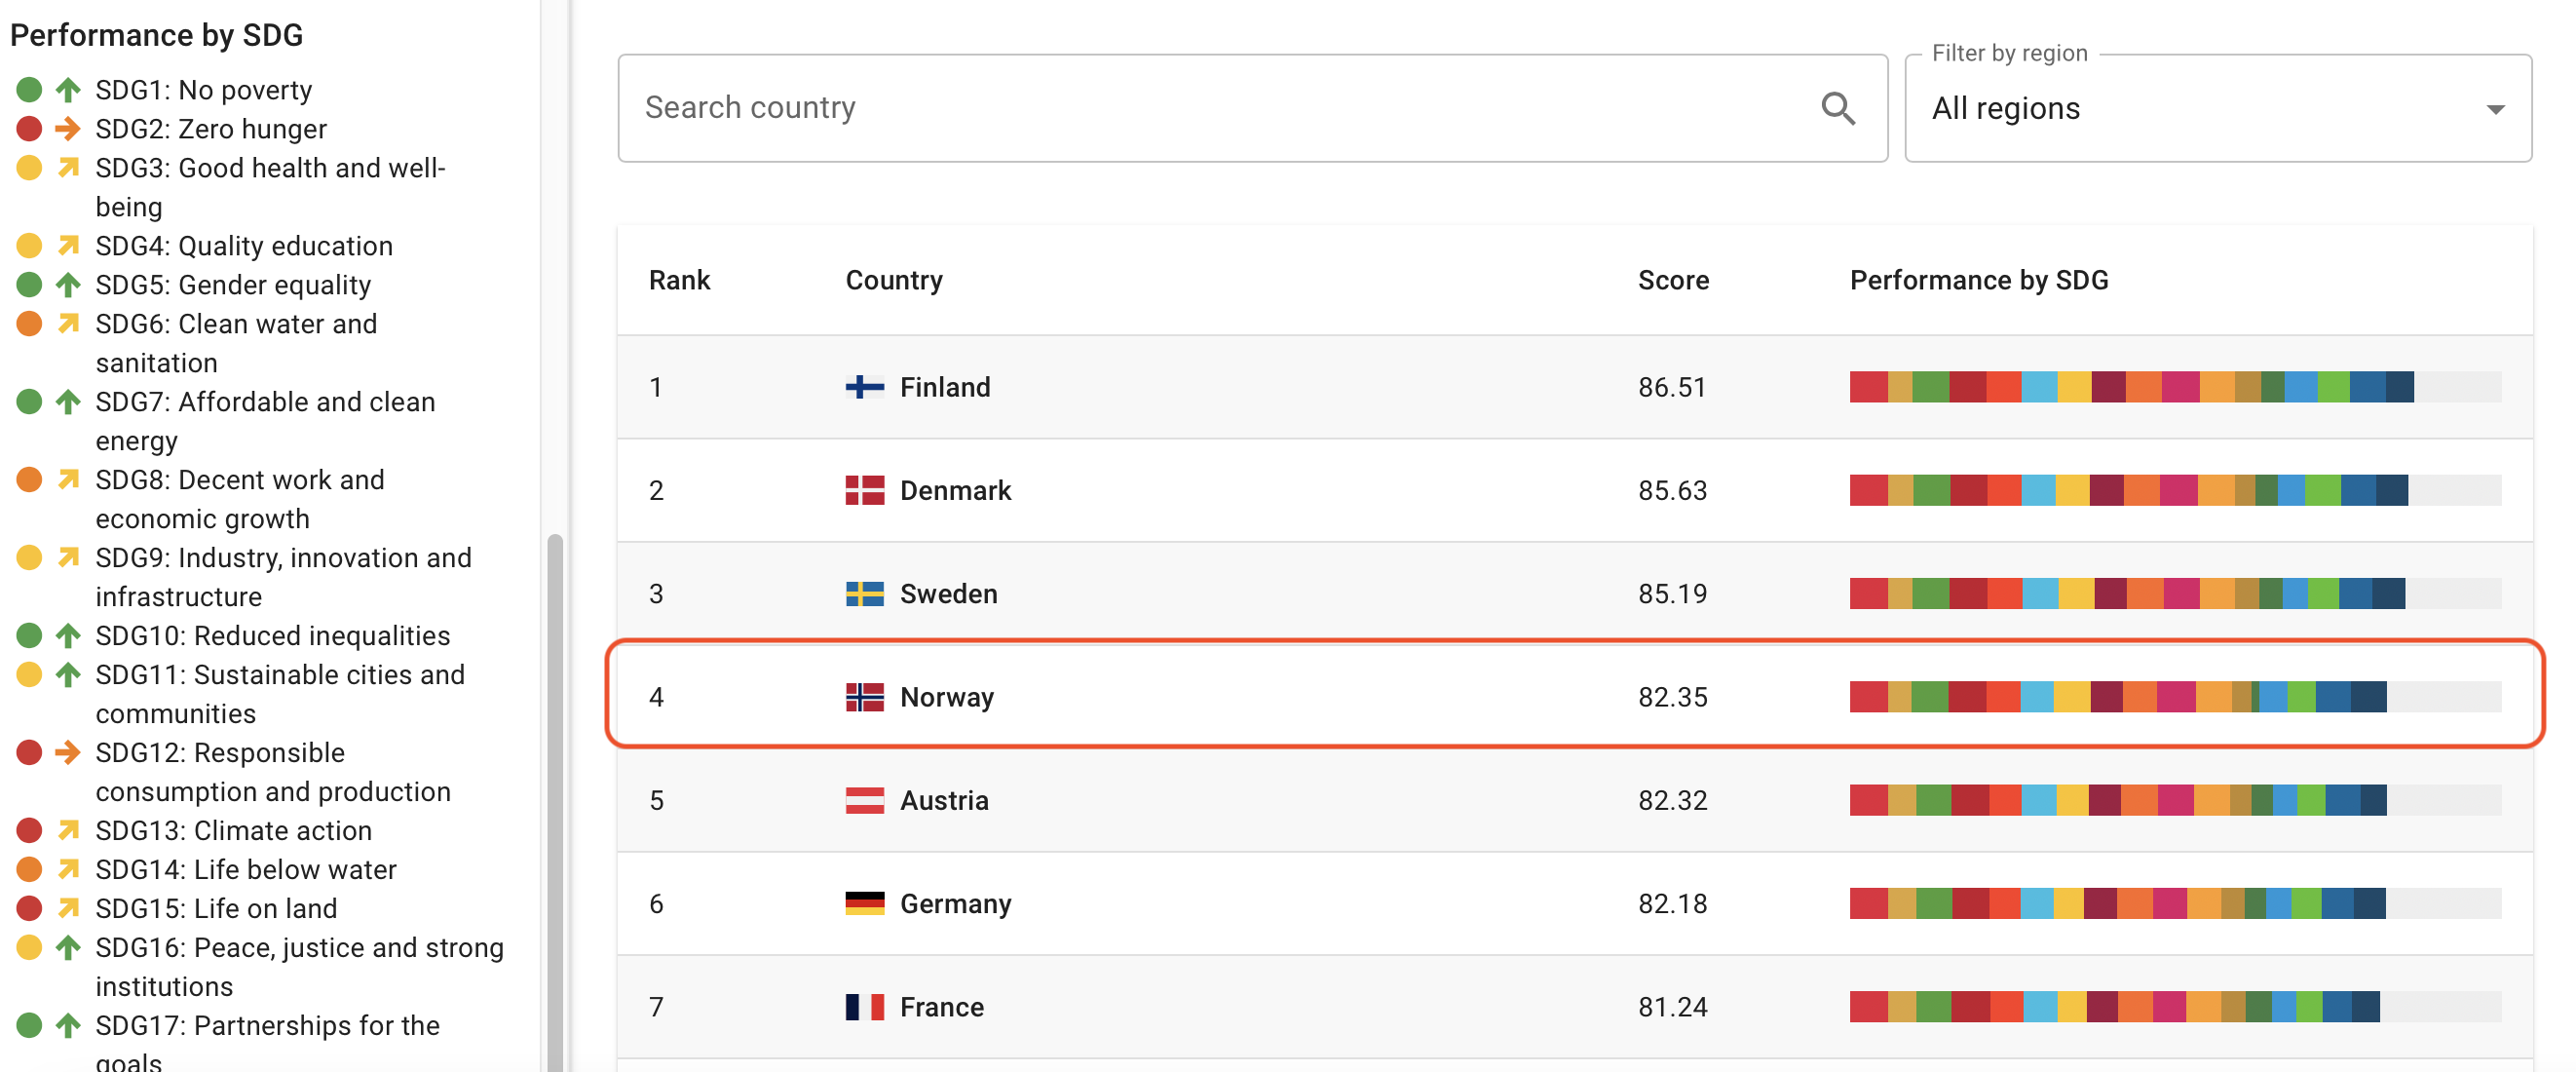
\includegraphics[scale=0.3]{Documentation/figures/sdg.png}  % largura percentual
	   \caption{SDG Index Report, source: \href{https://dashboards.sdgindex.org/rankings}{SDG Index}}
	   \label{fig:sdg}
    \end{figure}

As for Alaska:

\begin{flushright}
   \textsl{''This cash has reduced income inequality in Alaska to the lowest level in America in 2016.'' \cite{huffpost}} \\
\end{flushright}

\begin{comment}
    \vspace*{1cm}
        Dayen, D., "Alaska Gives Cash To Its Citizens Every Year. The Rest Of The U.S. Could Too", \href{https://www.huffpost.com/entry/sovereign-wealth-fund-for-america-alaska-norway_n_5b83ffb7e4b0cd327dfe878e}{HuffPost}
\end{comment}

And its Gini coefficient\footnote{"The Gini coefficient measures the extent to which the distribution of income within a country deviates from a perfectly equal distribution. A coefficient of 0 expresses perfect equality where everyone has the same income, while a coefficient of 100 expresses full inequality where only one person has all the income."- Source: \href{https://ec.europa.eu/eurostat/statistics-explained/index.php?title=Glossary:Gini_coefficient}{Europa- Statistics Explained}}:

\begin{flushright}
   \textsl{''The Gini coefficient in Alaska is 0.438 — lower than the national average and fifth lowest among all 50 states.'' \cite{247}} \\

\end{flushright}

\begin{comment}
    \vspace*{1cm}
        Stebbins, S., "How Income Inequality in Alaska Compares to Other States", \href{https://247wallst.com/state/how-income-inequality-in-alaska-compares-to-other-states/}{24/7 Wall Street}
\end{comment}

However, although that's a great start, Norway and Alaska only shares the profits of mineral wealth. And, nowadays, wealth can be generated from multiple sources.\newline


    \item \textbf{The Promise of Cryptocurrency and Blockchain Technology}


Cryptocurrencies have emerged as alternative digital currencies that operate on decentralized networks. Built on blockchain technology, cryptocurrencies offer unique features that have the potential to address some of the challenges posed by traditional financial systems. These features include transparency, immutability and accessibility. By eliminating intermediaries, cryptocurrencies provide individuals with greater control over their finances and facilitate global financial inclusion \cite{twp, cwi, coint}.

As for blockchain itself:

\begin{flushright}
   \textsl{''The idea of the sharing economy has so far come from companies like Airbnb, Uber and Lyft and has been controlled by venture capital-backed private corporations. Here’s where blockchain comes in:[...] each new robot in an autonomous vehicle fleet could be fractionally owned by every member of the community in which it operates. Every time someone purchased a ride with one of the vehicles, rather than the income only going to a private company, it could be distributed to everyone in the community.'' \cite{twp}} \\

\end{flushright}

\begin{comment}
    \vspace*{1cm}
        "Here’s how blockchain can reduce inequality", \href{https://www.washingtonpost.com/news/theworldpost/wp/2018/01/29/blockchain/}{The Washington Post}
\end{comment}

This type of reaction towards income inequality can be the brake the world needs:

\begin{flushright}
   \textsl{''Instead of waiting for the inequality to happen and then addressing it via a universal basic income, we can instead pursue the idea of a universal right to intellectual and capital goods — a universal basic capital.''} \cite{twp} \\

\end{flushright}

\begin{comment}
    \vspace*{1cm}
        "Here’s how blockchain can reduce inequality", \href{https://www.washingtonpost.com/news/theworldpost/wp/2018/01/29/blockchain/}{The Washington Post}
\end{comment}

    \item \textbf{Decentralized Finance: Empowering Financial Freedom}

    Decentralized finance builds upon the foundation of cryptocurrencies and blockchain by creating a suite of financial services and applications that are accessible to anyone with an Internet connection. Through smart contracts, decentralized lending platforms and decentralized exchanges, DeFi enables individuals to borrow, lend, trade and invest without relying on traditional financial institutions. This democratizes access to financial services and empowers individuals, particularly those in underserved communities, to participate in the global economy \cite{twp, cwi, coint}.

    \item \textbf{Tackling Global Income Inequality through DeFi}

    Can decentralized finance truly address global income inequality? While it is not a \textit{panacea}\footnote{Panacea comes from the greek \textit{Panacea}, the goddess of healing, and it's used as a term to define "the universal cure".}, DeFi has the potential to make a significant impact. By providing accessible and affordable financial services, DeFi can empower individuals in low-income communities to access capital, build businesses and improve their economic prospects. Additionally, decentralized finance reduces the barriers to entry for investment and wealth accumulation, allowing individuals to participate in previously exclusive financial markets \cite{twp, cwi, coint}.

    
\end{enumerate}


\subsection{How Dharma Network works}

Dharma Network's token, DHARM, comes as a way of tackling that inequality by, in a way, giving the worker a bonus depending on the work developed. The more and the better their work is, the more they earn.\newline

Dharma Network is accessed through a decentralized application, or DApp.\newline

Dharma Network facilitates lending and borrowing activities between users. Individuals can lend their digital assets to others and earn interest on their holdings. Borrowers, on the other hand, can access these funds by collateralizing their own digital assets. This peer-to-peer lending and borrowing model eliminates the need for intermediaries such as banks \cite{dharma}.\newline

Smart contracts (see section \ref{sc}) handle the transfer of funds, collateral management and interest payments.\newline

Borrowers on Dharma Network are required to provide collateral to secure their loans. The value of the collateral should be sufficient to cover the borrowed amount. This reduces the risk for lenders, as they have collateral to claim in case of default. Collateral is stored in smart contracts and released once the borrowed amount is repaid.\newline

Dharma Network allows lenders to set their own interest rates, creating a competitive and transparent lending environment. Borrowers can choose among available loan offers based on their preferences and the interest rates offered by lenders. The interest rates are determined by market demand and supply dynamics.\newline

Dharma Network provides a governance framework that allows users to have an equal voice in the decision-making process. This means that all users, regardless of their holding size, can participate in shaping the future of the platform. Users can vote on proposals and contribute to the development and evolution of Dharma Network \cite{dharma}.\newline

The platform is designed to be user-friendly and secure, ensuring that users can confidently engage in every activity.\newline

As for the first implementation of Dharma Network, it works as a regular cryptocurrency token, being earned manually by purchasing it. However, DHARM will soon (see chapter \ref{chap:chap4}) work as a reward token, as mentioned previously.\newline

Such concepts as Smart Contracts, Blockchain, DeFi and even Dharma Network and its token, DHARM, will be detailed in the next chapter (chapter \ref{chap:sota}) of this document.

\section{Work Plan} \label{sec:plan}

The development of Dharma Network follows a comprehensive work plan. The backend services are primarily built using Elixir, a robust and scalable programming language and the Phoenix framework. Additionally, Python is utilized for various integrations and data processing tasks. Leveraging the Algorand blockchain, Dharma Network ensures a secure and decentralized environment for users.

\section{Document Structure} \label{sec:struct}

\begin{itemize}
    \item Chapter 1- includes the objectives of the work, its context and used methodology;
	\item Chapter 2- describes the state of the art, the tools used, important concepts and related work;
	\item Chapter 3- contains a detailed description of the developed work and analysis of the requirements, such as the study objects;
	\item  Chapter 4- includes the developed work for Dharma Network, as well as other relevant information;
	\item Chapter 5- contains the analysis of the results, such as a comparison between the initial sprint planning and the execution of such sprints;
	\item Chapter 6- includes a summary of the work, a critical commentary and a discussion of future work that could be an improvement to the existing platform.
\end{itemize}


\subsection{Work Considerations}

\begin{itemize} 

	\item Backend of Dharma Network;
	\item Methodology \textbf{Scrum}\footnote{\href{https://www.atlassian.com/agile/scrum}{Scrum} is an agile project management methodology that helps teams structure and manage their work} will be used for project planning;
	\item The chosen working repository is GitHub, where the project's version control will also be done;
	\item This document is organised and described in the document structure;
	\item The organisation dossier will be on chapter \ref{sprint} and Appendix of this document.
\end{itemize} 
\newcommand{\danger}{\faIcon{exclamation-triangle}}

\chapter{State of the Art} \label{chap:sota}

%\usepackage{caption}

 In this initial phase of the project, the deliverable pieces are as follows:

 \begin{itemize}
     \item Background, consisting of:
     \begin{itemize}
         \item Frameworks
        \item IDE
        \item Others
    \end{itemize}
     \item Existing Solutions
 \end{itemize}


\section{Background}

Dharma Network's technical foundation is built upon the Algorand blockchain, a \textit{leading blockchain platform} known for its scalability, security and efficiency. The utilization of \textit{Elixir}, \textit{Phoenix} and \textit{Python }technologies enables the development of robust and performant backend services, ensuring seamless interactions between the Dharma Network frontend and the blockchain infrastructure.

As it is an extensive project, Dharma Network compiles an extraordinary variety of languages and frameworks.
For the frontend, it uses \textit{Typescript} and \textit{VueJS}, although this report will focus on the backend and blockchain section. \newline

\subsection{Backend technologies and frameworks}

In the world of software development, the backend plays a crucial role in powering applications and enabling seamless communication between the user interface and the underlying data and systems.\newline

The backend services are mostly written in Elixir, with some functionalities implemented in TEAL, Tealish and Python, with the help of PyTEAL.

\subsubsection{Elixir}\label{elixir}

\textit{Elixir}\footnote{\href{https://elixir-lang.org}{Elixir} is a fault-tolerant, low-latency, dynamic language that is used for building scalable and maintainable applications, such as Discord and Heroku} is a functional programming language based on \href{https://www.erlang.org}{Erlang}\footnote{For a further understanding on Erlang, please check: https://www.erlang.org} \cite{elixir}. \newline

A \textit{functional programming language} consists of developing software with pure functions to create maintainable code. Every function needs to return something and those functions can be used as anything, from variables to arguments. It creates clean and elegant code with immutable data, unlike imperative programming, which doesn't have immutability as a core principle. Functional programming focuses on what needs to be done by defining the relationships and transformations of data. For this matter, errors can quickly be identified and corrected \cite{func}.\newline

Some \textit{key principles of functional programming} are:

\begin{enumerate}
    \item \textit{Pure Functions:} In functional programming, functions are pure, meaning they do not have any side effects and always produce the same output given the same input. Pure functions avoid shared state and mutable data, resulting in more predictable and testable code.
    \item \textit{Immutability:} Data in functional programming is immutable, meaning it cannot be modified once created. Instead of updating values in place, new data structures are created, facilitating a more controlled and predictable system state.
    \item \textit{Higher-Order Functions:} Functional programming encourages the use of higher-order functions, which treat functions as first-class citizens. This allows functions to be passed as arguments, returned as values and composed together, leading to more modular and reusable code.
    \item \textit{Recursion:} Instead of using loops for iteration, functional programming favors recursion. Recursion allows functions to call themselves, enabling elegant and concise solutions to complex problems \cite{func}.
\end{enumerate}

With this being said, some \textit{benefits of functional programming} are:

\begin{itemize}
    \item \textit{Modularity and Reusability:} By promoting the use of pure functions and immutability, functional programming enables developers to create small, composable functions that can be reused in different contexts. This modularity leads to code that is easier to maintain and extend.
    \item \textit{Concurrency and Parallelism:} Functional programming encourages the use of immutable data, which eliminates the need for locks and synchronization. This makes it easier to reason about concurrent and parallel execution, allowing for efficient utilization of modern hardware.
    \item \textit{Error Handling:} With its emphasis on immutability and pure functions, functional programming provides a natural way to handle errors. By separating the pure computation from the error handling logic, developers can write more robust and predictable error handling code \cite{func}.
\end{itemize}

\textbf{Modules in Elixir}\newline

In Elixir, code is organized into modules. A module is a collection of functions, data types and state. It serves as a unit of code organization and encapsulation, enabling developers to group related functionality together. Modules are defined using the \texttt{defmodule} keyword followed by the module name.

Within a module, functions are defined using the \texttt{def} keyword. These functions can be public or private, where public functions are accessible from other modules, and private functions are intended for internal use within the module. Elixir follows the convention of naming files after their corresponding module, allowing for easy navigation.

Modules also support the concept of behaviors, which define a set of functions that a module must implement. Behaviors enable the creation of generic code that can be reused by multiple modules.\newline

\textbf{Mix: Build Tool and Dependency Manager}\newline

\textit{Mix} is a central component of the Elixir ecosystem. It serves as a build tool, task runner and dependency manager for Elixir projects. \textit{Mix} provides a range of tasks, such as compiling code, running tests, managing dependencies and generating documentation. It automates common development tasks and makes it easy to manage the project's lifecycle.

One of the key features of Mix is its dependency management system. With a simple configuration file \texttt{(mix.exs)}, developers can specify the required dependencies for their project. Mix fetches, compiles and manages these dependencies, ensuring that the project's dependencies are correctly resolved and up to date.

Mix also supports the creation of new projects from predefined project templates, allowing developers to quickly bootstrap their applications with a predefined structure and initial configuration.\newline


\subsubsection{Phoenix Framework}

\textit{Phoenix}\footnote{\href{https://www.phoenixframework.org}{Phoenix framework} supports all kinds of resources and languages, such as HTML5, Elixir, database connections, JSON encoding and decoding, etc} is a web development framework written in Elixir and it implements an \textit{MVC} pattern, denominated Model-View-Controller, which means it's divided into 3 layers: \textit{view}, responsible for the interaction with the user; \textit{model}, responsible for the access and manipulation of the data; \textit{controller}, responsible for connecting model and view \cite{phoenix}.\newline

Phoenix works by plugs, its basic element. They come from the Plug library and transform the \texttt{Conn} data structure. This \texttt{Conn} contains every information about the request and response in HTTP connections.\newline

Phoenix's workflow (see figure \ref{fig:phx_work}) can be described as follows:

\begin{enumerate}
    \item Receives a request
    \item Converts request to \texttt{Conn}
    \item \texttt{Conn} passes through several plugs
    \item It renders a response.
\end{enumerate}

\begin{figure}[htbp]
	\centering
	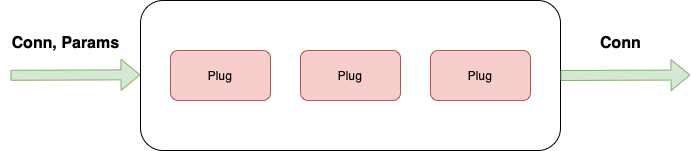
\includegraphics[scale=0.4]{Documentation/figures/phx_work-3.png}  % largura percentual
	\caption{How Phoenix Works, source: \href{https://blog.logrocket.com/build-rest-api-elixir-phoenix/}{LogRocket}}
	\label{fig:phx_work}
\end{figure}

Let's take a closer look to Phoenix's lifecycle (see figure \ref{fig:phx_lc}):\newline

\begin{figure}[htbp]
	\centering
	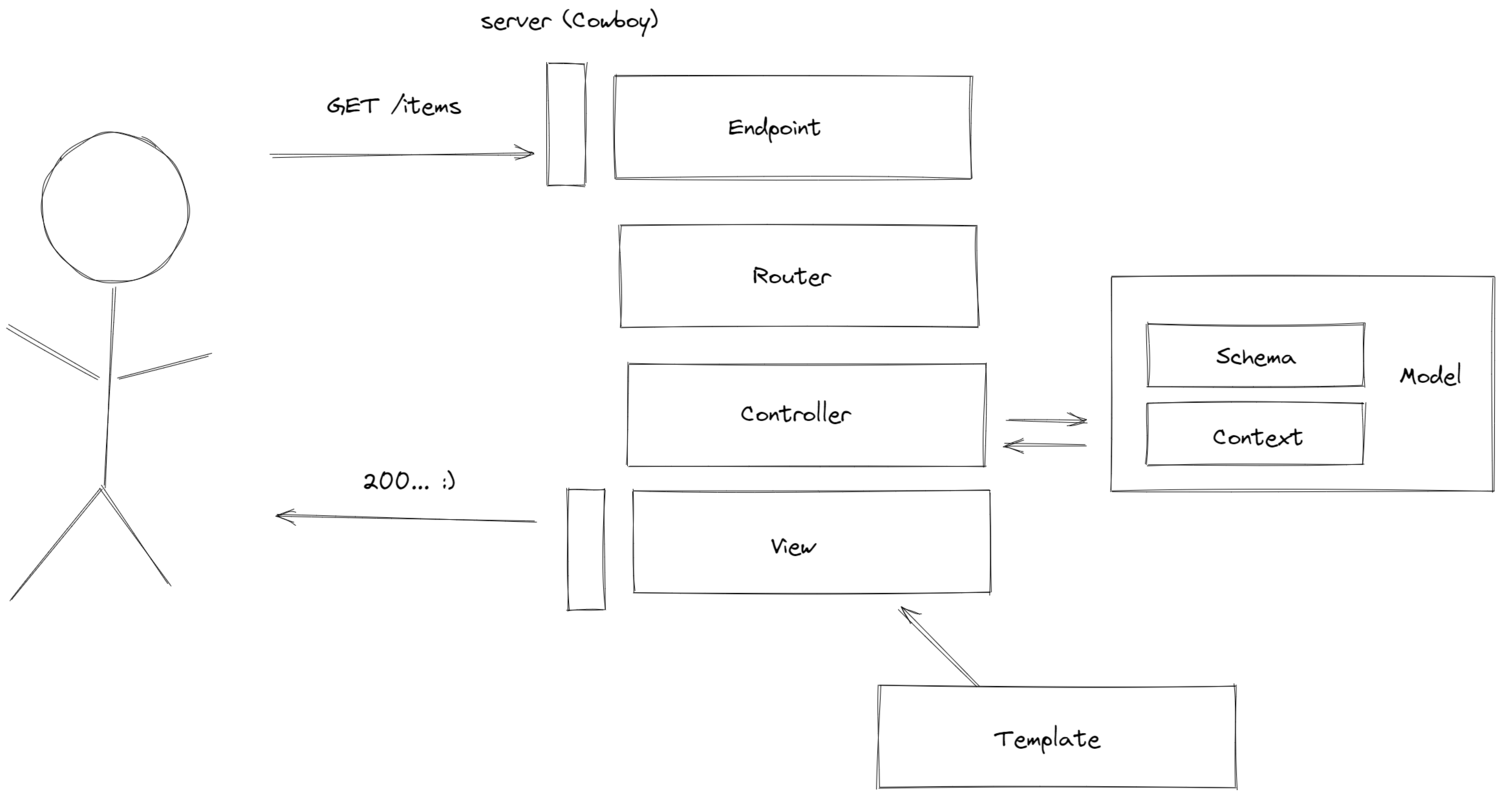
\includegraphics[scale=0.2]{Documentation/figures/phx_lifecycle.png}  % largura percentual
	\caption{Phoenix's Lifecycle, source: \href{https://serokell.io/blog/introduction-to-phoenix}{Serokell}}
	\label{fig:phx_lc}
\end{figure}

"Phoenix receives a request at the endpoint and the endpoint converts it into a \texttt{Conn} data structure, forwarding it to the router.\newline

The router pipelines the \texttt{Conn} data structure into the controller and the controller interacts with the model to fetch data from the database and render it using templates. Templates can be HTML or JSON files. Here, the endpoint, router and controllers are plugs — everything in Phoenix is a composable function that transforms data into different structure." \cite{phx}\newline


Some advantages of Elixir and Phoenix are:

\begin{itemize}
    \item \textit{Fault-Tolerance and Scalability:} Built on the battle-tested BEAM VM, Elixir and Phoenix provide fault-tolerant capabilities, enabling systems to handle failures gracefully and continue running uninterrupted. Additionally, Elixir's lightweight concurrency model allows for efficient utilization of system resources, making it highly scalable.
    \item \textit{Real-Time and Concurrent Capabilities:} Elixir and Phoenix excel in building real-time applications that require concurrent processing, such as chat systems, collaborative tools and IoT applications. With the built-in support for channels and distributed systems, Phoenix enables developers to create responsive and interactive user experiences.
    \item \textit{Speed:} Elixir and Phoenix are extremely fast, since they compile into BEAM bytecodes and have the speed benefits of Erlang without having the performance issues \cite{adv}.

\end{itemize}


\subsubsection{TEAL}

\href{https://developer.algorand.org/docs/get-details/dapps/avm/teal/}{\textit{TEAL}}, short for "Transaction Execution Approval Language", is the native smart contract language of the Algorand blockchain. It is specifically designed to provide a simple and efficient way to write secure and scalable smart contracts. TEAL is a low-level, stack-based language that operates on Algorand's transactional model. It consists of thirty basic functions.\newline

The main objective of TEAL is to enable developers to express complex logic and conditions that govern the execution of transactions. It allows for the creation of smart contracts that can perform various operations, such as transferring assets, validating conditions and executing custom logic. TEAL contracts are embedded within Algorand transactions, ensuring their atomicity and immutability \cite{teal, teal_2}.\newline

TEAL supports both Stateful and Stateless Smart Contracts (see section \ref{sc}) and those can also be written in Python and compiled by PyTEAL library to TEAL (see section \ref{python} for a further understanding).\newline

To a better understanding of TEAL's workflow, please read section \ref{algo_bc} and see figures \ref{fig:algo} and \ref{fig:algoflow}.

\subsubsection{Tealish}

\href{https://github.com/tinymanorg/tealish}{\textit{Tealish}}, on the other hand, is a higher-level framework introduced by \href{https://tinyman.org}{Tinyman.org}, designed to enhance the development experience of smart contracts on the Algorand blockchain. It provides additional features and abstractions that simplify contract development and improve code readability.\newline

Tealish introduces a more declarative and expressive syntax that abstracts away some of the low-level complexities of TEAL. It allows developers to write smart contracts using a familiar programming style, resembling traditional programming languages. This higher-level abstraction makes contract development more accessible to a broader range of developers.\newline

Furthermore, Tealish focuses on code reusability and composability, allowing developers to create modular contract components that can be easily combined and integrated into larger systems. This modularity enhances code maintainability and fosters the development of scalable and extensible smart contract applications \cite{tealish}.\newline

Some of the \textit{key features and concepts} offered by Tealish include:

\begin{itemize}
    \item \textit{Python-like syntax:} Tealish is designed to resemble the Python programming language, making it familiar and accessible to developers who are already comfortable with Python.
    \item \textit{High-level constructs:} Tealish introduces high-level constructs that abstract away some of the complexities of TEAL, allowing developers to focus on the logic of their smart contracts. These constructs include conditional statements, loops, function definitions and more.
    \item \textit{Static analysis:} Tealish includes a static analyzer that performs checks and provides feedback on potential issues or errors in the code. This helps catch mistakes early in the development process and improves code quality.
    \item \textit{PyTEAL integration:} Tealish seamlessly integrates with PyTEAL, a Python library for compiling TEAL code. This integration allows developers to write their smart contracts using Tealish and then compile them into TEAL using PyTEAL.
\end{itemize}

By providing a higher-level language for writing smart contracts, Tealish aims to simplify the development process and reduce the learning curve associated with TEAL. It can be particularly useful for developers who are more comfortable with Python or prefer a more expressive syntax when working with smart contracts on the Algorand blockchain \cite{tealish}.

\subsubsection{Python}\label{python}

Python is one of the languages that has experienced most growth over the last few years, due to its simplicity and versatility. It also provides a vast library with plentiful resources ready to be implemented, as well as multi platform performance, since the same code can easily be executed on every operative system, whether it's Linux, MacOS or Windows, without the need to be changed.\newline

When it comes to Smart Contracts, in Algorand, they can be written in Python, through the help of \textit{PyTEAL}.\newline

\href{https://github.com/algorand/pyteal}{PyTEAL} allows developers to express complex logic and conditions in a familiar programming language like Python, and then compile it into TEAL.\newline

PyTEAL is a Python library that provides an abstraction layer for writing smart contracts in Algorand. It allows developers to leverage the expressive power of Python to define the logic and conditions of their smart contracts.\newline

Developers can write smart contracts in Python using PyTEAL by defining the desired logic and conditions. They can use Python's control flow statements, variables, functions and libraries to implement the desired behavior of the smart contract.
PyTEAL provides specific constructs and functions to interact with the Algorand blockchain, such as creating transactions, validating conditions and transferring assets.\newline

Once the Smart Contract is ready, it needs to be compiled into TEAL. For that, PyTEAL provides a compilation step that converts the Python code into TEAL bytecode.
The compiled TEAL bytecode can be embedded in Algorand transactions and deployed on the blockchain \cite{pyteal}.\newline

While PyTEAL and Tealish serve similar purposes, there are some \textit{differences} between the two:

\begin{itemize}
    \item \textit{Syntax:} PyTEAL is a \textit{Python library} that allows you to write TEAL code using Python syntax. It provides a way of constructing TEAL programs by using Python functions and constructs. On the other hand, Tealish is a \textit{separate programming language} that resembles Python but is specifically designed for writing Algorand smart contracts. Tealish introduces its own syntax and constructs, which are higher-level than TEAL but still compile down to TEAL code.
    \item \textit{Integration:} PyTEAL integrates directly with the Python ecosystem. It allows you to write TEAL code as Python functions and seamlessly integrate them into your Python-based Algorand applications. PyTEAL provides a convenient way to generate TEAL code using the power and flexibility of Python. On the other hand, Tealish is a standalone language that needs to be separately installed and used alongside PyTEAL. Tealish is used to write the logic of the smart contracts in a more expressive and abstract manner, and then the Tealish code is compiled into TEAL using PyTEAL.
    \item \textit{Abstractions:} Tealish offers higher-level constructs and abstractions that simplify the process of writing smart contracts. It provides a more expressive syntax similar to Python, allowing developers to focus on the logic of their contracts without getting lost in the intricacies of TEAL. PyTEAL, on the other hand, primarily focuses on providing a Python interface for generating TEAL code, but it does not introduce additional abstractions beyond what TEAL itself offers.
\end{itemize}


\subsubsection{Visual Studio Code}

\href{https://code.visualstudio.com}{Visual Studio Code} (VS Code) is a widely popular source code editor developed by Microsoft. It is known for its versatility, extensive plugin ecosystem and cross-platform support. With features like intelligent code completion, debugging support, and Git integration, VS Code enhances developers' productivity and efficiency. Its lightweight nature and customizable interface make it a preferred choice for developers across different programming languages.\newline

All the code was developed on Visual Studio Code.

\subsubsection{PostgreSQL and PG-Admin} \label{post}

\href{https://www.postgresql.org}{\textit{PostgreSQL}} is a powerful open-source relational database management system (RDBMS). It offers robust data integrity, high performance and advanced features, making it a popular choice among developers and enterprises. With support for complex queries, transactions and advanced indexing options, PostgreSQL enables the development of scalable and reliable database-driven applications. Its community-driven development and regular updates ensure its continued growth and relevance in the industry.\newline

The tool used to interact with the database is  \textit{PG-Admin}. PG-Admin is an open-source administration and development platform specifically designed for PostgreSQL. It provides a user-friendly graphical interface that allows users to easily perform various tasks such as creating and managing databases, executing SQL queries, monitoring database performance and much more.\newline

Every database used/created during the internship was PostgreSQL and the main tool used to control it was PG-Admin.\newline


\subsubsection{ITerm 2}

\href{https://iterm2.com}{\textit{ITerm 2}} is an advanced terminal emulator for MacOS. It provides a feature-rich command-line interface, enhancing developers' experience and productivity. \textit{ITerm 2} offers a wide range of functionalities such as split panes, hotkey navigation, session management and extensive customization options. Its support for profiles, triggers and scripting capabilities make it a versatile tool for developers working with command-line interfaces.\newline

\textit{ITerm 2} was used during the project to run and test the code.

\subsubsection{Jira- Atlassian}

\textit{Jira} is a popular project management and issue tracking tool developed by Atlassian. It provides teams with a centralized platform to plan, track and manage software development projects efficiently. With features like task tracking, agile boards, workflow customization and collaboration capabilities, Jira enables teams to streamline their development processes and improve overall project visibility. It integrates seamlessly with other Atlassian tools like Confluence and Bitbucket, creating a comprehensive ecosystem for software development teams.\newline

\textit{Jira} was used during the internship to keep track of the tasks and create new tickets.

\subsection{Blockchain} \label{blockchain}

Blockchain was firstly introduced to the world in 1991, as a way of storing and securing digital data. It consists of a distributed database, otherwise known as ledger, shared among a computer network's nodes. Several parties can access it at once and that particular feature is part of its primary benefit- data can't be altered. In order for a block to be modified, all parties need to be involved, which is a complex procedure, making each block, specifically its data, immutable.\newline

Blockchain works as a peer-to-peer system, making third parties obsolete, such as auditors or other humans that can cause errors and charge fees. Its encryption feature makes it always secure, transactions are done instantly and transparently, since the ledger is automatically updated and the transactions' authenticity is verified and confirmed by its members. \newline

Each new record creates a new block with a unique and identifying hash\footnote{A hash function is a mathematical function that converts a given input value into a shorter, fixed-length value, that represents the original string of characters.}. Blocks are then linked into a chain of records, forming a blockchain \cite{bc}. \newline

For a better understanding of this subject, let's get a closer look of \textit{fundamental components of a blockchain}: \newline

A \textbf{transaction} represents the fundamental units of data exchange within a blockchain network. Each transaction encapsulates essential information, such as sender, recipient and the amount being transferred.

They are cryptographically signed to ensure their authenticity and integrity.\newline

\textbf{Transaction Validation:}\newline

Before a transaction can be included in a block, it undergoes a validation process.
The validation process verifies the transaction's legitimacy, ensuring that the sender has sufficient funds and adheres to predefined rules and protocols.
Validation is performed by network nodes, which collectively maintain the blockchain's consensus mechanism.\newline

\textbf{Transaction Propagation:}\newline

Once validated, the transaction propagates across the network, reaching all participating nodes.
Nodes receive and verify the transaction independently, maintaining a distributed ledger that reflects the transaction's history.\newline


\begin{figure}[htbp]
	\centering
	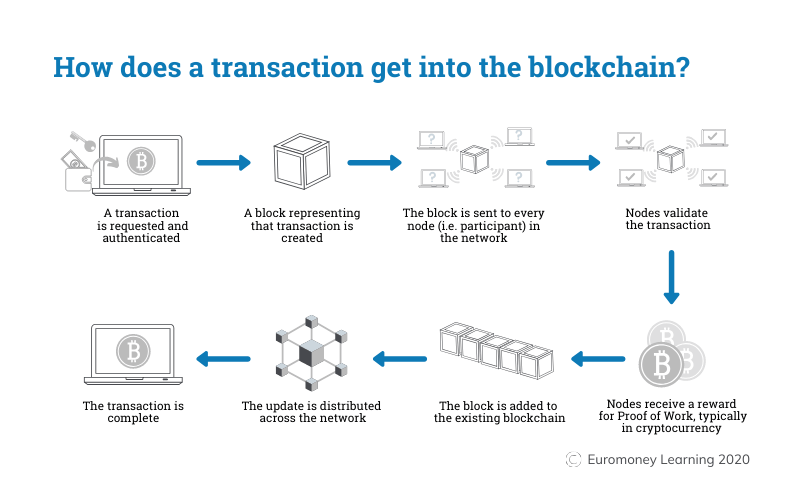
\includegraphics[scale=0.5]{Documentation/figures/transact.png}  % largura percentual
	\caption{How does a transaction get into the blockchain, source: \href{https://www.euromoney.com/learning/blockchain-explained/how-transactions-get-into-the-blockchain}{EuroMoney}}
	\label{fig:trans}
\end{figure}

A \textbf{block} is a collection of transactions bundled together.
Each block contains a unique hash, a timestamp and a reference to the previous block.
The previous block reference creates a chain-like structure \footnote{Chains are a linked list of blocks. They are immutable and append-only. A blockchain architecture may have one or more chains. Chains can grow to an infinite length or number of blocks. This can be prevented or managed by pruning, but pruning has side effects that reduce the trust in the blockchain network and remove the ability to explore and audit the entire chain. This can reduce the integrity of the chain- \href{https://www.oreilly.com/library/view/hands-on-smart-contract/9781492086116/ch01.html}{O'Reilly}.}, forming the blockchain.\newline


\textbf{Block Formation:}\newline

Miners, specialized participants in the network, compete to add the next block to the chain.
Miners group validated transactions into candidate blocks.\newline
To secure the blockchain, miners must solve a complex mathematical puzzle, known as proof of work, which requires substantial computational power.
The first miner to solve the puzzle broadcasts their solution to the network, earning the right to add their block to the chain.\newline

\textbf{Block Verification and Consensus:}\newline

Upon receiving a new block, network nodes independently verify its validity.
Nodes ensure that the transactions within the block adhere to the predefined rules and protocols.
Consensus mechanisms, such as Proof of Work or Proof of Stake, ensure agreement among nodes regarding the validity of the block.
Block Confirmation and Chain Extension:
Once a block is verified and accepted by the network, it becomes a permanent part of the blockchain.
The block's hash is used as a reference in subsequent blocks, creating an immutable and tamper-resistant record of transactions.
New blocks are added to the chain, extending its length and reinforcing the security of the entire blockchain network.\newline

In the following image (\ref{fig:blocks}), it's proposed an example of how the interaction (the evolution of a transaction) between blocks work:\newline

\begin{figure}[htbp]
	\centering
	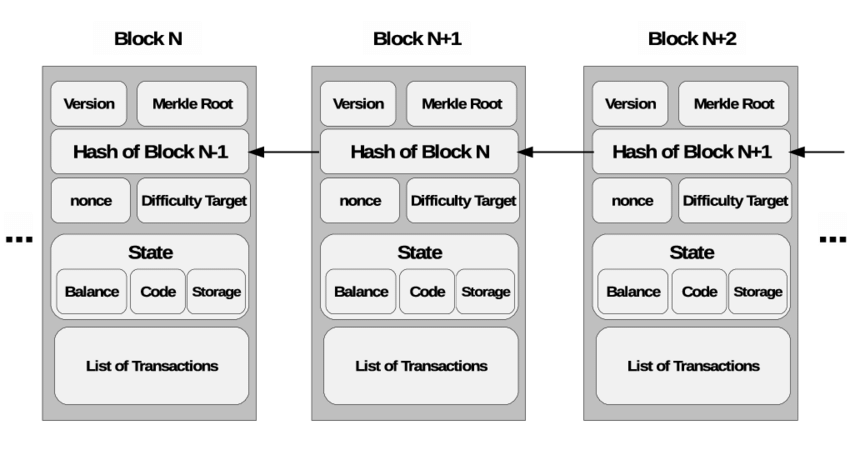
\includegraphics[scale=0.5]{Documentation/figures/blockchain.png}  % largura percentual
	\caption{Chained blocks creating a blockchain, source: \href{https://www.researchgate.net/figure/Blockchain-design-structure-showing-chained-blocks-with-header-and-body-fields_fig2_321017113}{Research Gate}}
	\label{fig:blocks}
\end{figure}

A \textbf{node} on a blockchain means an electronic device that guards an IP address and it's responsible for running the blockchain's algorithm to verify and authenticate each transaction. They contain a copy of blockchain's primary protocol and its entire transaction history \cite{node}.\newline

Nodes can have 3 various roles when being part of a blockchain \cite{node_type}:

\begin{itemize}
    \item \textbf{Maintaining the blockchain:}
    
Nodes store the data of the blockchain (as mentioned, its primary protocol and transaction history) and help keeping it scalable. 
    
    \item \textbf{Validating a transaction:}

    Some nodes are part of consensus algorithms (see \ref{cons.mec}), while others just store transaction records. The process involves receiving a transaction order, verifying its authenticity and deciding whether or not to accept it, and recording it on the ledger.
    
    \item \textbf{Accessing information:}

    To access any type of information on the ledger, an interaction with nodes needs to be made. 
\end{itemize}

There are 10 major node types, divided into 4 categories \cite{node_type}:

\begin{enumerate}
    \item \textbf{Full Node:}

    Most ocurrent node. These are responsible for storing the records os the transactions on the ledger. Also defined as the \textbf{servers} of the blockchain. They participate in consensus mechanisms and contribute to the governance of the blockchain. Two types of full nodes are:

    \begin{itemize}
            \item \textbf{Pruned Full Node:}

     These nodes store data on the hard disk by pruning older blocks. They retain a defined amount of recent transaction records, removing the need to store the entire blockchain history. Pruned full nodes strike a balance between storage efficiency and network participation.\newline
    
    \item \textbf{Archival Full Node:}

    As the name suggests, archival full nodes store and maintain the entire blockchain database without any storage limitations. These nodes play a critical role in ensuring the long-term integrity of the blockchain by preserving a comprehensive record of all transactions.
    
Within the category of archival full nodes, there are various specialized nodes:\newline

\begin{itemize}
    \item \textbf{Authority Node:}

    In certain private or partially-centralized blockchains, only a select group of authority nodes have permission to access and manage the blockchain. These nodes exercise control and restrict access to the network.\newline
    
    \item \textbf{Miner Node:}

    Commonly found in Proof of Work-based blockchains like Bitcoin, miner nodes solve complex mathematical problems to validate and add new blocks of transactions to the blockchain. In return for their computational efforts, miners are rewarded with newly minted tokens.\newline
    \item \textbf{Staking Node:}

    These nodes are integral to blockchains utilizing the Proof of Stake consensus model. To participate as a staking node, users must lock a certain amount of native tokens in the network. The blockchain system randomly selects staking nodes to process transactions and record them on the ledger based on predefined rules, such as token holdings or duration of participation.\newline
    \item \textbf{Masternode:}

    Masternodes perform additional functions beyond validating and recording transactions. They serve specific purposes defined by the blockchain network, such as facilitating advanced governance mechanisms or providing specialized services. Dash, an early adopter of masternodes, implemented this concept in its network mechanism.\newline
    
\end{itemize}
    \end{itemize}
    
    \item \textbf{Light Node:}

    Also known as Simplified Payment Verification (SPV) nodes, light nodes store only necessary information such as block headers instead of the entire blockchain. They offer faster transactions and require less storage.

    Designed for efficiency and convenience, light nodes prioritize faster transactions and day-to-day activities. Unlike full nodes, which store the entire blockchain, light nodes store only the necessary information, typically block headers. This streamlined approach reduces storage requirements and allows for quicker synchronization with the blockchain network.\newline
    
    \item \textbf{Lightning Node:}

    These nodes reduce transaction latency by enabling off-chain transactions, minimizing the load on the network and facilitating instantaneous and low-cost transactions.

    When blockchain networks experience high traffic and congestion, lightning nodes come into play. These nodes enable off-chain transactions by establishing direct connections between users, bypassing the need for every transaction to be recorded on the main blockchain. Lightning nodes significantly reduce transaction latency and minimize fees, making microtransactions more viable.\newline
    
    \item \textbf{Super Node:}

    Super nodes perform specialized tasks within a blockchain network, such as maintaining network regulations or implementing upgrades.

    Although less common, super nodes have distinct roles tailored to specific blockchain networks. They may be responsible for maintaining network regulations, implementing protocol upgrades, or supporting specialized functionalities within the blockchain ecosystem.\newline
\end{enumerate}

Understanding the diverse types of blockchain nodes is essential for developers, businesses, and users alike. Developers leverage this knowledge to create efficient decentralized applications, while businesses can optimize their operations and build cost-effective solutions. Users benefit by gaining insights into the underlying infrastructure and making informed decisions based on their specific requirements.\newline

Blockchain nodes are the foundational building blocks of decentralized networks. Their roles collectively contribute to the robustness and reliability of blockchain technology.\newline


A \textbf{fork} occurs when a community proposes changes to the blockchain's protocol or underlying rules, either for efficiency or concerning matters. These changes result in the separation of the blockchain, giving rise to a new blockchain that shares the entire transaction history but embarks on a different path. This way, forks enable DeFi to enhance security, introduce new functionalities, address security risks or create an entire new coin and ecosystem \cite{fork}.


\begin{figure}[htbp]
	\centering
	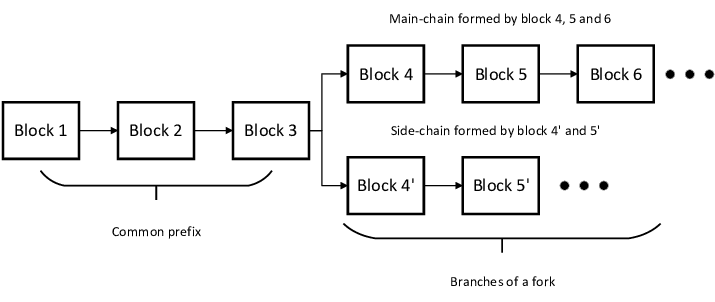
\includegraphics[scale=0.4]{Documentation/figures/fork.png}  % largura percentual
	\caption{Fork structure, source: \href{https://www.researchgate.net/figure/Fork-structure-in-a-blockchain_fig2_342017074}{Research Gate}}
	\label{fig:fork}
\end{figure}

Forks can be if two main types: soft forks and hard forks \cite{fork}.

\begin{itemize}
    \item \textbf{Soft Forks:}

    Soft forks are analogous to software updates for the blockchain.
When universally adopted by users, soft forks establish new rules for a cryptocurrency.
These are typically employed to introduce new programming functions or features.
As soft forks maintain a single blockchain, the changes are backward compatible with pre-fork blocks. As an example, there's SegWit's upgrade, Bitcoin's Segregated Witness protocol.\newline
    \item \textbf{Hard Forks:}

    A hard fork occurs when the code undergoes significant changes, rendering the new version incompatible with older blocks.
In this scenario, the blockchain splits into two: the original blockchain and a new version adhering to new rules.
Hard forks give rise to entirely new cryptocurrencies, spawning well-known coins such as Bitcoin Cash and Bitcoin Gold, derived from the original Bitcoin blockchain.

\end{itemize}

\begin{figure}[htbp]
	\centering
	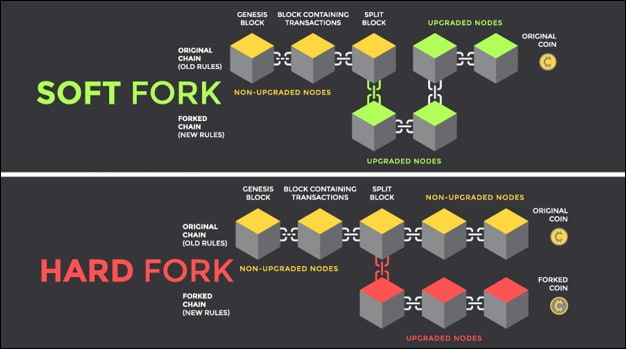
\includegraphics[scale=0.5]{Documentation/figures/fork_type.jpeg}  % largura percentual
	\caption{Fork types, source: \href{https://shardeum.org/blog/what-is-a-blockchain-fork/}{Shardeum}}
	\label{fig:fork_type}
\end{figure}



\subsubsection{Consensus Mechanism} \label{cons.mec}

To ensure maximum security in each node, there are some mechanisms to approve the addition of a new node to the chain. They are also used to keep the ledger updated in every node. \par
Since blockchain doesn't require third parties, no authority can declare that a certain version of the data is correct and verified, which brings up the question: \textit{how is that veracity proved?} \newline
That's where consensus mechanisms come in. Some of the most popular are \textit{Proof-of-Work (PoW}, \textit{Proof-of-Stake (PoS)} and \textit{Practical Byzantine Fault Tolerant Mechanism}:\newline

\begin{itemize}
    \item \textbf{Proof-of-Work (PoW)}:
    
    PoW is the consensus mechanism used by Bitcoin and many other cryptocurrencies. In PoW, nodes in the network compete to solve complex mathematical puzzles, requiring significant computational power. The first node to solve the puzzle earns the right to add the next block to the blockchain, which means newly minted cryptocurrency.\newline
    This process is resource-intensive and time-consuming, making it difficult for an attacker to tamper with the blockchain. The proof of solving the puzzle is then shared with the network, allowing other nodes to verify and reach consensus on the validity of the new block. The nodes responsible for the problem solving are called miners and its process is called mining. Miners can be rewarded with a certain amount of the cryptocurrency if they contribute to the solution \cite{hack}.

    \item \textbf{Proof-of-Stake (PoS)}: 
    
    PoS is an alternative consensus mechanism that aims to address the resource consumption of PoW. In PoS, the creator of the next block is chosen in a deterministic way, based on their stake or ownership of the cryptocurrency. Instead of solving puzzles, validators, also known as stakeholders, are selected to validate transactions and create new blocks based on their existing stake. Validators are incentivized to act honestly, as their stake can be penalized if they behave maliciously. PoS is considered to be more energy-efficient compared to PoW and allows for faster block generation times \cite{hack}.

    \item \textbf{Practical Byzantine Fault Tolerant (PBFT) Mechanism}: 
    
    PBFT is a consensus mechanism designed for distributed systems, including blockchain networks. It focuses on reaching consensus among a set of nodes even if some of them are faulty or malicious (Byzantine faults). PBFT ensures that the majority of nodes agree on the order of transactions, and once a block is approved by the network, it is considered final. This mechanism is often used in permissioned blockchain networks where the participants are known and trusted \cite{hack}.

\end{itemize}

\subsubsection{Smart Contracts}\label{sc}

Smart contracts are an important and complex part of a blockchain.

These are defined as computer programs stored on a blockchain that automatically execute (when predetermined needs are met) and enforce contractual agreements without the need for intermediaries.

Its structure follow a simple \textit{"if/when...then" logic}, where participants agree upon specific conditions and corresponding actions.
Once the conditions are met and verified by a network of computers, the smart contract automatically executes the specified actions. Let's see an example:\newline

"\textit{(...) \textbf{IF} you send object A, \textbf{THEN} the sum (of money, in cryptocurrency) will be transferred to you.
\textbf{IF} you transfer a certain amount of digital assets (cryptocurrency, for example, ether, bitcoin), \textbf{THEN} the A object will be transferred to you.
\textbf{IF} I finish the work, \textbf{THEN} the digital assets mentioned in the contract will be transferred to me (...)}" \cite{sc}.\newline

Some of its key benefits and features are:

\begin{itemize}
    \item \textit{Autonomy:} Smart contracts operate autonomously, eliminating the need for manual or third parties intervention.
    \item \textit{Self-Enforcement:} They automatically execute contract terms and enforce obligations.
    \item \textit{Immutable:} Contract terms and conditions cannot be altered once deployed on the blockchain.
    \item \textit{Trustless:} Smart contracts rely on cryptographic protocols and decentralized consensus, reducing the need to trust intermediaries.
    \item \textit{Distributed:} They are replicated and distributed across all nodes connected to the network, ensuring all participants have a copy of its conditions.
    \item \textit{Deterministic:} Smart contracts operate based on predefined functions that are executed only when specific conditions are met, so its outcome will remain consistent, regardless of who executes the contract, ensuring predictable and reliable results.
    \item \textit{Customizable:} They offer flexibility for customization and modification before being launched. Users can tailor the contract to meet their specific requirements, adding versatility and adaptability to the agreement.
    \item \textit{Transparent:} Smart contracts are stored on a public blockchain, making the code visible to everyone, regardless of their participation in the contract. This transparency promotes accountability and trust among the parties involved.
    \item \textit{Self-Verifying:} They possess the capability to verify themselves automatically. The predefined conditions and rules are built into the contract, ensuring that they are met at every stage without requiring external verification.\cite{sc}
    
\end{itemize}


\begin{figure}[htbp]
	\centering
	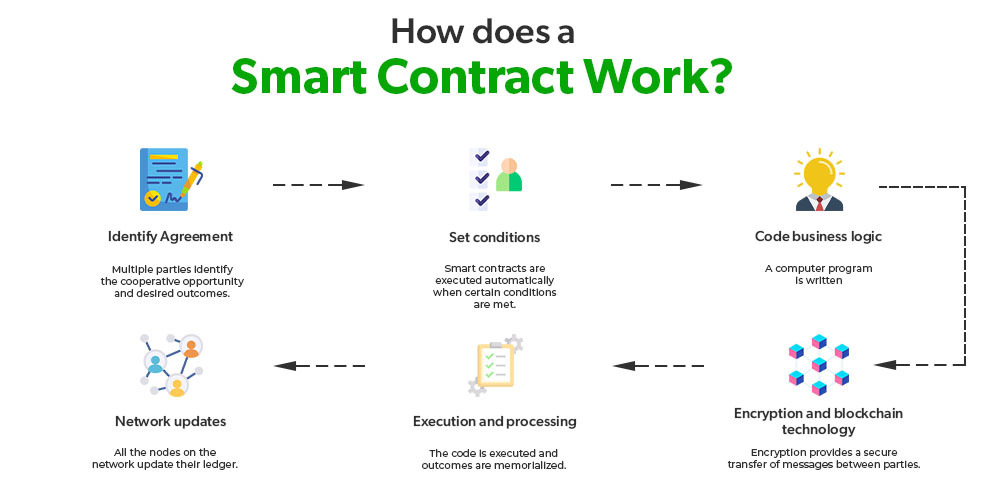
\includegraphics[scale=0.4]{Documentation/figures/smart.png}  % largura percentual
	\caption{Workflow of a Smart Contract, source: \href{https://www.geeksforgeeks.org/smart-contracts-in-blockchain/}{GeeksforGeeks}}
	\label{fig:smartcont}
\end{figure}

Smart Contracts can be applied in many industries, such as healthcare or real estate, but they will be of tremendous importance when it comes to \textit{management} and \textit{voting} on Dharma Network (more detailed at chapter \ref{chap:chap4}).\newline

Smart Contracts in Algorand (layer-1 smart contracts, or ASC1- see figure \ref{fig:algoprimer}) can be of two types: smart contracts and smart signatures.\newline

\textit{Smart Contracts}, also called \textit{Stateful Smart Contracts}, function as state-holding contracts and store on-chain values globally or for individual accounts. They are initiated by stateful smart contract transactions and process the logic within the contract.\newline 
Stateful smart contracts can be linked with payment transactions using Algorand's Atomic transfer capability (see figure \ref{fig:algoprimer}), which allows multiple transactions to be submitted simultaneously. By leveraging this feature, stateful smart contracts can effectively approve or reject a spending transaction based on the logic they contain. The ABI (\textit{Application Binary Interface}) provides a standard method for exposing APIs and encoding/decoding data types for application call transactions \cite{scalgo, scalgo2}.\newline

\begin{figure}[htbp]
	\centering
	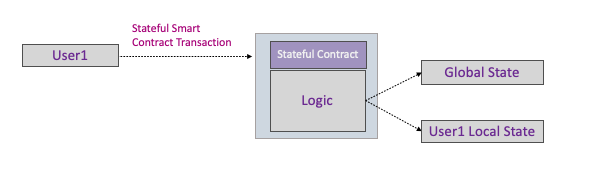
\includegraphics[scale=0.5]{Documentation/figures/stateful.png}  % largura percentual
	\caption{Workflow of a Stateful Smart Contract, source: \href{https://developer.algorand.org/articles/linking-algorand-stateful-and-stateless-smart-contracts/}{Algorand Developer Portal}}
	\label{fig:stateful}
\end{figure}

On the other hand, \textit{Smart Signatures}, also known as \textit{Stateless Smart Contracts}, are primarily used to approve spending transactions with logic. The logic is submitted with a transaction and evaluated by the AVM. If the logic fails, the associated transaction is not executed. They can be signed by a user's signature, a multi-signature or with the logic of a stateless smart contract itself. \newline
Smart signatures can function as accounts similar to other accounts on the blockchain, allowing funds to leave only if the transaction successfully executes the logic within the smart signature. They can also be used for account delegation, where an account signs the smart signature, which can be used later to sign a transaction from the original signer's account\cite{scalgo, scalgo2}.

\begin{figure}[htbp]
	\centering
	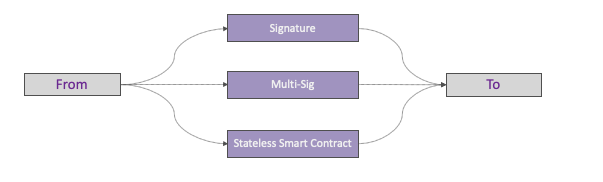
\includegraphics[scale=0.5]{Documentation/figures/stateless.png}  % largura percentual
	\caption{Workflow of a Stateless Smart Contract, source: \href{https://developer.algorand.org/articles/linking-algorand-stateful-and-stateless-smart-contracts/}{Algorand Developer Portal}}
	\label{fig:stateless}
\end{figure}

Both smart contracts and smart signatures are evaluated by the AVM, with access to limited global variables, temporary scratch space and transaction properties. They play different roles in the Algorand ecosystem, with smart contracts providing decentralized application logic and state management, while smart signatures focus on transaction signing and delegation \cite{scalgo, scalgo2}.

\subsubsection{Types of Blockchain}\label{typesofb}

Blockchains can be split into two main groups: permissionless and permissioned. Each one is used depending on the operation to perform \cite{perm_bc}.

\begin{enumerate}
    \item \textbf{Permissioned Blockchain} is ideal for applications requiring role definition and limited access. Users are added or removed based on digital verification or certificates, offering an additional layer of security and privacy compared to public blockchains \cite{bc_types, perm_bc}.

These are implemented by major companies worldwide due to its security features and they're commonly used in supply chain management, contract creation, identity verification and payment verification.

Some of its features are:

\begin{itemize}
    \item \textit{Transparency:} Clear tracking of changes and user actions.
    \item \textit{Data Security:} Complete control over data access and permission management.
    \item \textit{Lack of Anonymity:} Every change is tracked to individual users, promoting accountability.
    \item \textit{Restricted Authority:} Private groups can authorize decisions without centralized control \cite{perm_bc}.
\end{itemize}

    \item \textbf{Permissionless Blockchain}, also known as public blockchain, is a blockchain open to participation without restrictions. It's a decentralized platform with no central authority or administrator, so the transparency of transactions is available to all participants.
It offers open-source development and limited anonymity \cite{bc_types, perm_bc}.


These are commonly used in financial platforms, digital trading, donations and crowdfunding.\newline

Some of its features are:

\begin{itemize}
    \item \textit{Transparent Transactions:} Complete visibility of transactions to all users.
    \item \textit{Open Development:} Accessibility for users to modify and improve the platform.
    \item \textit{Anonymity:} Participants have certain exceptions to privacy while making changes.
    \item \textit{Lack of Central Authority:} No centralized control or authorization required.
    \item \textit{Token Incentives:} Use of tokens and digital assets to encourage participation \cite{perm_bc}.
\end{itemize}

For a further understanding of the difference between them, see table \ref{tab:blockchain-comparison} to see their comparison and table (table \ref{proscons} to check their pros and cons.\newline
\end{enumerate}


Inside the world of permissioned and permissionless blockchains, there's 4 types: \textit{public blockchain}, \textit{private blockchain}, \textit{hybrid blockchain} and \textit{consortium blockchain} (see figure \ref{fig:type})\cite{bc_types}.

\begin{figure}[htbp]
	\centering
	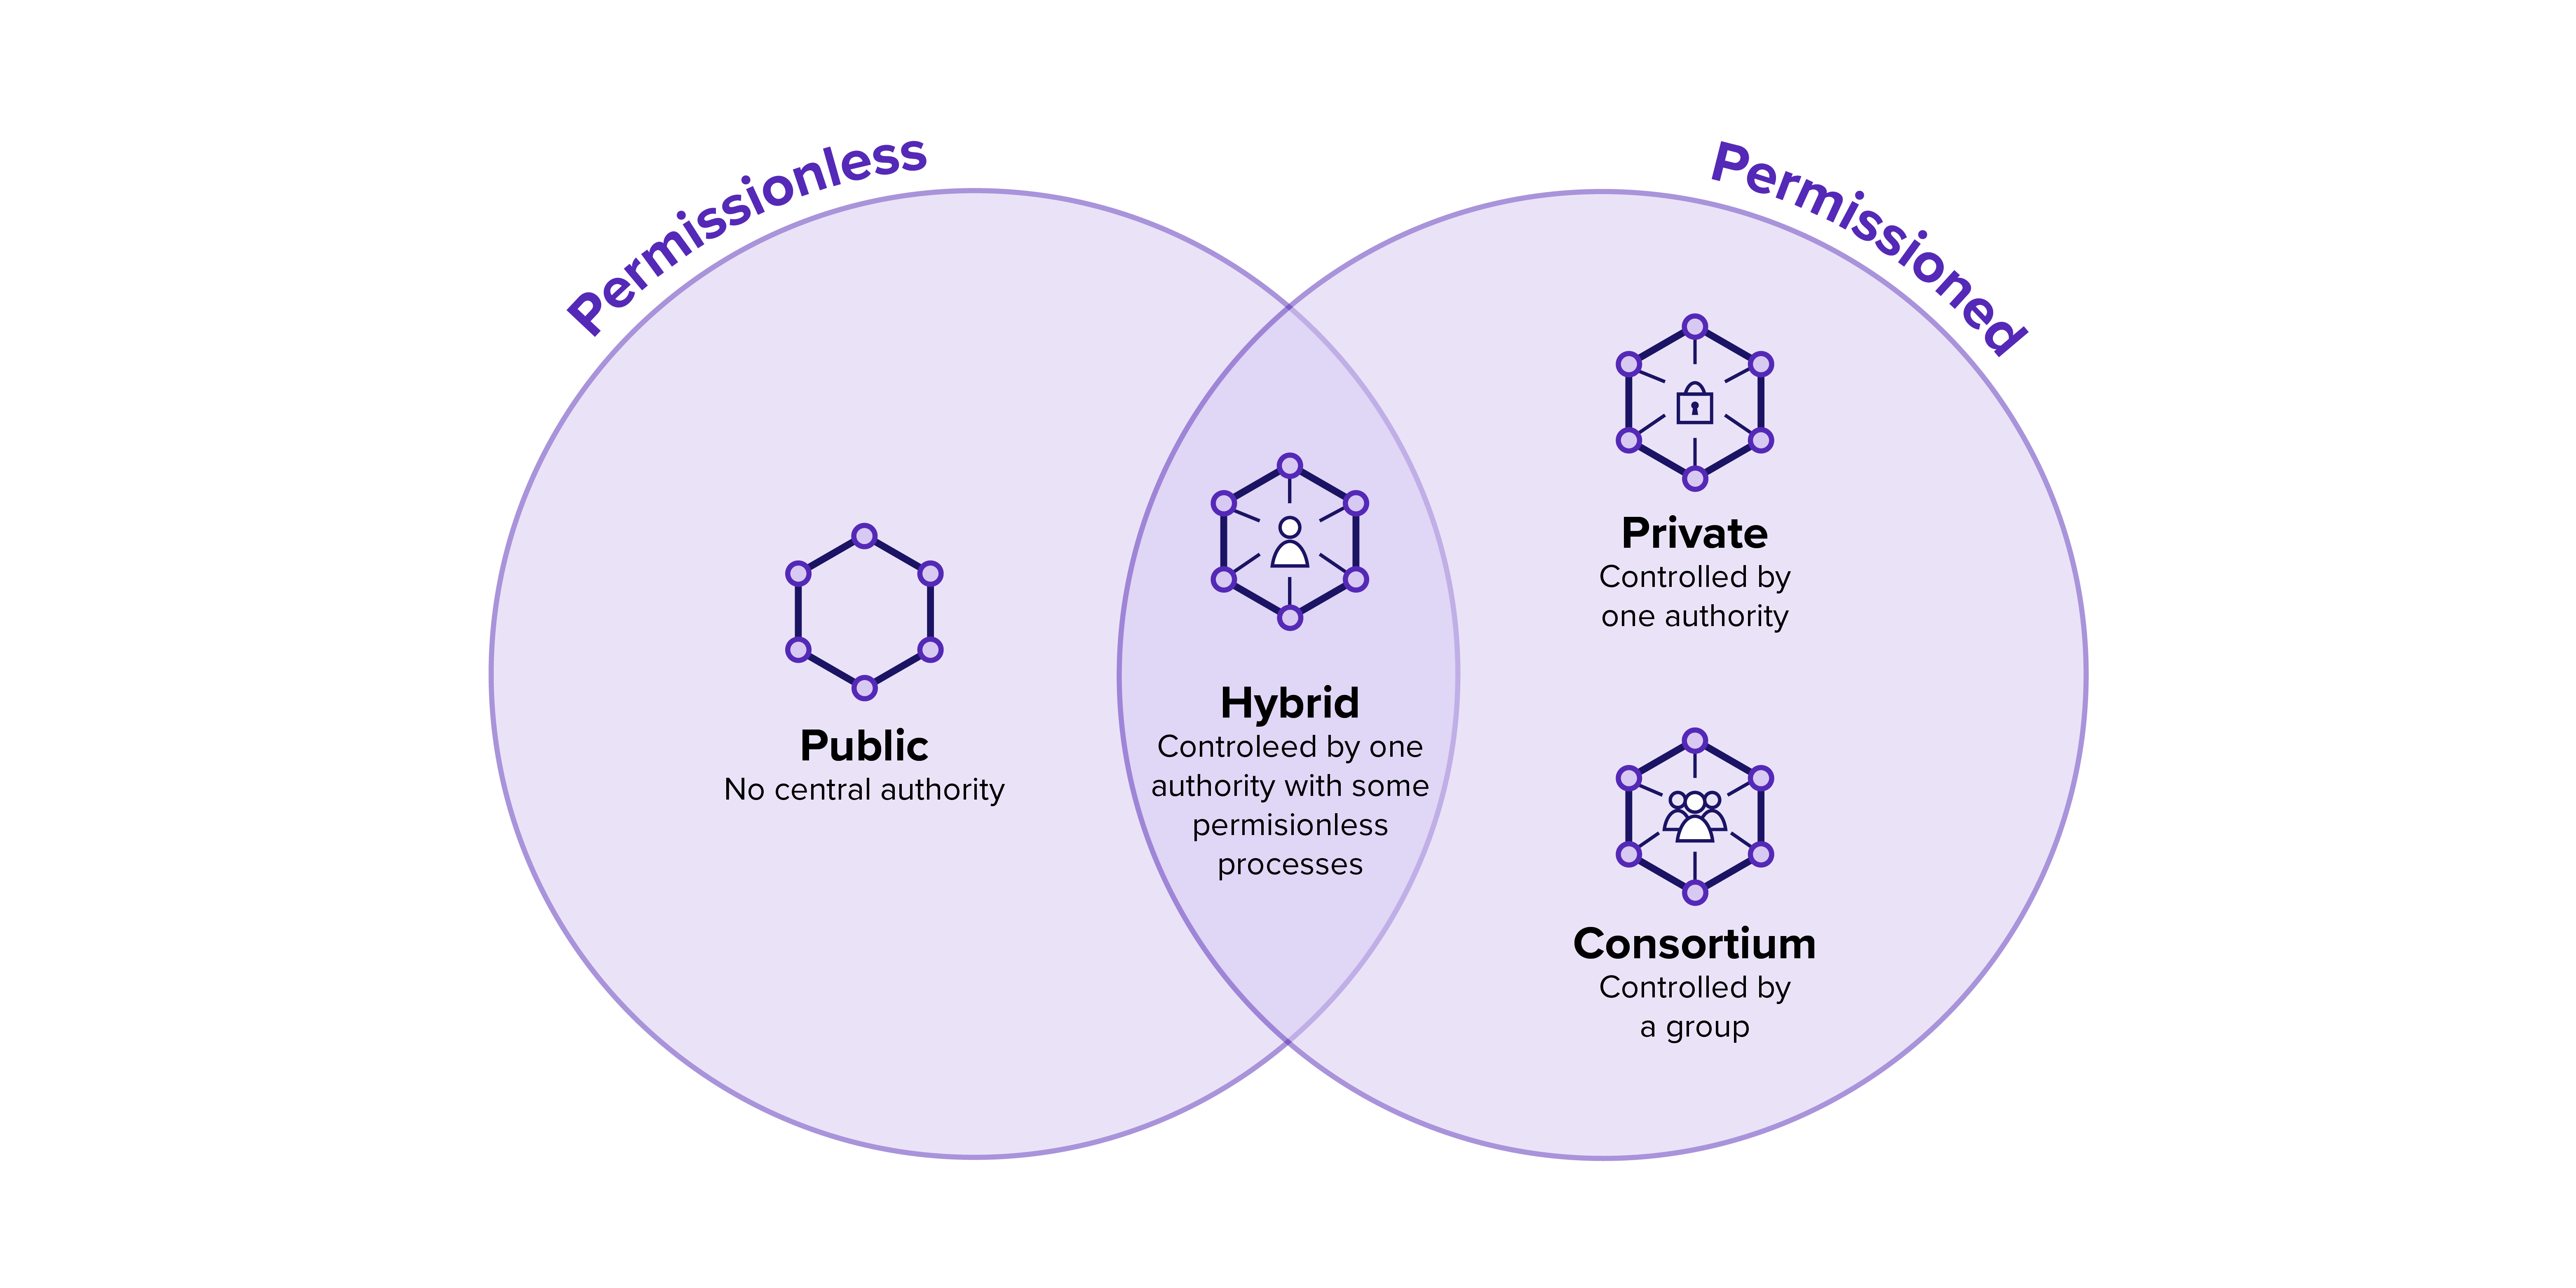
\includegraphics[scale=0.2]{Documentation/figures/perm.png}  % largura percentual
	\caption{Venn Diagram of Blockchain Types, source: \href{https://www.parcl.co/blog/the-4-types-of-blockchain-and-why-you-should-know-the-difference}{Parcl}}
	\label{fig:type}
\end{figure}

\begin{enumerate}
    \item \textbf{Public Blockchain:}

    Public blockchain operates on a permissionless distributed ledger, allowing anyone to join and participate in transactions. The open nature of public blockchains promotes transparency and trust within the user community. Bitcoin, as one of the earliest public blockchains, enabled decentralized transactions accessible to anyone with an internet connection. However, public blockchains face challenges in scalability and privacy, making them more suitable for applications such as voting and fundraising.
    
    \item \textbf{Private (or Managed) Blockchain:}

    Private blockchains operate in closed networks and are managed by organizations. These blockchains provide a higher degree of control and privacy compared to public blockchains. In a private blockchain, access and permissions are restricted, allowing for faster transactions and scalability. Organizations can employ private blockchains to streamline supply chain management, track asset ownership, or facilitate internal voting processes. However, the centralized nature of private blockchains contradicts the decentralized principles of blockchain technology and security may be compromised due to the limited number of nodes.
    
    \item \textbf{Consortium Blockchain:}

    Consortium blockchains, also known as federated blockchains, combine elements of both public and private blockchains. These blockchains are controlled by multiple organizations, striking a balance between transparency and privacy. Consortium blockchains offer scalability, security, and efficient governance structures. Use cases for consortium blockchains include banking and payment systems, research collaborations and supply chain management. However, the integrity of the member organizations can impact the network's effectiveness, and legal and regulatory factors may influence its operations.
    
    \item \textbf{Hybrid Blockchain:}

    A hybrid blockchain combines features of both private and public blockchains, catering to organizations that require the benefits of both worlds. It allows for private and secure transactions while still being part of a public network. Hybrid blockchains offer flexibility in adjusting rules and providing privacy as needed. Real estate, retail, and highly regulated industries can leverage hybrid blockchains to improve process efficiency and comply with strict regulations. However, the lack of full transparency and the complexity of transitioning to hybrid blockchains are notable considerations.
\end{enumerate}

Understanding the characteristics of each type enables organizations to make informed decisions when adopting blockchain technology, aligning with their goals and industry requirements.

\subsubsection{Algorand Blockchain}\label{algo_bc}

Dharma Network is built on top of Algorand blockchain, as previously mentioned. 

The following figure \ref{fig:algoprimer} mentions four essential components that were and will continuously be mentioned in the course of this paper:

\begin{figure}[htbp]
	\centering
	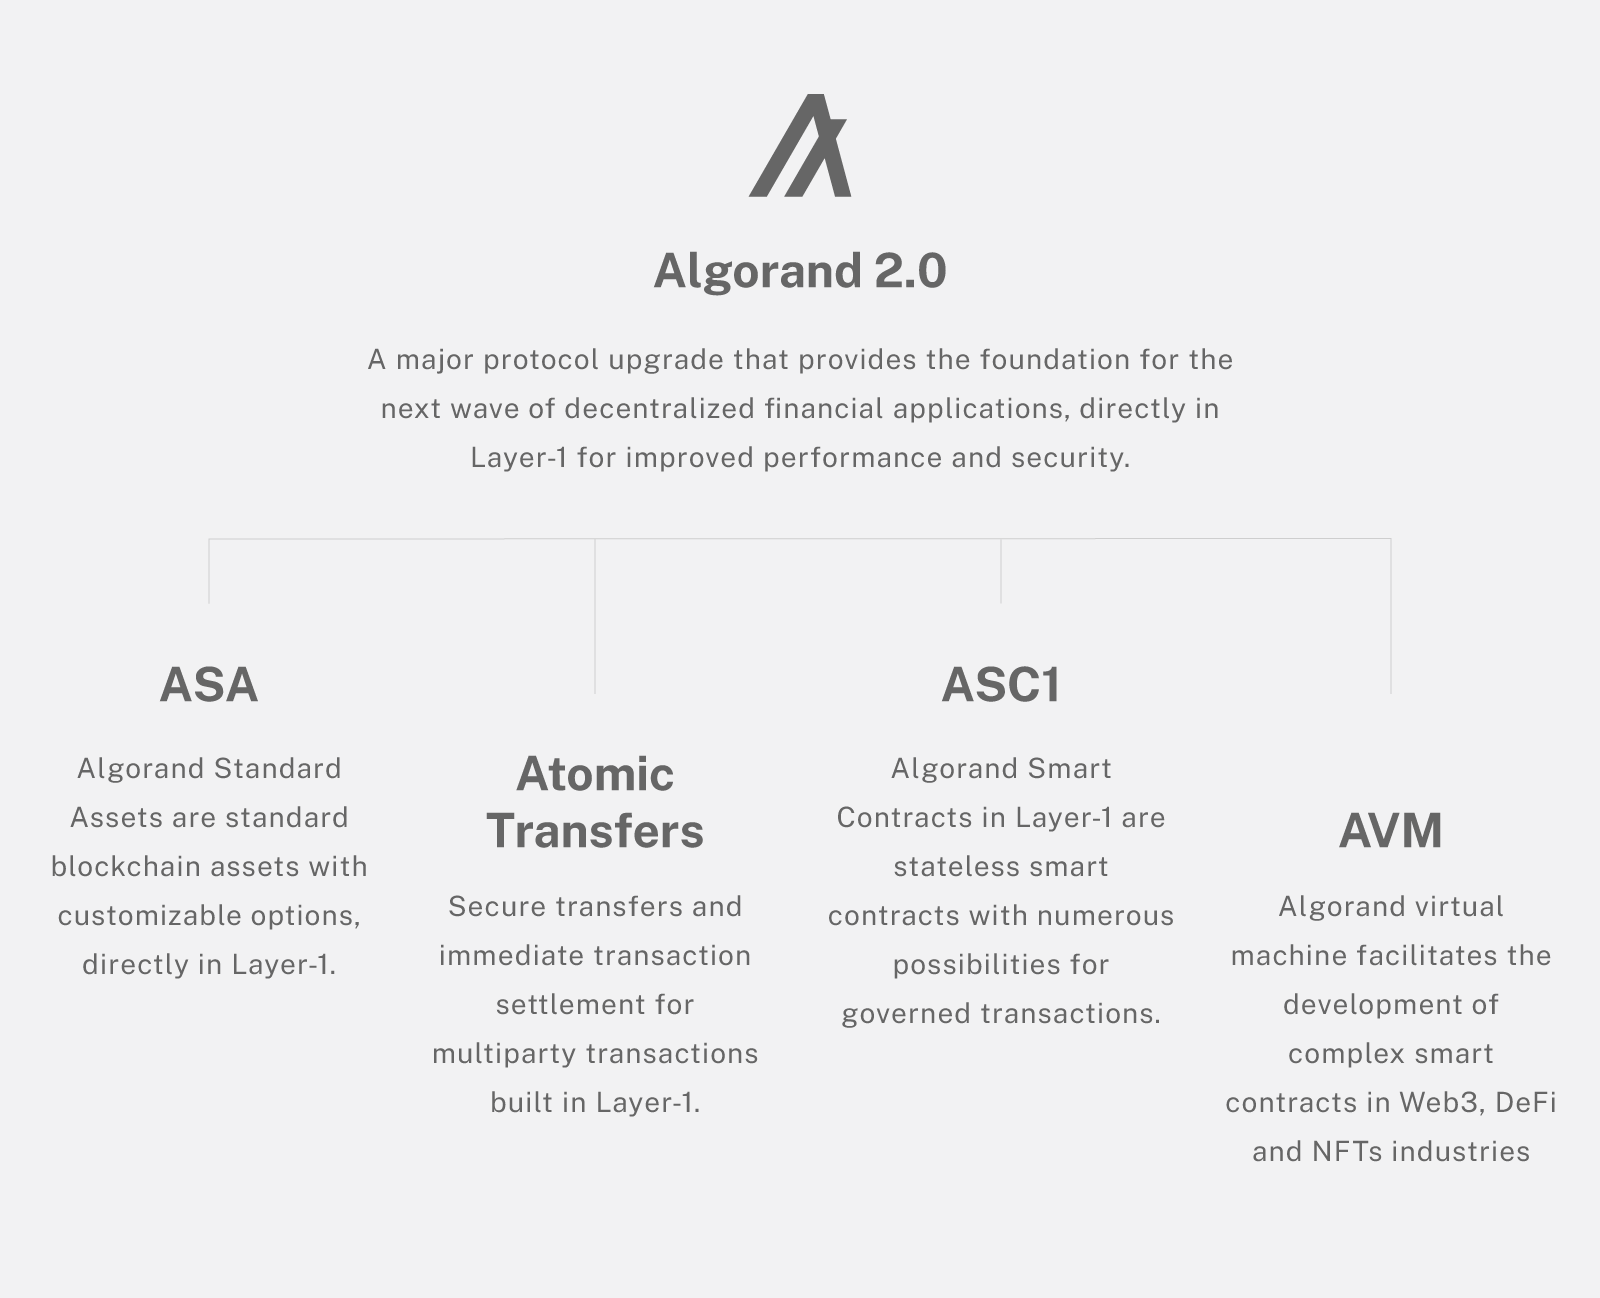
\includegraphics[scale=0.2]{Documentation/figures/Algorand_primer_content_10 (1).png}  % largura percentual
	\caption{Algorand (ALGO) Research Primer, source: \href{https://21shares.com/research/algorand-research-primer}{21Shares}}
	\label{fig:algoprimer}
\end{figure}

\begin{tcolorbox}[colback=white!20!white,colframe=red!80!black,rounded corners]
\danger An important feature to mention is that Yarilabs created their own Algorand SDK\footnotemark, written in Elixir: the \textit{Algodex}.\newline

Algodex is specifically designed to interact with the Algorand blockchain. It provides developers with a framework and a collection of functions and resources to facilitate the integration of Algorand's features and capabilities into their Elixir-based applications.\newline

By using Algodex, developers can leverage the functionalities of the Algorand blockchain, such as creating and managing accounts, sending and receiving transactions, querying blockchain data, interacting with smart contracts and more. The SDK abstracts away some of the complexities of interacting with the Algorand blockchain, making it easier and more efficient for developers to build Algorand-powered applications using the Elixir programming language.\danger
\end{tcolorbox}

\footnotetext{An SDK (Software Development Kit) is a set of tools, libraries, and documentation that simplifies the development of applications for a specific platform or technology.}

The consensus mechanisms mentioned on section \ref{cons.mec} are incredibly powerful, but Algorand Blockchain takes advantage of another mechanism: Pure Proof-of-Stake (PPoS).

As seen on \href{https://algorand.com/technology/algorand-protocol}{Algorand's technology page}, its consensus mechanism is permissionless (see \ref{typesofb}) and PURE PROOF OF STAKE™.\newline

Algorand's PPoS protocol incorporates Byzantine consensus\footnote{The corresponding Byzantine Consensus is not exactly the same as seen on section \ref{cons.mec}, since there's some variations of the algorithm. For a further understanding, please read paper \cite{algo}}, where the influence of each user on the selection of a new block is directly proportional to their stake (number of tokens) in the system. Random and secret selection of users to propose blocks and vote on block proposals ensures fairness and security. Unlike other approaches, where a small subset of the economy determines the security of the whole economy, Algorand's PPoS ties the security of the entire system to the honesty of the majority. This approach ensures that malicious users holding a small fraction of the money cannot harm the entire network, making Algorand more resilient \cite{alg}.\newline

\textbf{How does PPoS work?} \cite{alg, algo, ppow}\newline

In Algorand, participation is open to all token holders, which \textit{is what makes it a pure proof-of-stake (PPoS) protocol}. Each participant holds a certain number of Algorand tokens (ALGOs) in their wallet, allowing them to engage in the consensus protocol and contribute to the network's security and operations.\newline

\textbf{Protocol Participation:}
To participate in the protocol, users generate and register a participation key, separate from their spending keys, ensuring the security of their tokens even if their participating node is compromised. With the participation key, users can propose and vote on blocks, actively contributing to the consensus process.\footnote{This defines the Gossip protocol shown in figure \ref{fig:algo, fig:algoflow}.}\newline

\textbf{Block Proposal:}
During each round of the consensus protocol, a subset of participants is randomly selected to propose a new block. The selection process is based on the number of tokens held by each participant, giving those with a larger stake a higher probability of being chosen as block proposers. This fair and secure selection mechanism ensures that the consensus protocol is inclusive and that participants with a significant stake have a greater influence on block proposal.\newline

\textbf{Block Validation:}
After a block is proposed, a different subset of participants is randomly chosen to validate the block. Validators carefully examine the proposed block for correctness and legitimacy. The selection of validators is determined using a verifiable random function (VRF), ensuring a decentralized and unbiased validation process. Validators play a crucial role in maintaining the integrity of the blockchain by verifying proposed blocks.\newline

\textbf{Soft Vote:}
In the soft vote phase, nodes run the VRF for each participating account they manage to determine if they have been chosen to be part of the soft vote committee. If selected, these accounts contribute weighted votes based on the number of ALGOs they hold. The soft vote committee filters the block proposals down to one by voting to confirm the block with the lowest VRF output calculated at the timeout. These votes, along with the VRF proof, are shared with other nodes, and each node validates the committee membership VRF proof before adding it to the vote tally. Once a quorum is reached for the soft vote, the process advances to the certify vote step.\newline

\textbf{Certify Vote:}
Following the soft vote, a new committee is formed to check the block proposal that received the soft vote for potential issues such as overspending or double-spending. If the block is deemed valid, the committee proceeds to vote on certifying the block. Similar to the soft vote, each node selects a committee from its managed accounts and sends their votes. These votes are collected and validated by each node until a quorum is reached, indicating consensus. Once the block is certified, it is considered final and added to the blockchain.\newline

\textbf{Block Confirmation:}
After the block is certified by a sufficient number of participants, it is confirmed and added to the blockchain. The confirmation process enhances the finality of the block, making it highly unlikely to be reverted. This immutability strengthens the integrity and reliability of the Algorand blockchain.\newline

\textbf{Consensus Agreement:}
Algorand achieves consensus agreement through a decentralized Byzantine Agreement (BA) protocol called Binary Byzantine Agreement (BBA). This protocol enables participants to collectively agree on the block proposal and validation outcome, even in the presence of malicious actors or network issues. By leveraging BBA, Algorand ensures a robust and secure consensus mechanism.\newline

\textbf{Fast and Scalable Block Production:}
Algorand's consensus mechanism enables fast block production, with a new block added to the blockchain approximately every 4.5 seconds. This high throughput rate ensures scalability, enabling the Algorand network to handle a large number of transactions efficiently. The combination of random selection through VRF, the weighted voting system based on stake, and the use of BBA protocol contribute to the fast and secure block production process.\newline

By incorporating the principles of pure proof-of-stake, random selection for block proposal and validation, soft and certify votes, and Byzantine Agreement protocols, Algorand establishes a robust and decentralized consensus mechanism. This approach allows Algorand to provide a high-performance blockchain platform that is secure, scalable and inclusive for all token holders.\newline

Figures \ref{fig:algo} and \ref{fig:algoflow}can be used as an example of what was just explained:\newline

\begin{figure}[htbp]
	\centering
	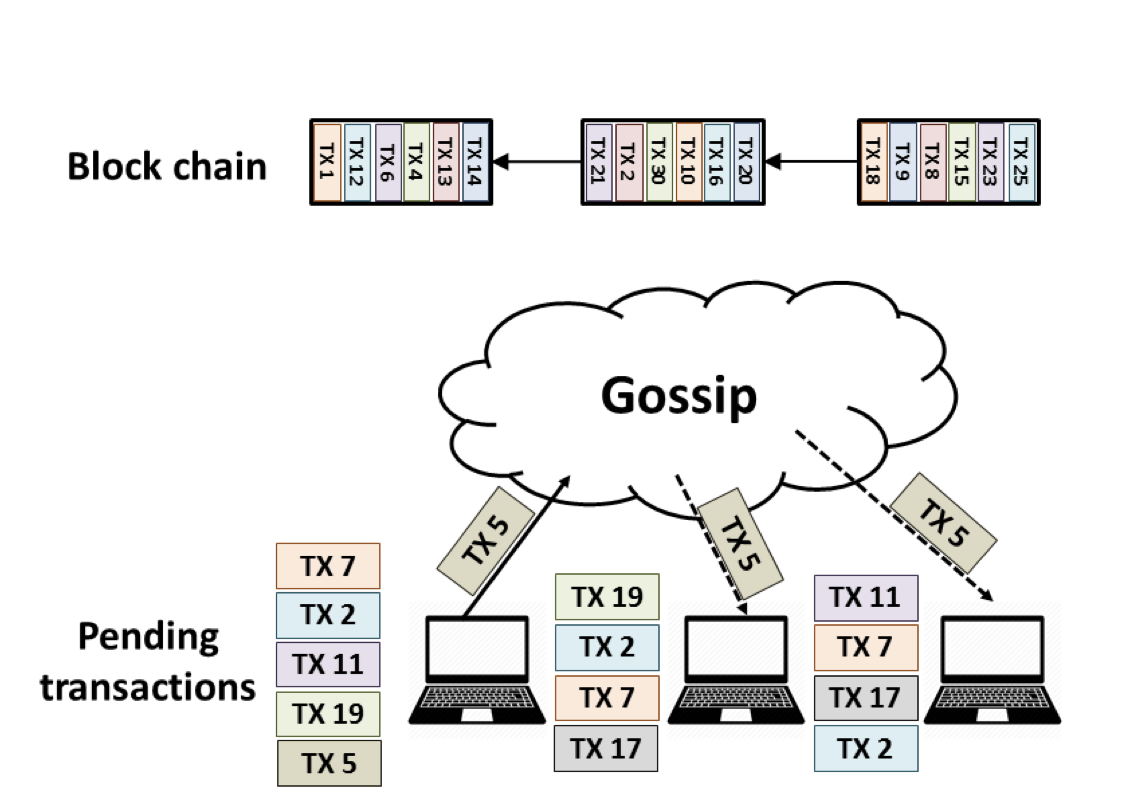
\includegraphics[scale=0.4]{Documentation/figures/algorand_workflow.png}  % largura percentual
	\caption{Transaction Flow in Algorand, source: \href{https://people.csail.mit.edu/nickolai/papers/gilad-algorand-eprint.pdf}{MIT}}
	\label{fig:algo}
\end{figure}

\begin{figure}[htbp]
	\centering
	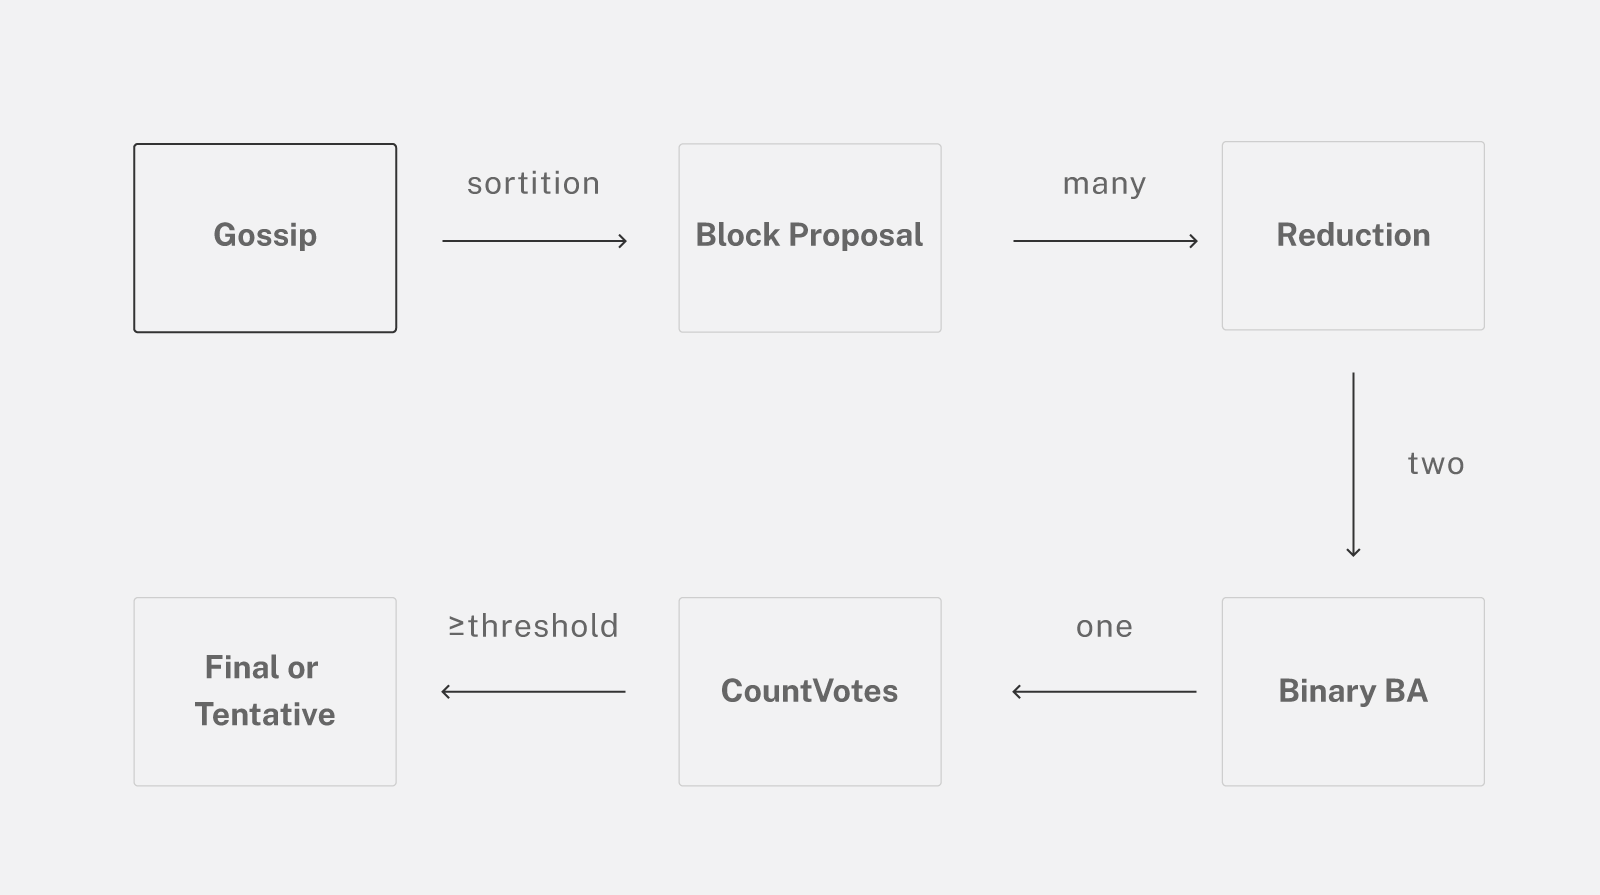
\includegraphics[scale=0.2]{Documentation/figures/Algorand_primer_content_04.png}  % largura percentual
	\caption{Transaction Flow in Algorand, source: \href{https://21shares.com/research/algorand-research-primer}{21Shares}}
	\label{fig:algoflow}
\end{figure}

\textbf{Advantages over Proof-of-Work (PoW):}\newline

PoW, the consensus mechanism used by Bitcoin and Ethereum, suffers from several limitations. It is highly resource-intensive, requiring specialized hardware and significant energy consumption. In contrast, Algorand's PPoS eliminates the need for resource-intensive mining, making participation accessible to all users without specialized equipment or excessive energy consumption. This reduces barriers to participation and fosters a more inclusive and sustainable network.\newline

Furthermore, PoW systems often lead to a concentration of power in mining pools, risking centralization and potential manipulation. Algorand's PPoS ensures that malicious users gain no advantage by splitting their stake or pooling resources, as influence is solely based on stake proportion. This enhances decentralization and security within the network, eliminating the vulnerability associated with concentrated power.\newline


\textbf{Scalability and Finality:}\newline
Scalability is a critical factor for blockchain protocols aiming to serve a global economy. PoW systems face challenges with block propagation, resulting in slower transaction processing times. In contrast, Algorand's PPoS protocol boasts low computation and communication overhead, enabling rapid block propagation within seconds. This scalability allows Algorand to sustain a high transaction rate, making it suitable for large-scale adoption and real-world financial applications.\newline

Additionally, Algorand's PPoS eliminates the occurrence of forks, ensuring transaction finality. In PoW systems, forks can cause uncertainty and delays, requiring multiple block confirmations to ensure a transaction is valid. Algorand's single block certification mechanism ensures that once a block is added to the chain, transactions within it are considered final, providing immediate transaction certainty and enhancing user confidence.\newline

\subsection{DHARM- Dharma Network's token}

DHARM is the main token of Dharma Network's DApp. It's a stable and mineable token, mined with Proof-of-Real-Work, which is executed by an user on a specific project. It has 8 decimals just like Bitcoin and it's smallest unit is called \textit{nanoDharm} \cite{dharma}.

\begin{equation}
    1 nanoDharm = 0.0000 0001 Dharm
\end{equation}

\textit{Proof-of-Real-Work} shares similarities with the Proof-of-Work (PoW) mechanism used in blockchain networks like Bitcoin. However, there is one major difference: the computational effort expended in DHARM's mining process is directly linked to real-world activities or transactions, distinguishing it from the abstract computational puzzles typically associated with PoW.\newline

Some relevant \textit{blockchain components of Dharma Network} are the following:

\begin{itemize}
    \item \textit{Minter} - TEAL stateless escrow contract that will own the unminted tokens (will be the new DHARM reserve account)
    \item \textit{Dharma Scriber} - TEAL stateful smart contract that miners need to opt-in. Scriber writes to users local-state how much Dharm they mined, bonus mining rewards and verification data. It’s also responsible to reset the local-state when users claim their DHARM successfully on an atomic swap with the minter
    \item \textit{Dharma Oracles} - writes DHARM blocks information into the Algorand Blockchain. The exchange rates for DHARM/ALGO are also published by the oracle
    \item \textit{Organization Escrows} - Every organization has its own smart contract to hold the funds of the funding rounds
    \item \textit{Rewards Calculator} - responsible to calculate mining rewards. Calls the Dharma Scriber to write rewards to users local-state
    \item \textit{Treasury Account (dharma.algo)} - receives the funds from the organization escrows contracts when a funding round is closed successfully \cite{dharma}.
\end{itemize}

\textbf{DHARM's mining process}\newline

DHARM's mining process is implemented in a secured and decentralized manner called ASA (Algorand Standard Asset).\newline

ASA is an on-chain asset that benefit from the same level of security and ease of use as Algo\footnote{Algo is Algorand's native utility token.}. With the help of these, such things as stablecoins, loyalty points and system credits can be represented. Single assets, such as a deed for a house or collectable items, can also be represented. ASAs have a wide range of use cases, allowing for the representation of both fungible and non-fungible assets with varying degrees of control. \newline

ASAs offer several important concepts that developers need to understand when working with them. Some of those concepts are:

\begin{enumerate}
    \item \textbf{ASA Transaction Types and User Flows:}

    There are three primary transaction types associated with ASAs: \textit{AssetConfigTxn (acfg)}, \textit{AssetFreezeTxn (afrz)}, and \textit{AssetTransferTxn (axfer)}. Each transaction type serves a specific purpose and, combined with different parameter specifications, supports seven primary user flows:

    \begin{itemize}
        \item \textit{Asset Creation:} Creating a new asset on the Algorand blockchain.
        \item \textit{Asset (Re-)Configuration:} Modifying the configuration of an existing asset, such as changing its name or total supply.
        \item \textit{Asset Freezing:} Enabling the freezing of assets, allowing certain accounts to control the ability to trade the asset.
        \item \textit{Asset Destruction:} Removing an existing asset from the blockchain.
        \item \textit{Asset Transfer:} Transferring assets between accounts.
        \item \textit{Asset Revocation:} Revoking assets from a specific account and transferring them to another account.
        \item \textit{Asset Opt-In:} Allowing an account to receive a new type of asset.
    \end{itemize}

    Each one of these transaction types and user flows is more detailed in figure \ref{fig:asa}:

    \begin{figure}[htbp]
	   \centering
	   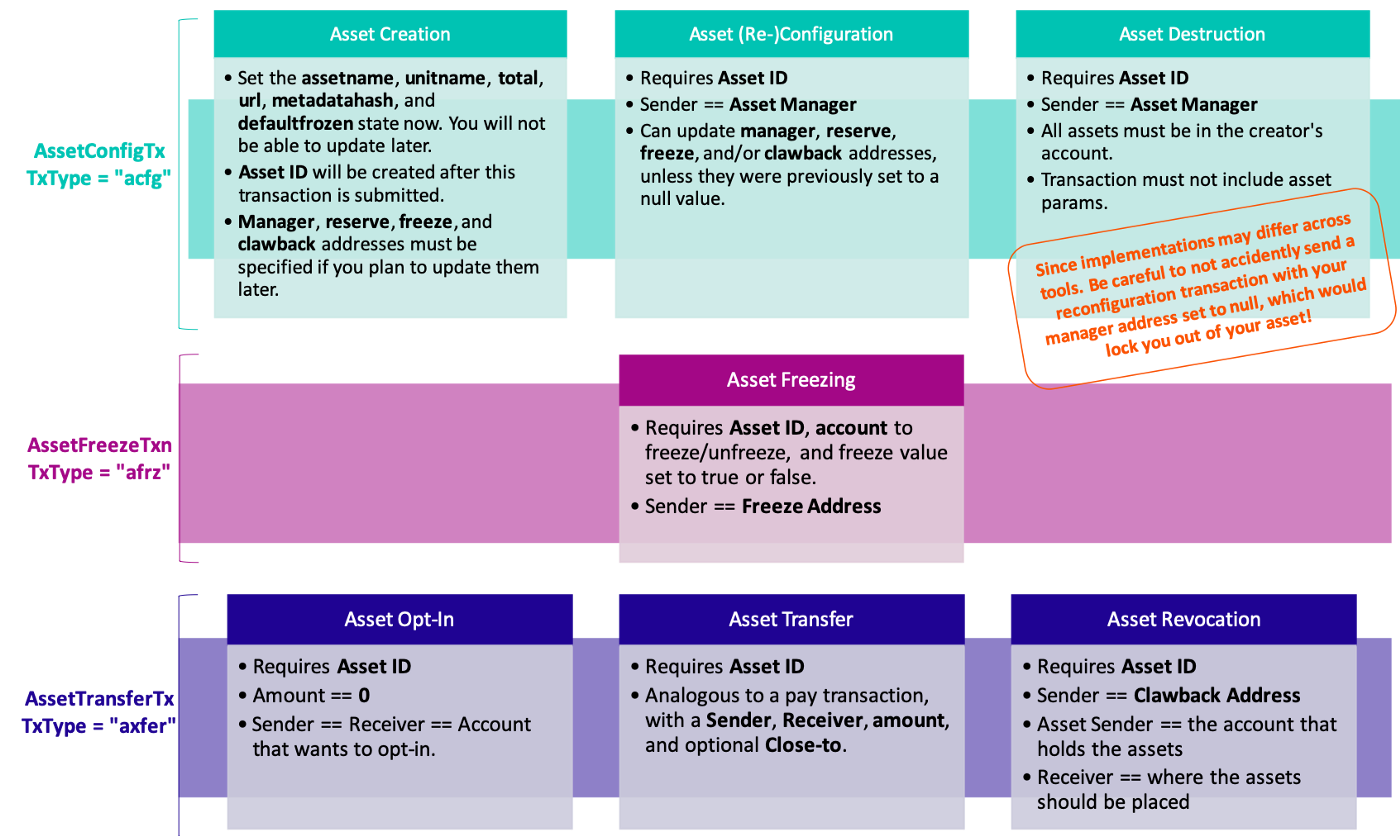
\includegraphics[scale=0.2]{asa}  % largura percentual
	   \caption{ASA Transaction Types, source: \href{https://developer.algorand.org/articles/algorand-standard-assets/}{Algorand's Developer Portal}}
	   \label{fig:asa}
    \end{figure}

    
    \item \textbf{Asset Opt-Ins:}

    To receive a new type of asset, an account must opt-in. This process involves sending a 0-amount transfer of the desired asset from and to the account itself. By opting-in, a holding for the new asset is created in the account, enabling others who own that asset to transfer it to the account.

    \item \textbf{Minimum Balance Requirement:}

    Every Algorand address on the ledger must maintain a minimum balance of 100,000 microAlgos. When an account opts-in to receive an ASA, the minimum balance increases by 100,000 microAlgos. For example, if an account opts-in to receive two different ASAs, the minimum balance will be 300,000 microAlgos (100,000 microAlgos x 2 ASAs + 100,000 microAlgos for the native Algo).


    \item \textbf{Freeze Assets:}

    Upon asset creation, it is possible to specify a freeze address and a defaultfrozen state. Setting the defaultfrozen state to true requires the corresponding freeze address to issue unfreeze transactions, allowing trading of the asset to and from specific accounts. This feature can be useful for implementing checks like KYC/AML requirements. Conversely, setting the defaultfrozen state to false allows anyone to trade the asset, and freeze transactions can be issued by the freeze address to disallow trading for specific accounts. To ensure asset holders that the asset will never be frozen, the defaultfrozen state can be set to false, and the freeze address can be set to null or an empty string.

    \item \textbf{Revoke Assets:}

    ASAs also offer the ability to revoke assets from specific accounts using a clawback address. If specified, the clawback address can revoke the asset from any account and transfer it to another account that has previously opted-in. This feature is valuable in situations where asset holders breach certain terms or conditions established for the asset. Similar to freezing, the clawback address can be set to null if it is desirable to ensure that asset revocation is not possible.

    
\end{enumerate}



ASAs are supported at the protocol level on the Algorand Blockchain. When an ASA is created, the entire supply is automatically generated and becomes immediately available. However, ASAs do not natively support incremental mining.\newline

To address this, the Dharma Network has implemented a stateless escrow contract called the Minter. The Minter acts as the sole entity responsible for transferring Dharm tokens to miners. Instead of having a reserve account controlled by a central entity, the Minter holds the unminted tokens and ensures their secure distribution.

To request Dharm tokens from the Minter, an account that has opted into Dharm must create a transaction as part of a grouped atomic transaction. This transaction must include:

\begin{enumerate}
    \item A request to the Minter for Dharm tokens, accompanied by proof in the local state that the user is entitled to receive those tokens.
    \item A call to the Dharma Scriber smart contract to reset the state.
\end{enumerate}

Algorand supports atomic transactions (see figure \ref{fig:algoprimer}), meaning that if any of the transactions within a grouped atomic transaction fails, all of them fail. Therefore, the Minter checks that the miners have used a group transaction, are eligible to receive Dharm tokens, and that the Scriber contract was successfully called. This ensures the integrity and correctness of the mining process.\newline

The use of atomic transactions, in combination with the Proof of Real Work mechanism described in the additional information, adds an extra layer of security to the mining process. The activity transactions related to mining are stored on an immutable chain of blocks, making the entire mining process secure and publicly verifiable.\newline


\textbf{Dharma Network's DAO:}\newline

The Dharma Network embraces a decentralized approach to governance and recognizes the importance of establishing a strong foundation to support its operations. To this end, the Dharma Network Foundation will be set up to provide legal support in the formation of a \textit{Decentralized Autonomous Organization} (DAO) for DHARM \cite{dharma}.\newline

A DAO, or Decentralized Autonomous Organization, is a concept that leverages blockchain technology to create an organization that operates in a decentralized and autonomous manner. It is designed to eliminate the need for traditional centralized management structures and instead relies on smart contracts and distributed consensus mechanisms to govern and execute its operations.\newline

The purpose of a DAO is to enable a group of individuals or participants to collectively make decisions, manage resources and execute actions without relying on a central authority. By leveraging blockchain's transparency, immutability and decentralized nature, a DAO aims to create a trustless and efficient system that operates based on predefined rules and algorithms.\newline

The key features and purposes of a DAO include \cite{dao, dao2, dao3}:

\begin{itemize}
    \item \textit{Decentralization:} A DAO operates on a decentralized network, typically a blockchain, where no single entity or individual has control over the organization's operations or decision-making. Instead, decision-making power is distributed among participants based on predetermined rules.
    \item \textit{Autonomy:} A DAO is designed to be autonomous, meaning it can perform predefined actions and execute transactions without requiring direct human intervention. Smart contracts, which are self-executing agreements with the terms of the agreement directly written into code, enable this autonomy.
    \item \textit{Governance:} DAOs allow participants to collectively make decisions through voting mechanisms. Each participant typically has voting power proportional to their stake or ownership in the organization, allowing for democratic decision-making processes.
    \item \textit{Resource Management:} DAOs can manage and allocate resources based on predefined rules and algorithms encoded in smart contracts. This can include managing and distributing funds, assets, or tokens held by the organization.
    \item \textit{Transparency:} As DAOs are built on blockchain technology, all transactions, decisions, and changes to the organization's state are recorded on the public ledger. This transparency ensures that all participants can audit and verify the actions and transactions within the organization.
    \item \textit{Trustlessness:} DAOs aim to eliminate the need for trust between participants by relying on the transparency and immutability of blockchain technology. All actions and operations are recorded on the blockchain, and smart contracts execute based on predefined rules, removing the need for trust in individual participants.
\end{itemize}

The overall difference of DAO and traditional organizations is represented on figure \ref{fig:dao}:

    \begin{figure}[htbp]
	   \centering
	   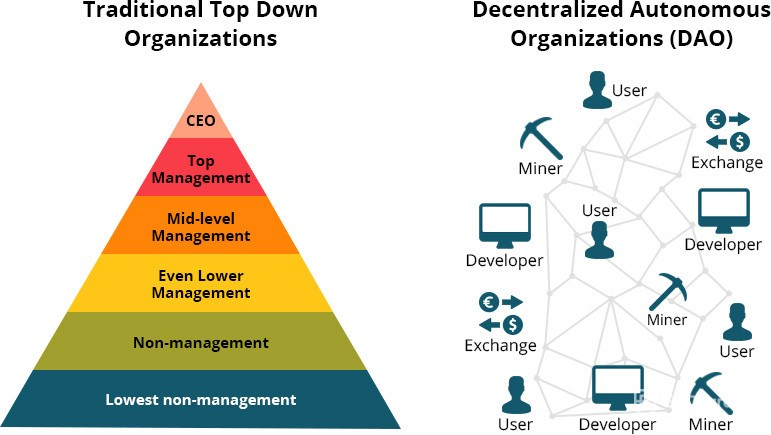
\includegraphics[scale=0.4]{Documentation/figures/dao.png}  % largura percentual
	   \caption{Difference between Traditional Organizations and Decentralized Autonomous Organizations, source: \href{https://academy.moralis.io/blockchain-guides/beginners-guide-how-to-create-a-dao}{Moralis Academy}}
	   \label{fig:dao}
    \end{figure}

The Dharma Network DAO will be the governing body of the ecosystem, allowing all Dharm token holders to participate in the decision-making process through voting on DAO proposals. This model draws inspiration from the successful implementation of Algorand Governance. By granting token holders voting rights, the DAO ensures that decisions are made in a democratic and inclusive manner, reflecting the collective will of the community.\newline

The responsibilities of the Dharma DAO will encompass various aspects of the network's operations. These include determining which liquidity pools to create, managing liquidity by adding or removing assets, adjusting bonus mining rewards, setting limits for mining activities, and distributing fees. The DAO will play a crucial role in shaping the ecosystem by making informed decisions on these matters.\newline

As the project progresses and achieves a phase of high liquidity, the Dharma DAO will have the ability to open grants for projects that align with the goals and values of the DAO and the Dharma Network as a whole. These projects would need to meet specific criteria, such as having automated activity tracking and bringing value to the ecosystem and the world at large. By providing funding opportunities to promising projects, the DAO aims to foster innovation and collaboration within the Dharma Network.\newline

The funding rounds initiated by the Dharma DAO (DAO funding round) will introduce a unique approach to collateralization. Unlike other funding rounds that require full collateralization, DAO funding rounds may adopt a partial collateralization scheme, such as 25\%/ 75\%, 50\%/ 50\% or 0\%/ 100\%. In these rounds, projects seeking funding will contribute a portion of the collateral and the remaining portion will be granted in mining rewards based on automated activity tracking. This innovative funding mechanism aims to incentivize project participation and align the interests of the project with the overall success of the Dharma Network \cite{dharma}.\newline

It is important to note that the concept of the Dharma DAO and its funding mechanisms will be further developed and detailed in the future. As the Dharma Network evolves and matures, the DAO will continue to play a crucial role in shaping the direction of the ecosystem, promoting collaboration and supporting projects that contribute to the growth and development of the Dharma Network.\newline

\section{Existing Solutions}

While the DeFi landscape is constantly evolving, Dharma Network stands out as a unique solution that combines the power of the Algorand blockchain with innovative mining mechanisms. Existing solutions often rely on centralized systems or lack the level of transparency and decentralization offered by Dharma Network.\newline

However, let's take a look to projects that might have some similarities with Dharma Network.\newline

There are many DAOs based on Algorand, such as \href{https://algorand.com/pt/ecosystem/use-cases/staker-dao}{StakerDAO}, \href{https://algodao.fi}{AlgoDAO} and \href{https://www.algorand.foundation/news/kinn-grant-award}{Kinn DAO}. 

\subsection{Pi Network}

\href{https://minepi.com}{\textit{Pi Network}} is a mobile app-based project that allows users to mine a native cryptocurrency called \textit{Pi} by simply interacting with the app on a daily basis. Similar to Dharma Network, \textit{Pi Network} aims to create a decentralized network of users and incentivize their participation through mining activities. 

\subsection{Steemit}

\href{https://steemit.com}{\textit{Steemit}} is a blockchain-based social media platform that allows users to create and share content while earning rewards in the form of the platform's native cryptocurrency called \textit{STEEM}. Users can contribute by creating blog posts, articles, and other forms of content, and their contributions are rewarded based on the engagement and popularity of their content.\newline

The platform uses a consensus algorithm called \textit{Delegated Proof of Stake} (DPoS), where users can "mine" or earn \textit{STEEM} tokens by staking their existing tokens and participating in the block validation process. Users with more stake have a higher probability of being chosen as block validators and earning rewards.\newline

In addition to earning rewards through content creation and mining, Steemit also has a voting system where users can upvote or downvote content they find valuable or not. These votes not only determine the visibility and popularity of the content but also contribute to the rewards received by the content creators.\newline

Steemit offers a unique way for users to earn cryptocurrency by participating in the platform's activities and engaging with the community. It combines social media features with blockchain technology, creating an incentivized ecosystem where users are rewarded for their contributions \cite{steemit}.\newline

\subsection{Brave Browser}

\textit{Brave Browser} is a privacy-focused web browser that incorporates blockchain technology and a token economy to reward users for their attention and engagement with online advertisements. The browser blocks unwanted ads and trackers by default, providing a faster and more secure browsing experience.\newline

Brave Browser introduces the \href{https://brave.com/brave-rewards/}{\textit{Basic Attention Token}} (BAT) as its native cryptocurrency. Users have the option to opt-in to view privacy-respecting ads while using the browser. When users choose to view these ads, they are rewarded with BAT tokens. The rewards are distributed based on user attention and engagement with the ads, ensuring a fair compensation model.\newline

Additionally, \textit{Brave Browser} allows users to support their favorite content creators directly through BAT token contributions. Users can allocate a portion of their earned BAT tokens to the websites and content creators they appreciate, providing an alternative monetization model for online content.\newline

By integrating blockchain technology and a token-based economy, \textit{Brave Browser} creates a decentralized ecosystem where users are incentivized to engage with advertisements and support content creators, all while maintaining their privacy and control over their data.\newline

\subsection{Gitcoin}

\href{https://www.gitcoin.co}{\textit{Gitcoin}} is a platform that connects developers with open-source projects and provides a way for them to earn rewards for their contributions. It is built on the Ethereum blockchain and utilizes smart contracts to facilitate transparent and incentivized collaboration within the open-source community.\newline

Key features of \textit{Gitcoin} include \cite{gitcoin}:

\begin{itemize}
    \item \textit{Funding Open-Source Projects:} Gitcoin enables individuals and organizations to financially support open-source projects they find valuable. Through the platform, users can contribute funds to specific projects or initiatives they wish to support.
    \item \textit{Bounties:} Gitcoin allows project maintainers to create bounties for specific tasks or issues within their projects. Developers can then choose to work on these bounties and receive rewards upon successful completion. This incentivizes developers to contribute their skills and expertise to the projects that interest them.
    \item \textit{Hackathons and Grants:} Gitcoin hosts online hackathons and facilitates grants to support the development of new projects and ideas. These events encourage collaboration, innovation, and the creation of impactful solutions within the open-source ecosystem.
    \item \textit{Reputation and Recognition:} Gitcoin incorporates a reputation system that tracks and showcases the contributions made by developers. This reputation can help developers establish credibility within the community and increase their chances of receiving more significant bounties or grants.
    \item \textit{Gas Optimization:} Gitcoin uses a mechanism called "gas optimization" to reduce transaction costs and improve efficiency when interacting with the Ethereum blockchain. This optimization helps to minimize the overhead associated with executing transactions on the network.
\end{itemize}

\textit{Gitcoin} aims to foster a sustainable open-source ecosystem by providing a platform where developers can get paid for their work and where open-source projects can receive financial support. It creates opportunities for collaboration, innovation, and community-driven development.\newline

The platform has gained popularity within the blockchain and Ethereum communities, but it also supports projects beyond the blockchain space. As for the previously seen projects, \textit{Gitcoin} is the most similar one to Dharma Network for now.


	


% Configuração da fonte Fira Code
%\usepackage{FiraMono}

%\usepackage{caption}

\newcommand{\danger}{\faIcon{exclamation-triangle}}

% Configuração da fonte para a descrição
\newcommand{\descfont}{\fontfamily{cmss}\selectfont}

%\usepackage{listings}

% Configuração da fonte para comandos na shell
\lstset{
    basicstyle=\ttfamily\small, % Escolha a fonte desejada para os comandos
    breaklines=true,
    showstringspaces=false,
    literate=
        *{\#}{{\textcolor{cyan}{\#}}}1
        {\@}{{\textcolor{purple}{@}}}5
        {\{}{{\textcolor{purple}{\{}}}1
        {\}}{{\textcolor{purple}{\}}}}1
    ,
    stringstyle=\color{purple},
    keywordstyle=\color{blue}
}


\chapter{Analysis and Requirement Specification}\label{chap:chap3}

This chapter presents a detailed description of the work developed through the internship.\newline

\begin{tcolorbox}[colback=white!20!white,colframe=red!80!black,rounded corners]
\danger The \textit{entirety of the projects presented} on this chapter can be seen \href{https://github.com/BrunaMacieira/Internship/tree/main}{here}\footnotemark.\danger\newline
\end{tcolorbox}

\footnotetext{The URL for the repository is: https://github.com/BrunaMacieira/Internship/tree/main}

\section{Work Introduction}

Extensive analysis and requirement specification have been conducted to ensure the successful implementation of Dharma Network. The platform's architecture, security measures, scalability and usability have been thoroughly evaluated to meet the needs of users and provide a seamless DeFi experience. \newline

Taking Dharma Network as the basis, it has one major actor: the user. The user can be a developer, a non-developer (such as marketing team, designer, etc) and/or the responsible for the organization.

The user must have a wallet from Pera Wallet, MyAlgo wallet, AlgoSigner, WalletConnect or any other Algorand compatible wallet. Users are identified by their wallet address.\newline

The Product backlog for the user can be set as following \cite{dharma}:

\begin{itemize}
	\item as a User, I want to connect a wallet
	\item as a User, I want to update my profile so I can update my personal information, such as email, phone, username or profession
	\item as a User, I want to create an organization
	\item as a User, I want to join an organization
	\item as a User, I want to invite someone to join an organization
    \item as a User, I want to fund organizations with funding rounds in Algo or Dharm
    \item as a User, I want to manage multiple organizations simultaneously
    \item as a User, I want to create and join multiple projects inside each organization
    \item as a User, I want to track automated activity on multiple projects for developers
    \item as a User, I want to add manual tracking of activity for non-developers
    \item as a User, I want to get statistics and information of multiple projects inside the organization
    \item as a User, I want to give and receive feedback on a project
    \item as a User, I want to vote on the weight each activity type has in work units
    \item as a User, I want to get rewarded by mining Dharm based on the work I've done
	\item as a User, I want to get additional mining by holding Dharm during a funding round
    \item as a User, I want to inspect blocks and the rewards distribution
	
\end{itemize}

In this initial phase, the process of learning was mandatory, since there was no previous contact with functional programming or blockchain. \newline

\section{Études for Elixir}

The very first skill required was to learn Elixir. As previously mentioned, Elixir is a colossal part of Dharma Network, so it made sense to start from here.

Yarilabs has experience teaching this functional programming language, since they host summer internships nearly every year, so they had the material set: the \textit{Études for Elixir}.

The \emph{Études for Elixir} (Eisenberg, 2014) consists of a compilation of exercises, slowly increasing the level of difficulty. 

The exercises are not usually extensive and each one belongs to a chapter related to an Elixir concept. During the completion of the tasks, the student is advised to read support material, specifically \emph{Introducing Elixir} \cite{elixir}.\newline

As an extension of the content seen on section \ref{elixir}, for the development of the \textit{Études for Elixir}, Elixir needs to be installed, depending on the operative system in question. Then, a project can be created: \newline

{
\newcommand{\shellcmd}[1]{\\\indent\indent\texttt{\footnotesize\# #1}\\}
  \shellcmd{mix new demo --module Demo}
}

This command uses \textit{Mix build tool}, which comes bundled with the language. Mix simplifies project creation and management by providing a set of predefined tasks and conventions. It generates a new Elixir project structure, including directories for source code, tests and dependencies (see section \ref{elixir}). \newline

The \textit{Études} are divided into 13 chapters, specifically:

\begin{enumerate}

    \item first Elixir code, with errors
    \item functions and modules
    \item tuples and records
    \item logic and recursion
    \item strings
    \item lists
    \item hashes
    \item higher order functions and list comprehensions
    \item processes
    \item errors
    \item storing structured data
    \item OTP
    \item macros
    
\end{enumerate}

Luckily, while learning and developing these, snippets of code were debated with a teammate, João Martins, a Frontend developer for Dharma Network, whom had the courage to learn Elixir and gain more skills. Thanks to him, more algorithm alternatives were provided during this process.

\subsection{Development of Études for Elixir}

The exercises of \textit{Études for Elixir} can be found on O'Reilly's \href{https://github.com/oreillymedia/etudes-for-elixir/tree/master}{\textbf{GitHub page}}\footnote{Études for Elixir can be found on: https://github.com/oreillymedia/etudes-for-elixir/tree/master}.\newline


By immersing themselves in these practices, developers acquire a deeper understanding of Elixir's syntax, features, and idioms, enabling them to write more robust and maintainable code. They also gain insights into code organization, module design, and the functional programming paradigm, which can enhance their overall programming skills. Additionally, developers can learn valuable techniques for debugging, testing, and optimizing Elixir applications, improving their ability to deliver high-quality software solutions. 

\section{Fake Twitter with Phoenix Framework}

After learning the basics of Elixir, the next step is to move onto Phoenix, the framework that incorporates Elixir.

Working with Phoenix is an adventure, because a developer doesn't feel fatigued for always working with the same language; that's because it doesn't happen.

Phoenix passes the experience of working as a full-stack developer without the need of being one.

As for the first dive into the Phoenix world, it consisted of the mimic of a worldwide known application: Twitter.

Twitter's basic characteristics are: posting, liking, reposting, deleting and updating a tweet, all in real time. Of course that an account needs to be created and the user can update their profile, but the main principle to be taken from this project was the connection between the pages.

The creation of a project using Phoenix is extremely simple: \newline

{
\newcommand{\shellcmd}[1]{\\\indent\indent\texttt{\footnotesize\# #1}\\}
    \shellcmd{mix archive.install hex phx\_new}
    \shellcmd{mix phx.new fake\_twitter}
}

This will create a project named \texttt{fake\_twitter}. \newline

When a project is created and it's connected to a port (default port is 4000), Phoenix's front page will be displayed, as seen on figure \ref{fig:phoenix}:

\begin{figure}[htbp]
	\centering
	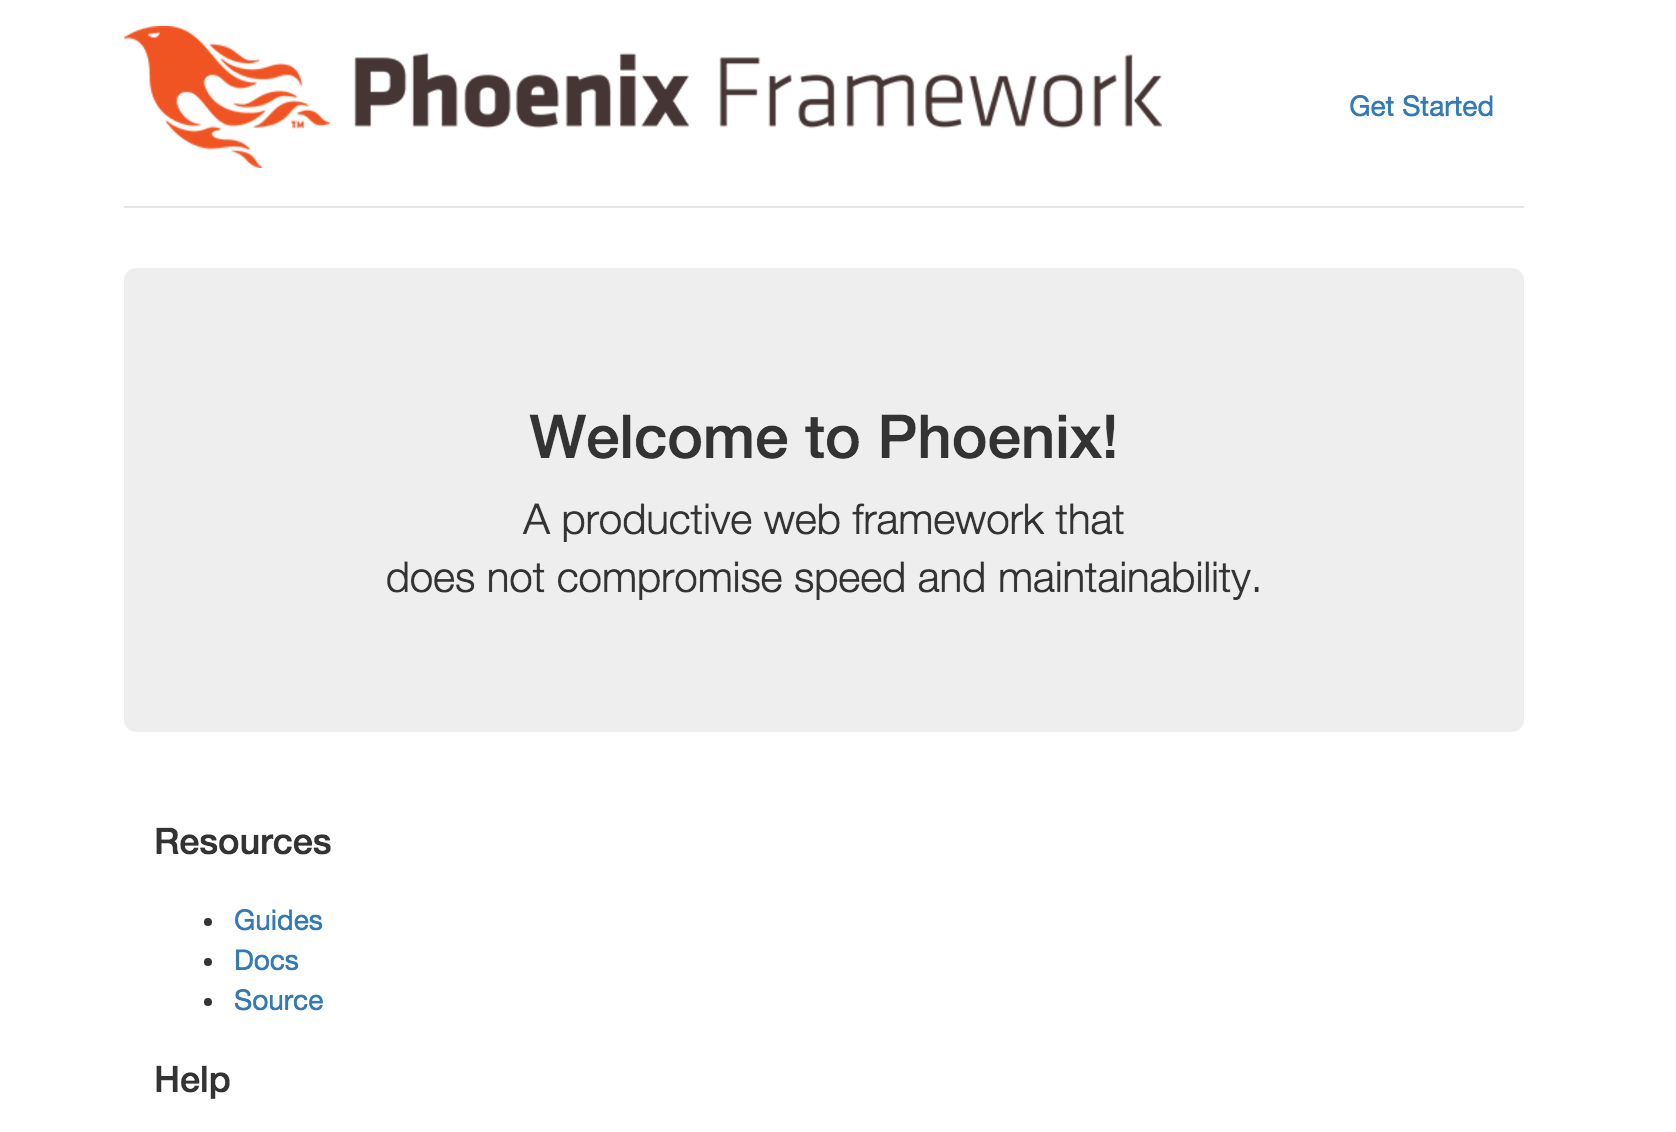
\includegraphics[width=1\linewidth]{Documentation/figures/phoenix_welcome_page.png}  % largura percentual
	\caption{Phoenix Front Page}
	\label{fig:phoenix}
\end{figure}

Looking at the body of the project, it has built-in generated folders and scripts:

\begin{itemize}
    \item a folder named "assets"
    \item a folder named "config"
    \item a folder named "lib"
    \item a folder named "priv"
    \item a folder named "test"
    \item dependancy files, such as "mix.exs", "mix.lock"
    \item README.md and .gitignore files
\end{itemize}

\begin{figure}[htbp]
	\centering
	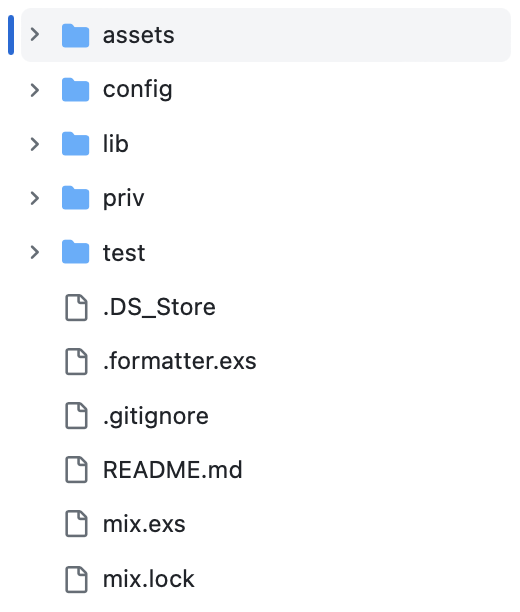
\includegraphics[scale=0.5]{Documentation/figures/phx-folders.png}  % largura percentual
	\caption{Phoenix Generated Files}
	\label{fig:phx}
\end{figure}

"Assets" folder contains the information responsible for the style of the application, like CSS and JavaScript files.

"Config" folder guards the necessary paths to connect the application, as well as signing salt and other cryptography information.

"Priv" folder contains the seeds file, migrations and static characteristics, like images.

"Test" folder, as the name says, stores automatic and manual tests than run in order to guarantee the safety and maintainability of the application.

"Lib" folder is probably the most important one of them all, since it stores two folders: \texttt{fake\_twitter} and \texttt{fake\_twitter\_web}. Each one of these folders has an \texttt{.ex} file related to it, which is the entrypoint for defining the application, such as web controllers, views, channels and everything that's necessary.

\begin{figure}[htbp]
	\centering
	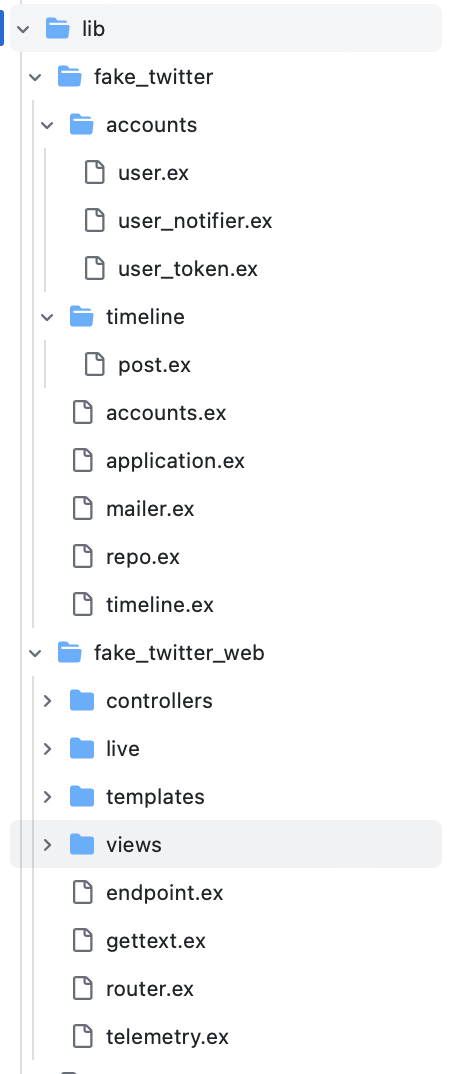
\includegraphics[scale=0.5]{Documentation/figures/lib.png}  % largura percentual
	\caption{Lib folder}
	\label{fig:phx}
\end{figure}

As it's clear to say, code organization plays a big role in Phoenix, since its folder structure is well divided and pristine. 

The directory \texttt{fake\_twitter} holds the core logic of the application. It includes modules responsible for business logic, data manipulation and domain-specific functionality. The project-specific code resides within this directory, and developers can organize it into subdirectories based on their application's structure.


However, inside \texttt{fake\_twitter\_web} directory, it focuses on the web-specific aspects of the Phoenix application. It contains:

\begin{itemize}
    \item \textit{Controllers}: This directory contains the controllers responsible for handling incoming requests, processing data and generating responses. Controllers are modules that define actions corresponding to different routes, implementing the application's business logic.
    \item \textit{Views}: The \texttt{views} directory holds the modules responsible for rendering templates and generating responses. Views provide a separation of concerns by handling the presentation layer, allowing developers to focus on generating the appropriate response format (e.g., HTML, JSON).
    \item \textit{Templates}: This directory stores the \textit{EEx} templates used by the views. \textit{EEx} is Phoenix's embedded Elixir templating engine, enabling dynamic content generation within HTML, XML or other response formats.
    \item \textit{Static Assets}: The \texttt{static} directory contains static assets such as JavaScript, CSS, images and other files used by the client-side of the application.
    \item \textit{router.ex}: The \texttt{router.ex} file defines the routing configuration for the application. It maps incoming HTTP requests to the appropriate controller actions using a declarative DSL (Domain-Specific Language) provided by Phoenix.
    \item Other files and folders necessary for the correct architecture of the application, such as helpers, error handlers and more.
\end{itemize}

Of course, the user can choose whether they want to add or delete some files/folders. For instance, Phoenix's default database is the relational database PostgreSQL. The user, however, can choose not to create a database or to use another one. But, for its practicality, the default database was used during this project.\newline

The project's features are shown in the figures:

\begin{figure}[htbp]
	\centering
	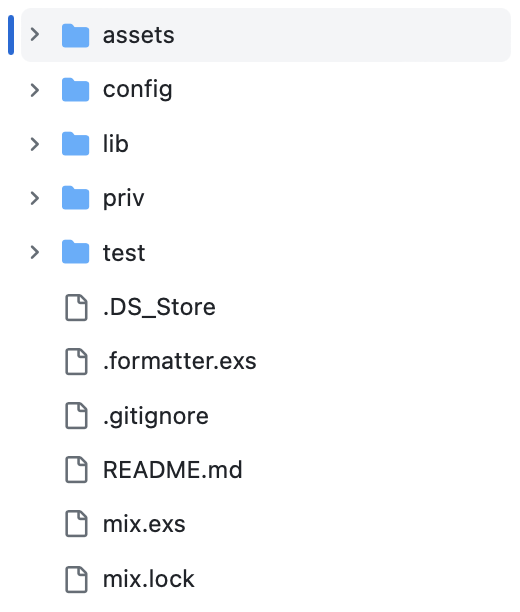
\includegraphics[scale=0.5]{Documentation/figures/phx-folders.png}  % largura percentual
	\caption{Phoenix Generated Files}
	\label{fig:phx}
\end{figure}



\begin{figure}[htbp]
	\centering
	
	\begin{minipage}[b]{0.45\textwidth}
		\centering
		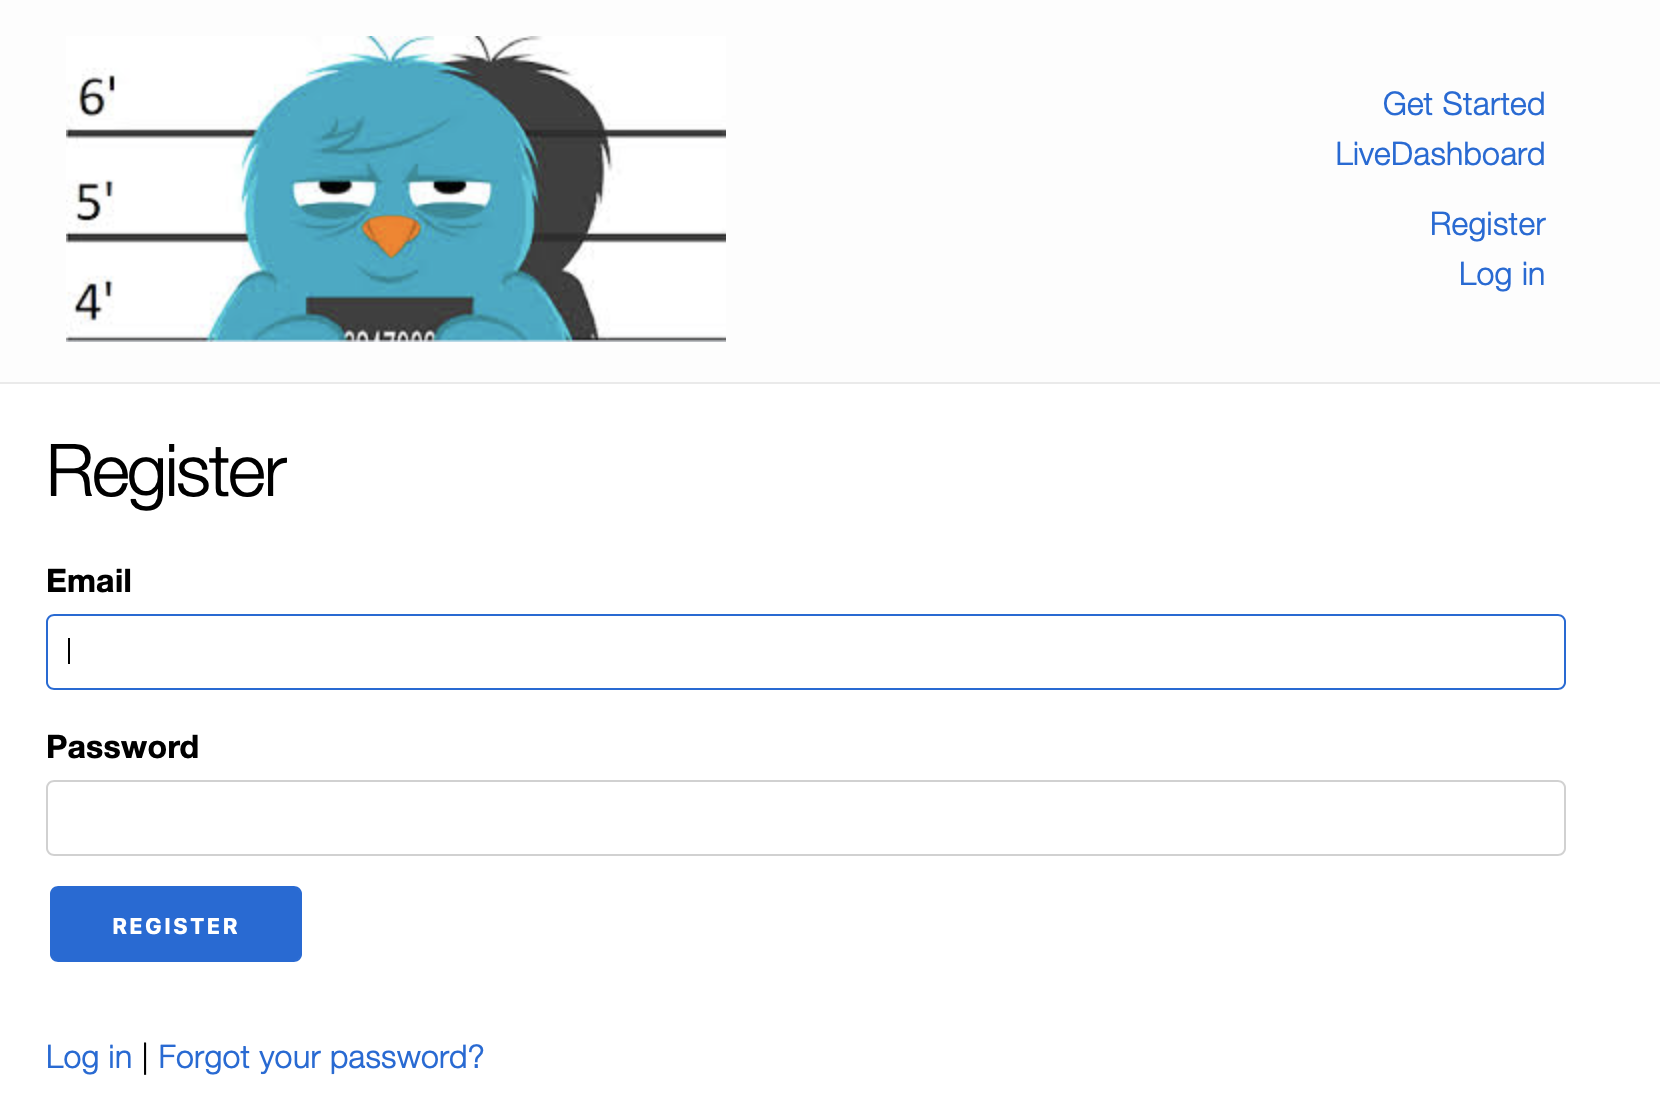
\includegraphics[width=\linewidth]{Documentation/figures/FT_register.png}
		\caption{Register User}
		\label{fig:register}
	\end{minipage}
	\hfill
	\begin{minipage}[b]{0.45\textwidth}
		\centering
		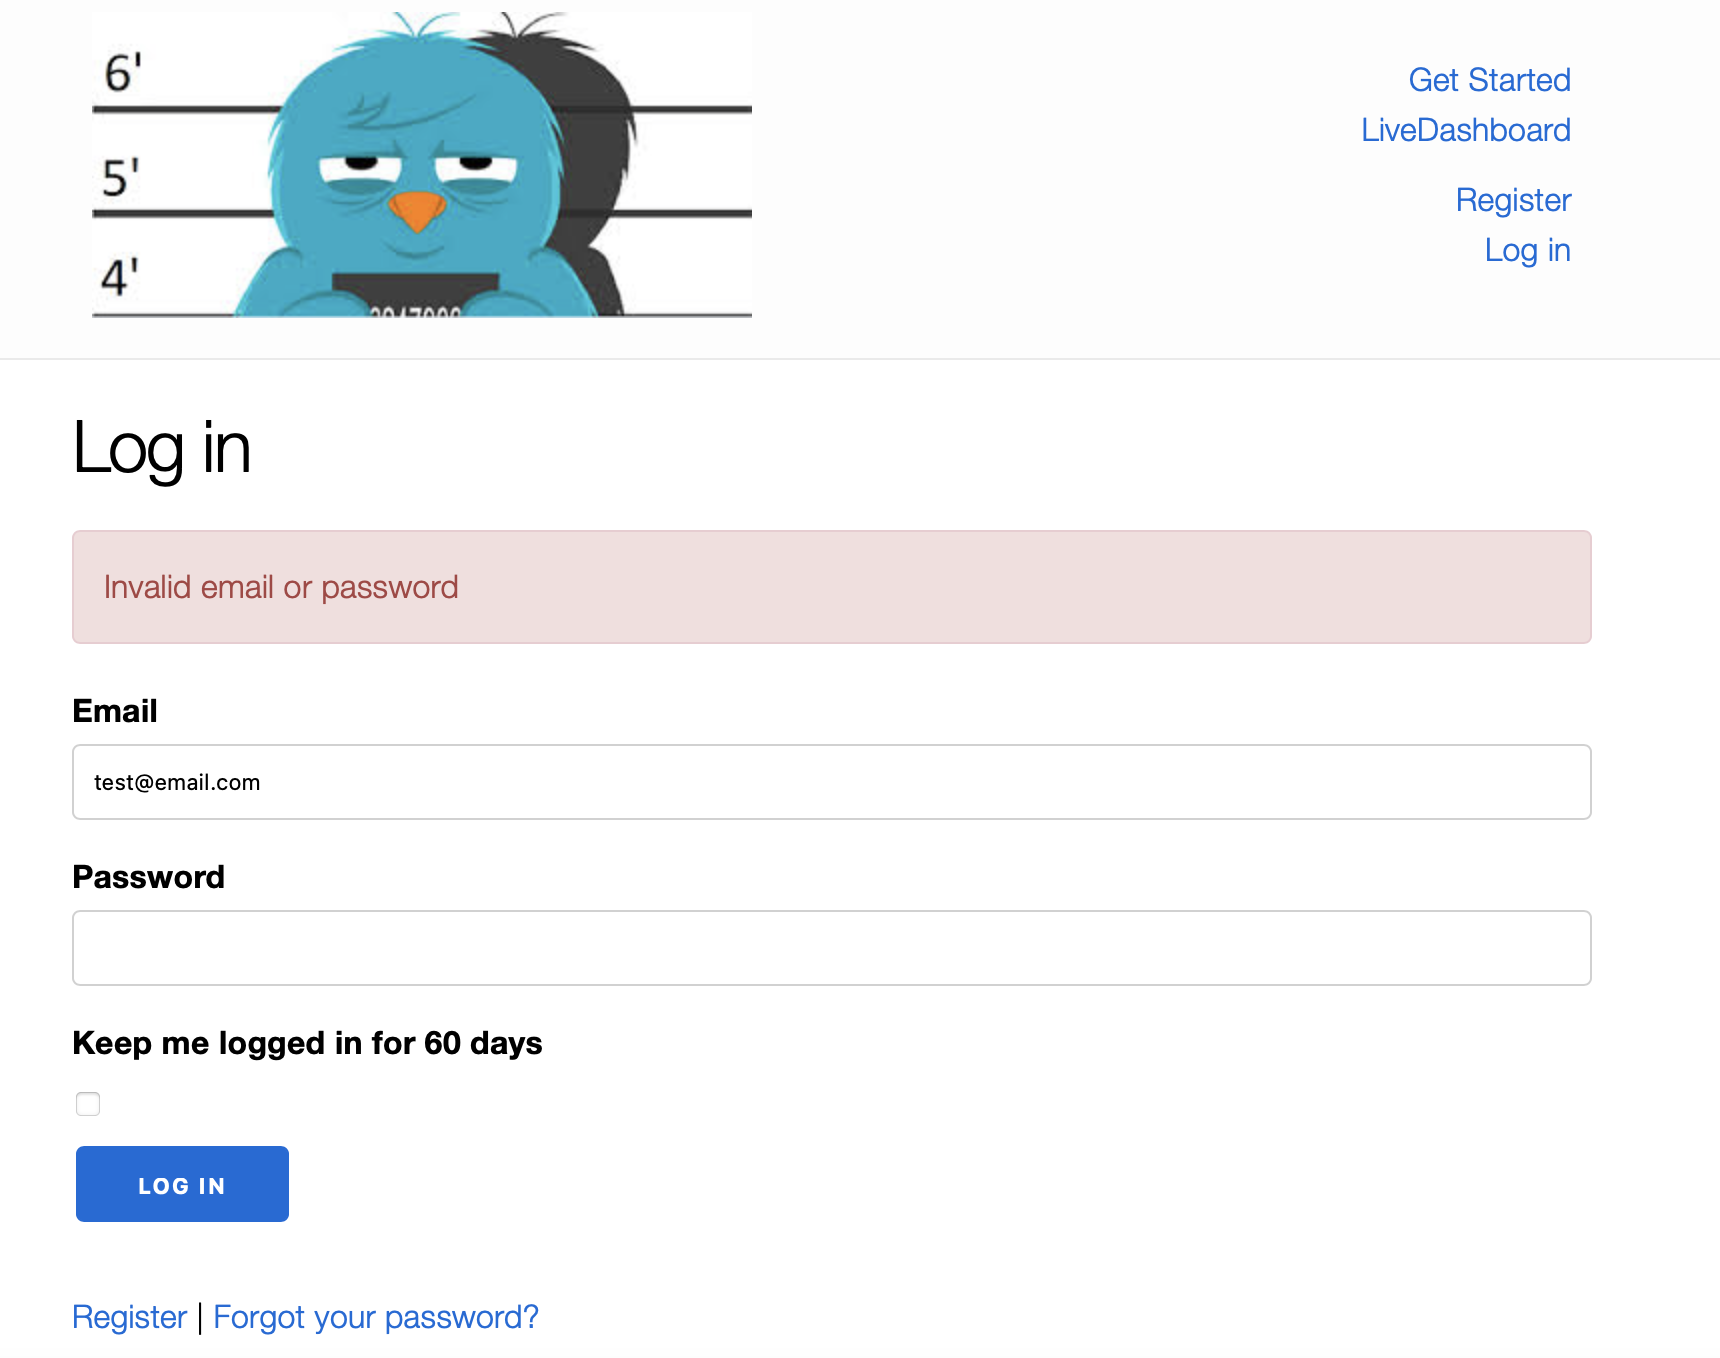
\includegraphics[width=\linewidth]{Documentation/figures/inv_email.png}
		\caption{Invalid Email}
		\label{fig:inv}
	\end{minipage}

\end{figure}

\begin{figure}[htbp]
	\centering
	
	\begin{minipage}[b]{0.45\textwidth}
		\centering
		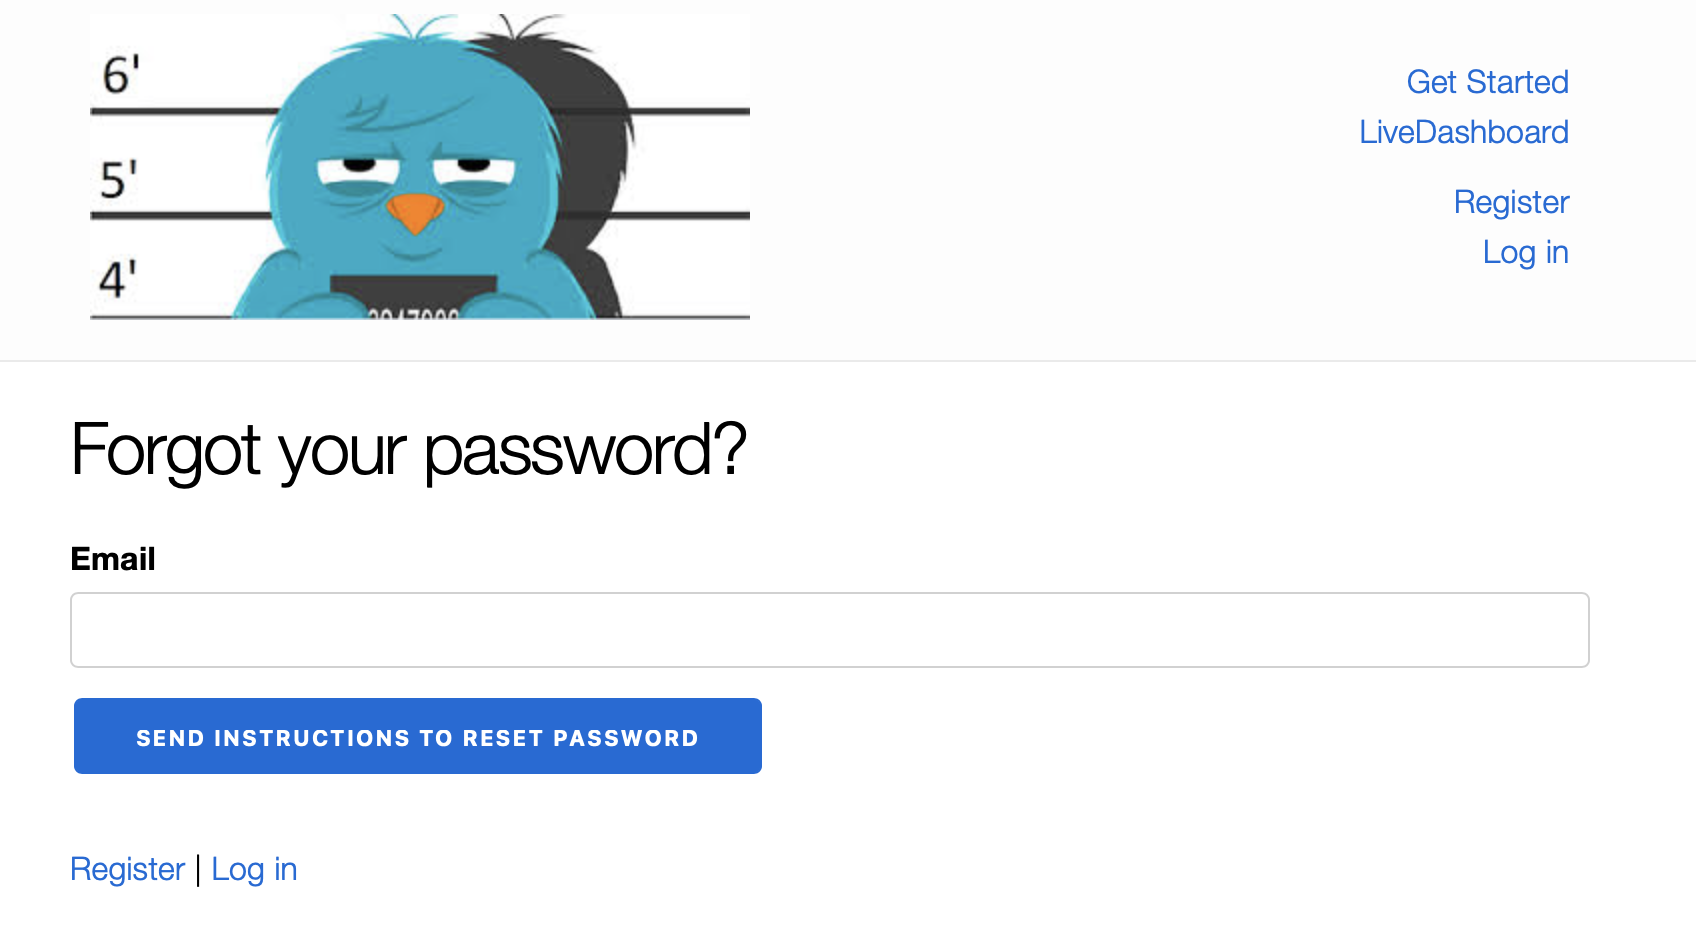
\includegraphics[width=\linewidth]{Documentation/figures/FT_forgot_pw.png}
		\caption{Forgot Password}
		\label{fig:pw}
	\end{minipage}
	\hfill
	\begin{minipage}[b]{0.45\textwidth}
		\centering
		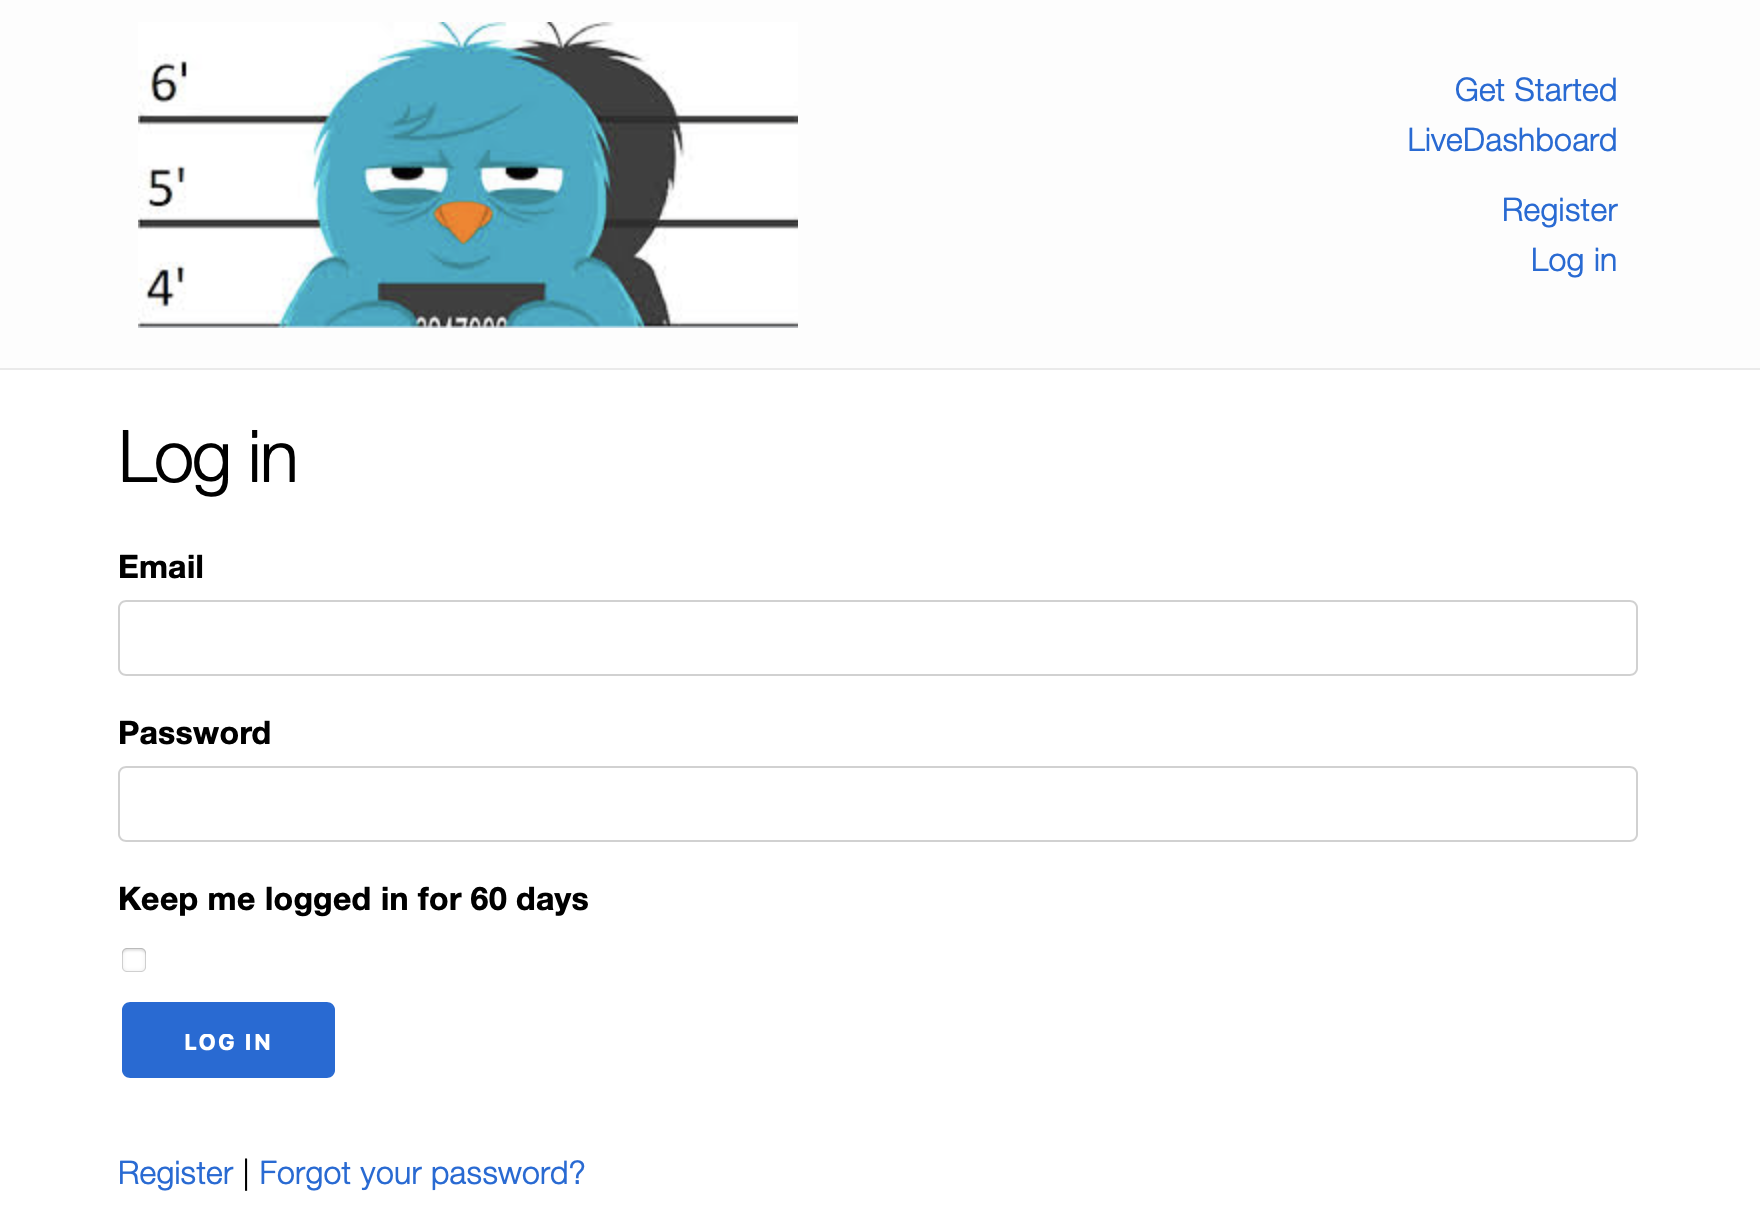
\includegraphics[width=\linewidth]{Documentation/figures/FT_login.png}
		\caption{Login}
		\label{fig:login}
	\end{minipage}

\end{figure}

\begin{figure}[htbp]
	\centering
	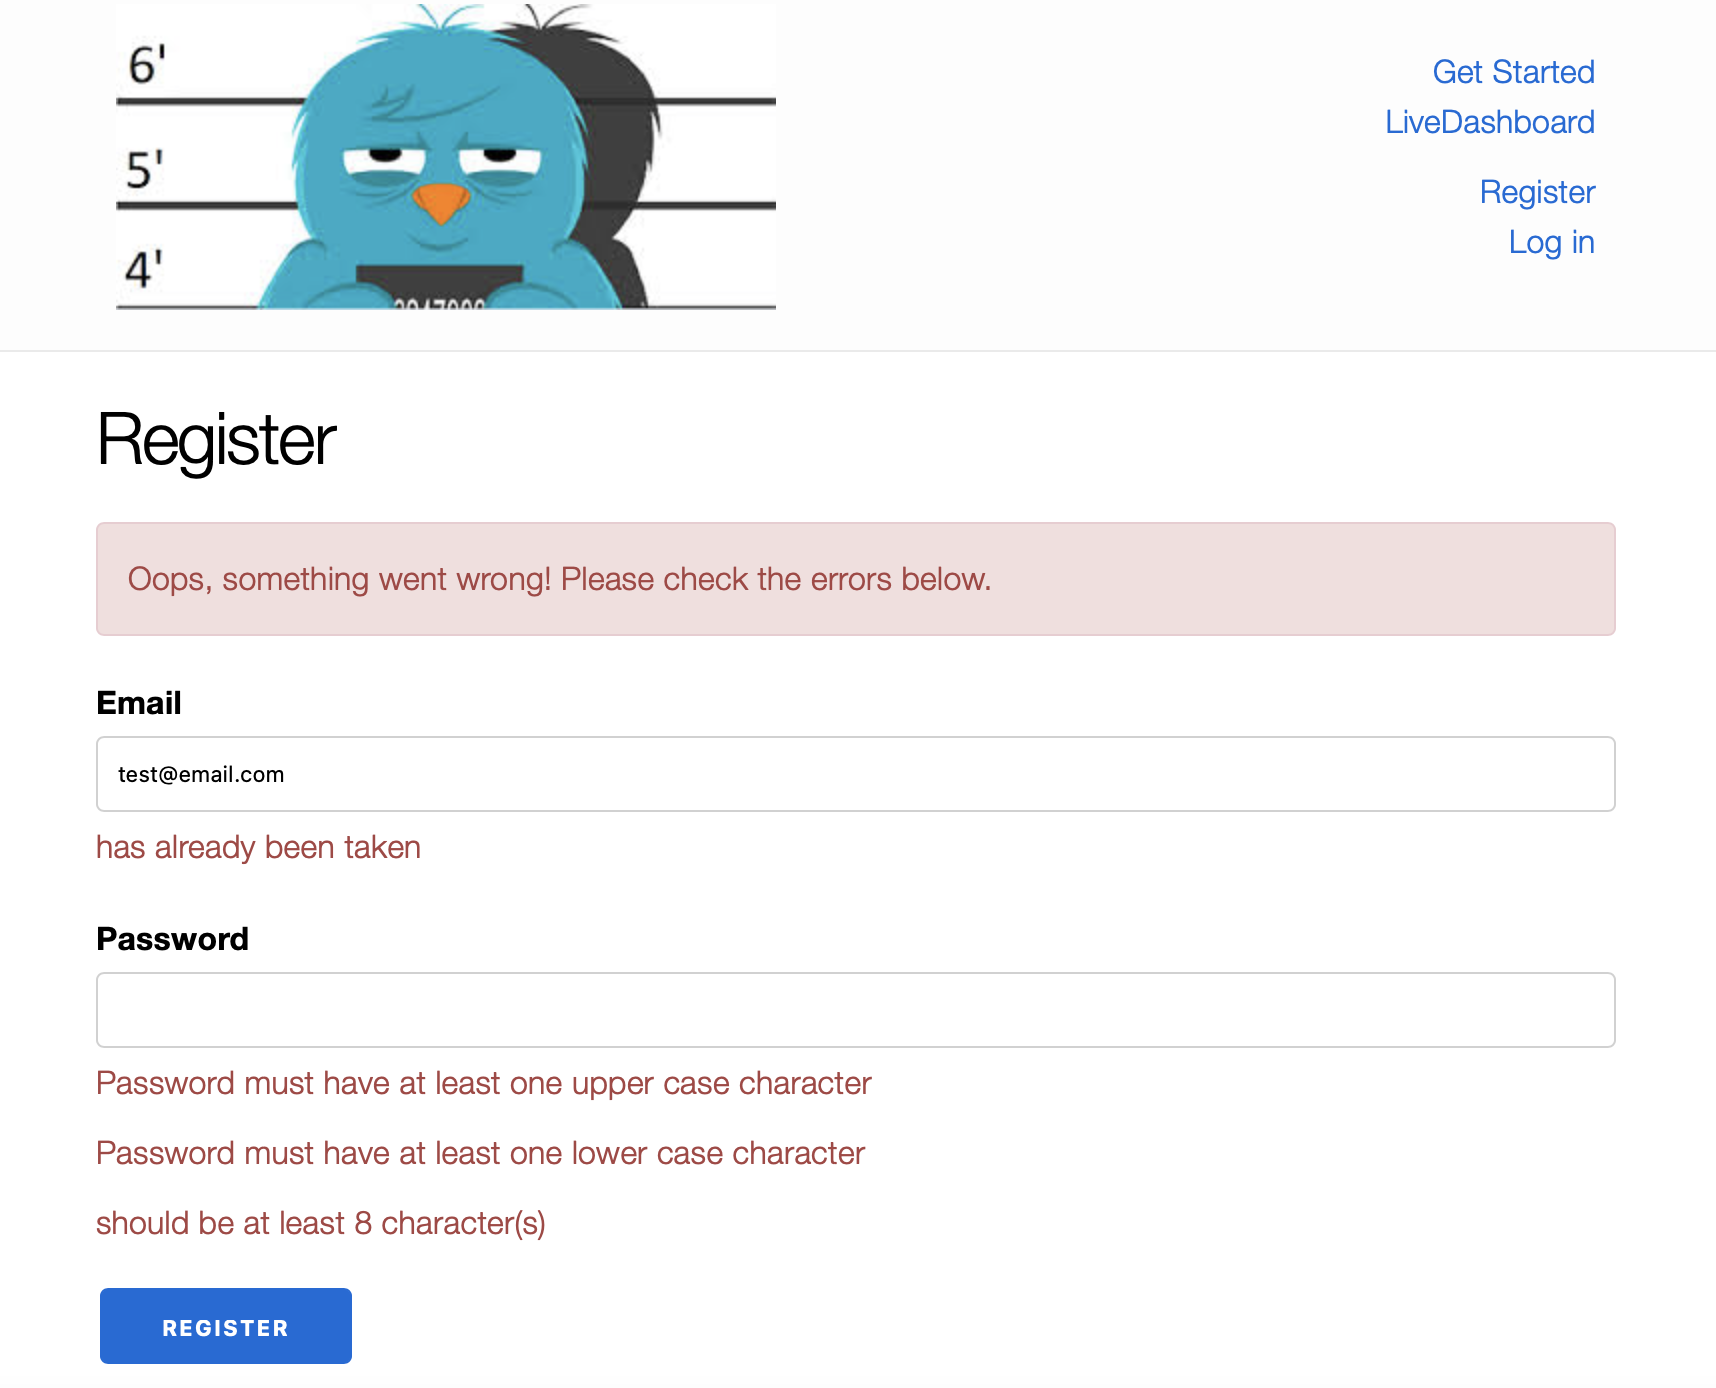
\includegraphics[scale=0.25]{Documentation/figures/sec.png}  % largura percentual
	\caption{Security features when creating an account}
	\label{fig:sec}
\end{figure}


\begin{figure}[htbp]
	\centering
	
	\begin{minipage}[b]{0.45\textwidth}
		\centering
		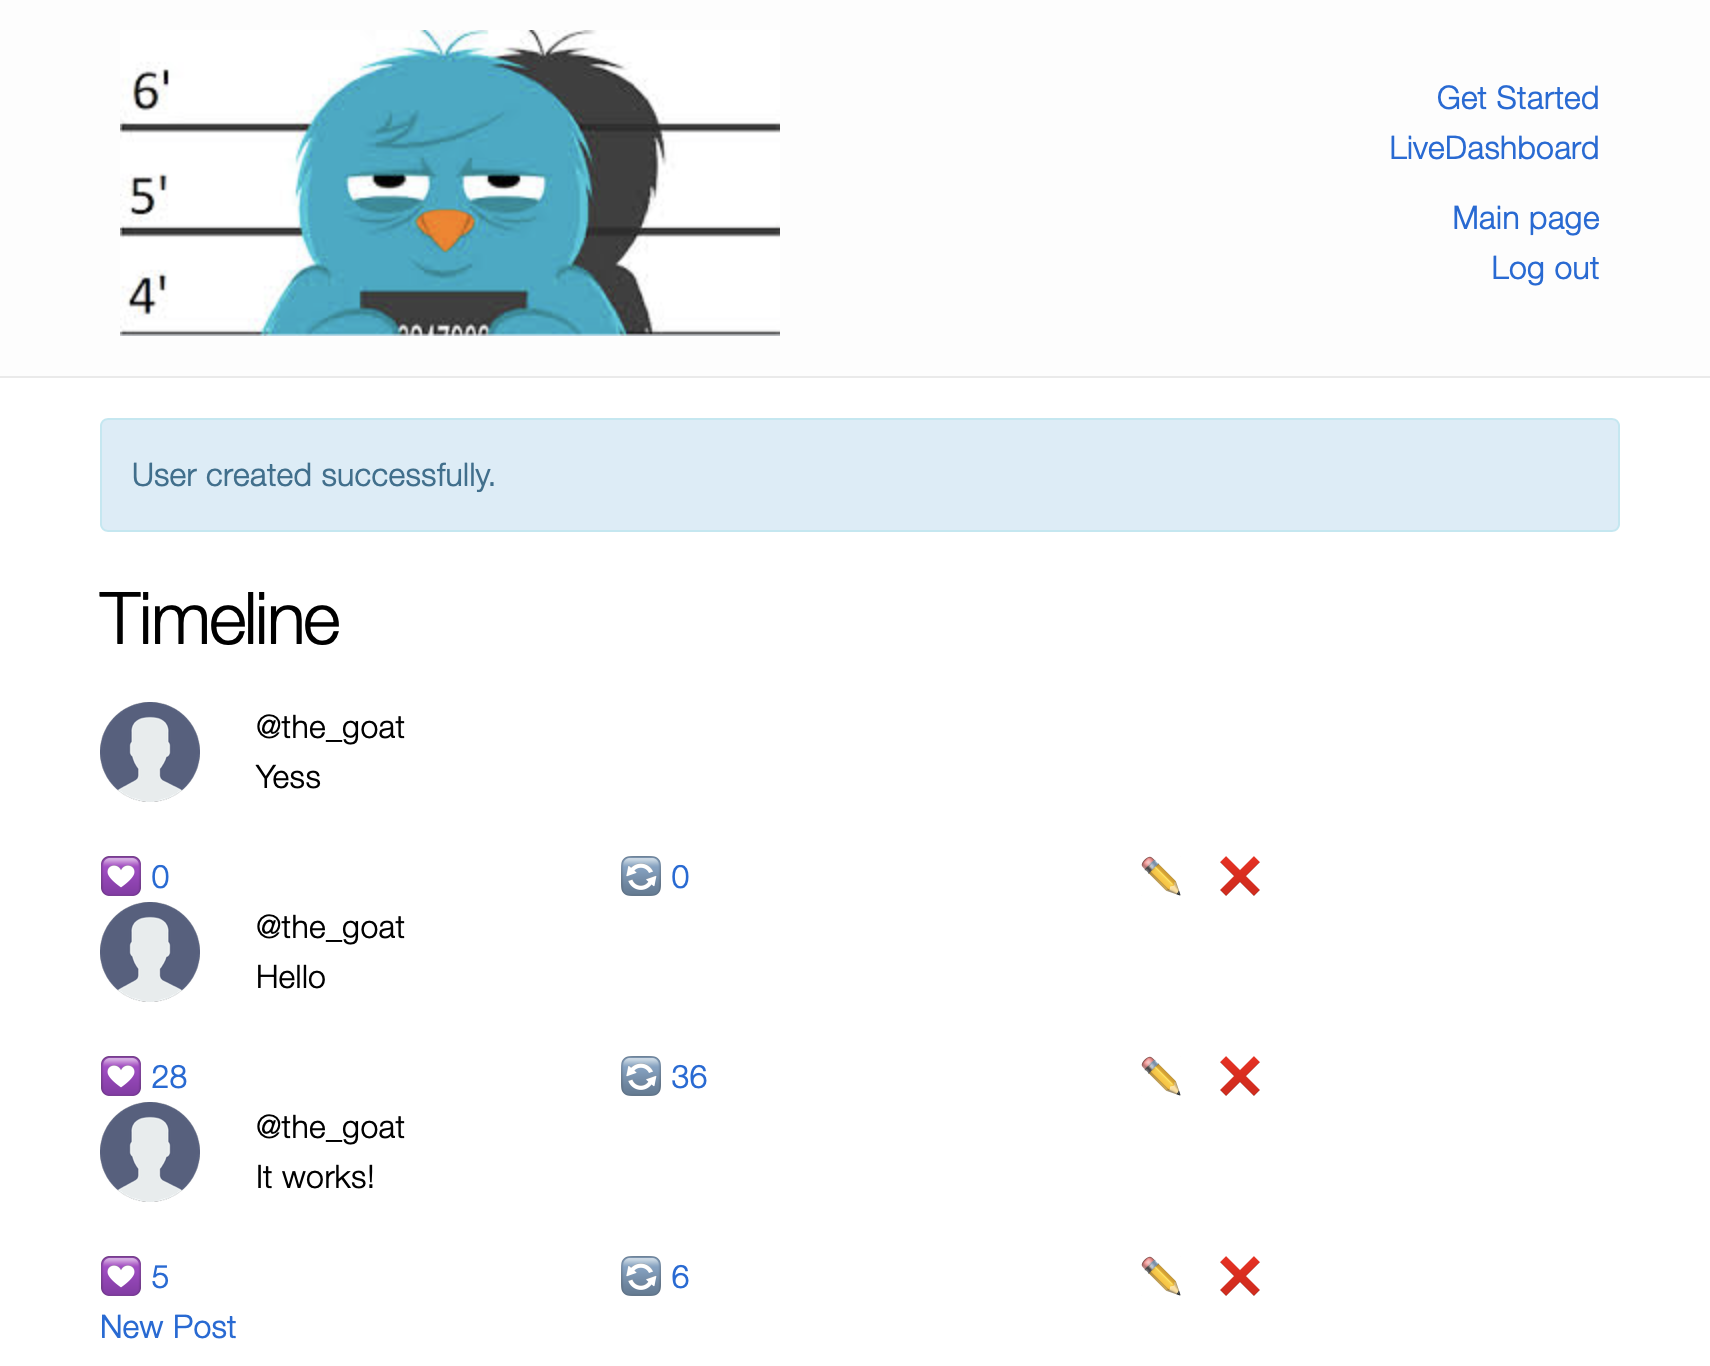
\includegraphics[width=\linewidth]{Documentation/figures/created_user.png}
		\caption{New user created}
		\label{fig:user}
	\end{minipage}
	\hfill
	\begin{minipage}[b]{0.45\textwidth}
		\centering
		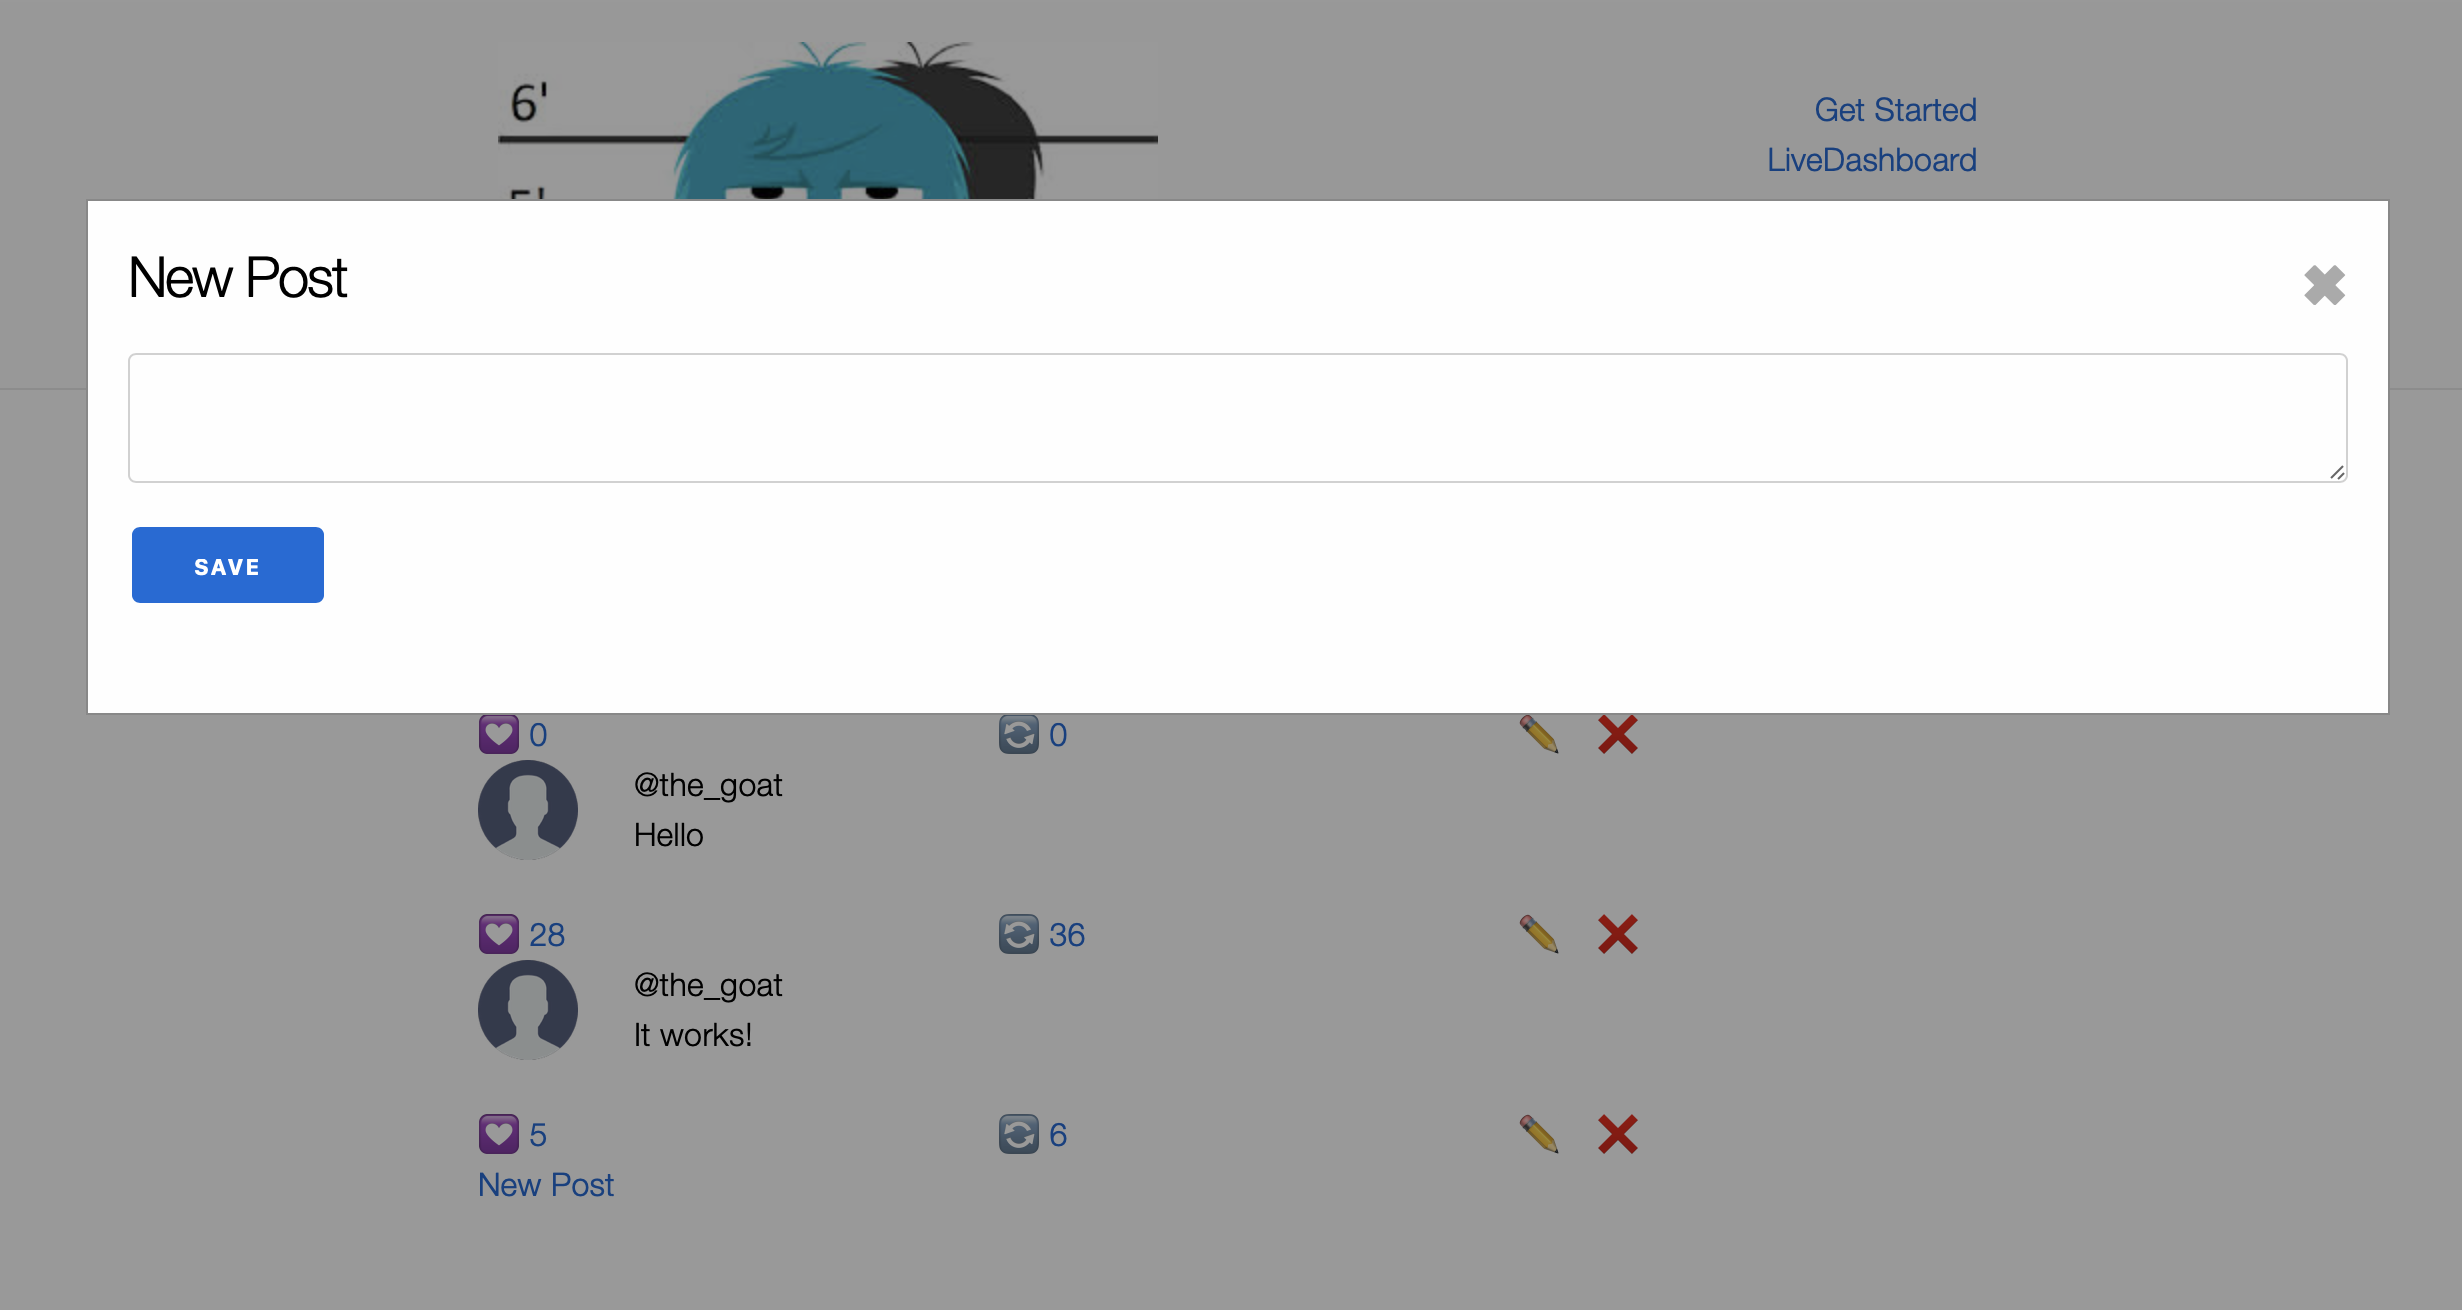
\includegraphics[width=\linewidth]{Documentation/figures/new_post.png}
		\caption{Create new post}
		\label{fig:np}
	\end{minipage}

\end{figure}


\begin{figure}[htbp]
	\centering
	
	\begin{minipage}[b]{0.45\textwidth}
		\centering
		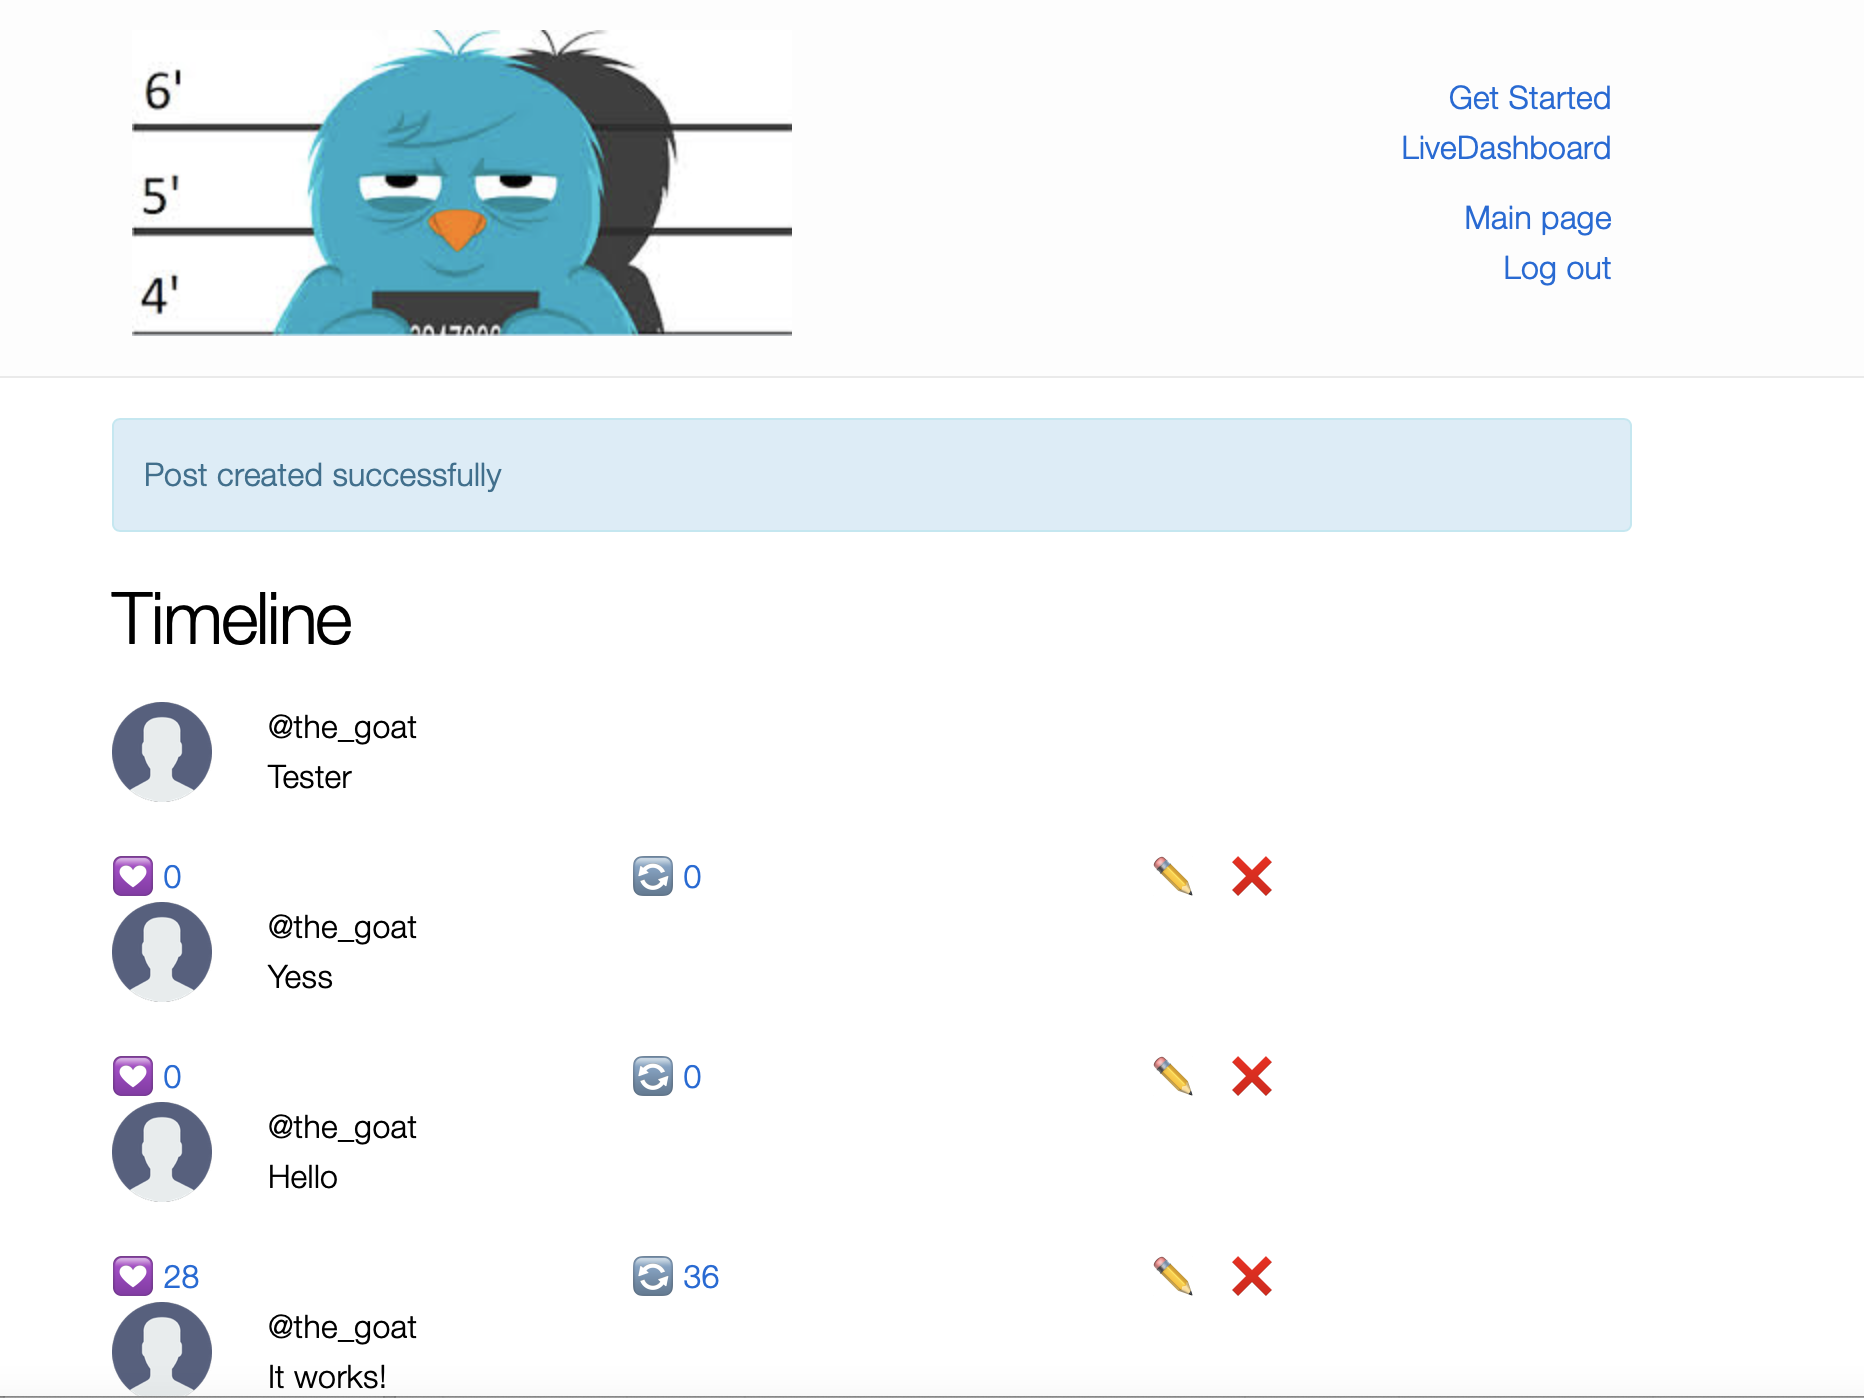
\includegraphics[width=\linewidth]{Documentation/figures/post.png}
		\caption{Post}
		\label{fig:post}
	\end{minipage}
	\hfill
	\begin{minipage}[b]{0.45\textwidth}
		\centering
		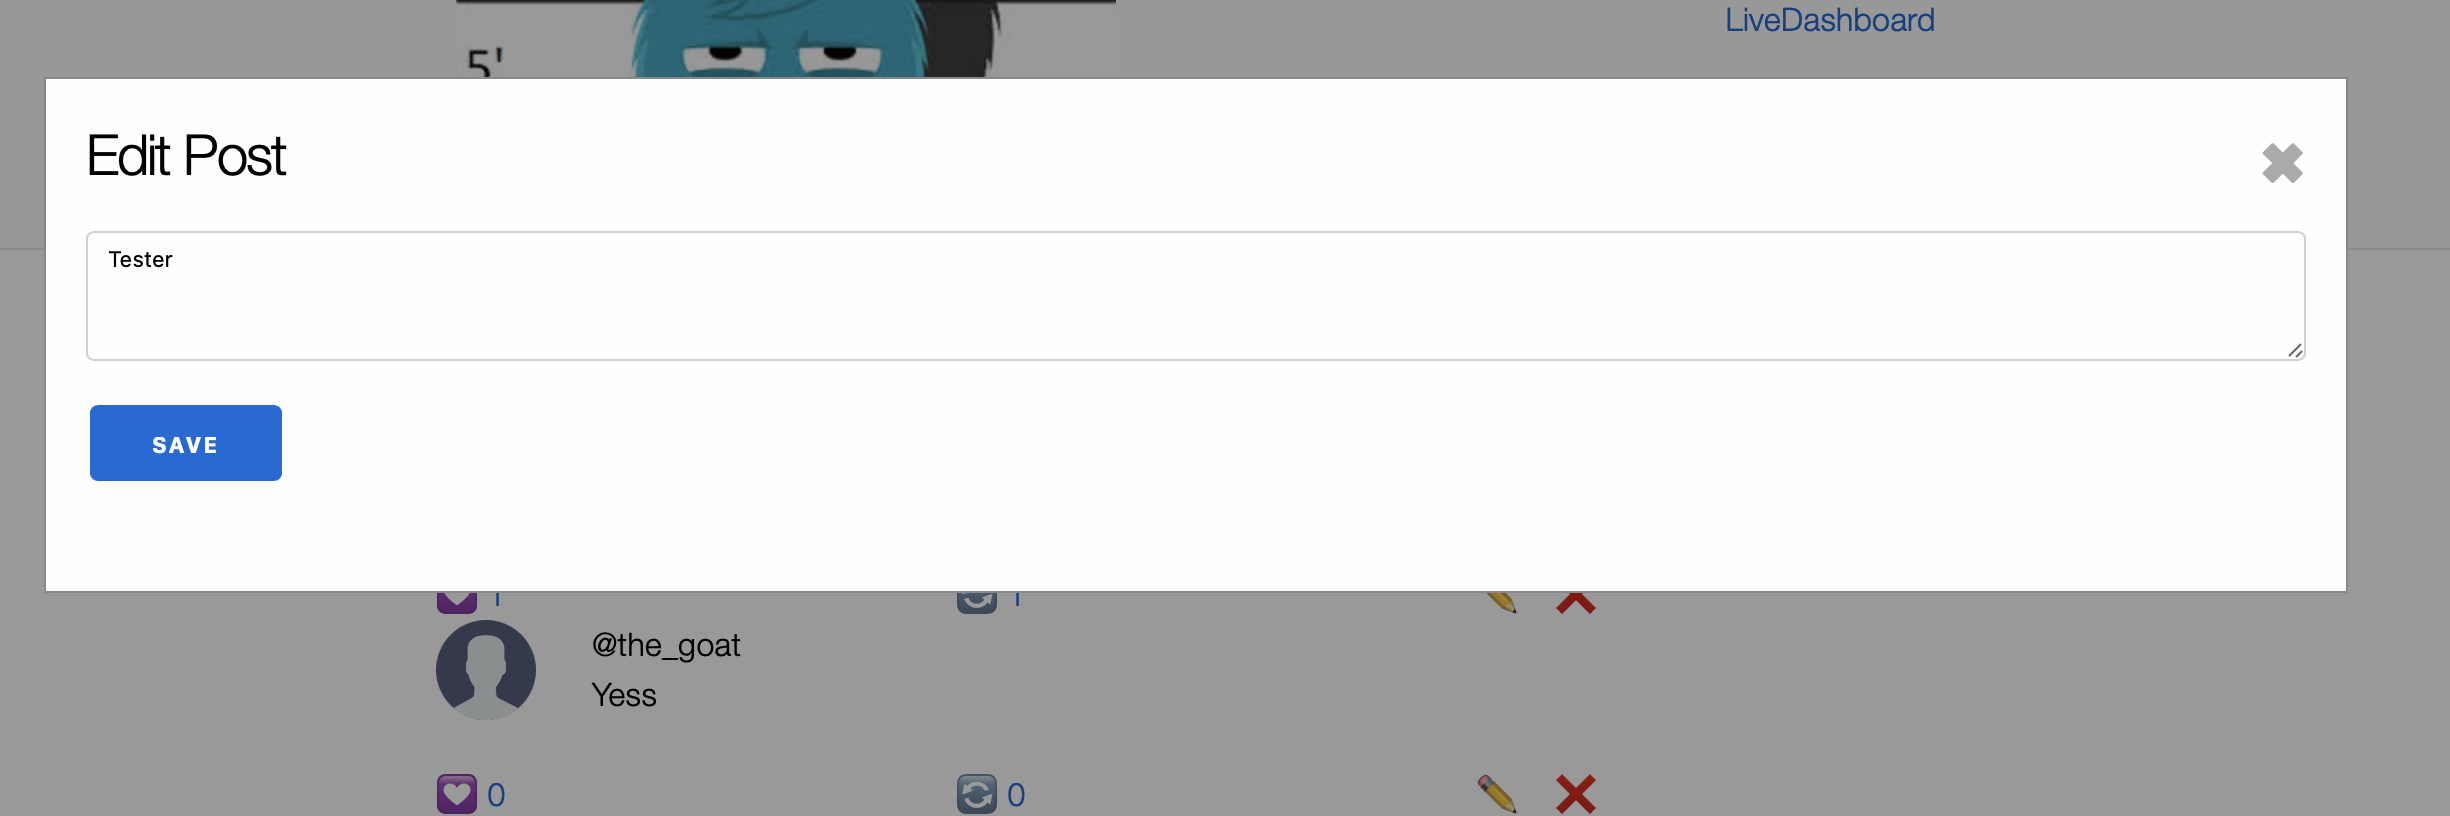
\includegraphics[width=\linewidth]{Documentation/figures/edit.png}
		\caption{Edit post}
		\label{fig:edit}
	\end{minipage}

\end{figure}

\begin{figure}[htbp]
	\centering
	
	\begin{minipage}[b]{0.45\textwidth}
		\centering
		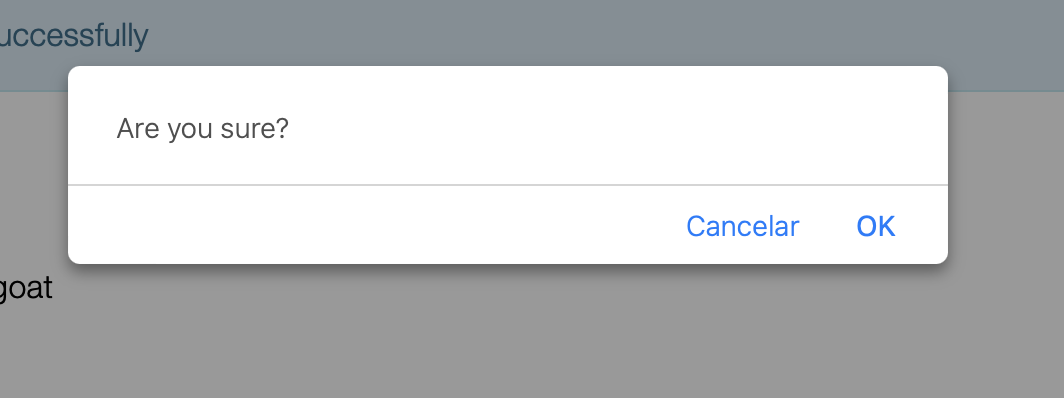
\includegraphics[width=\linewidth]{Documentation/figures/delete.png}
		\caption{Delete post notification}
		\label{fig:delete}
	\end{minipage}
	\hfill
	\begin{minipage}[b]{0.45\textwidth}
		\centering
		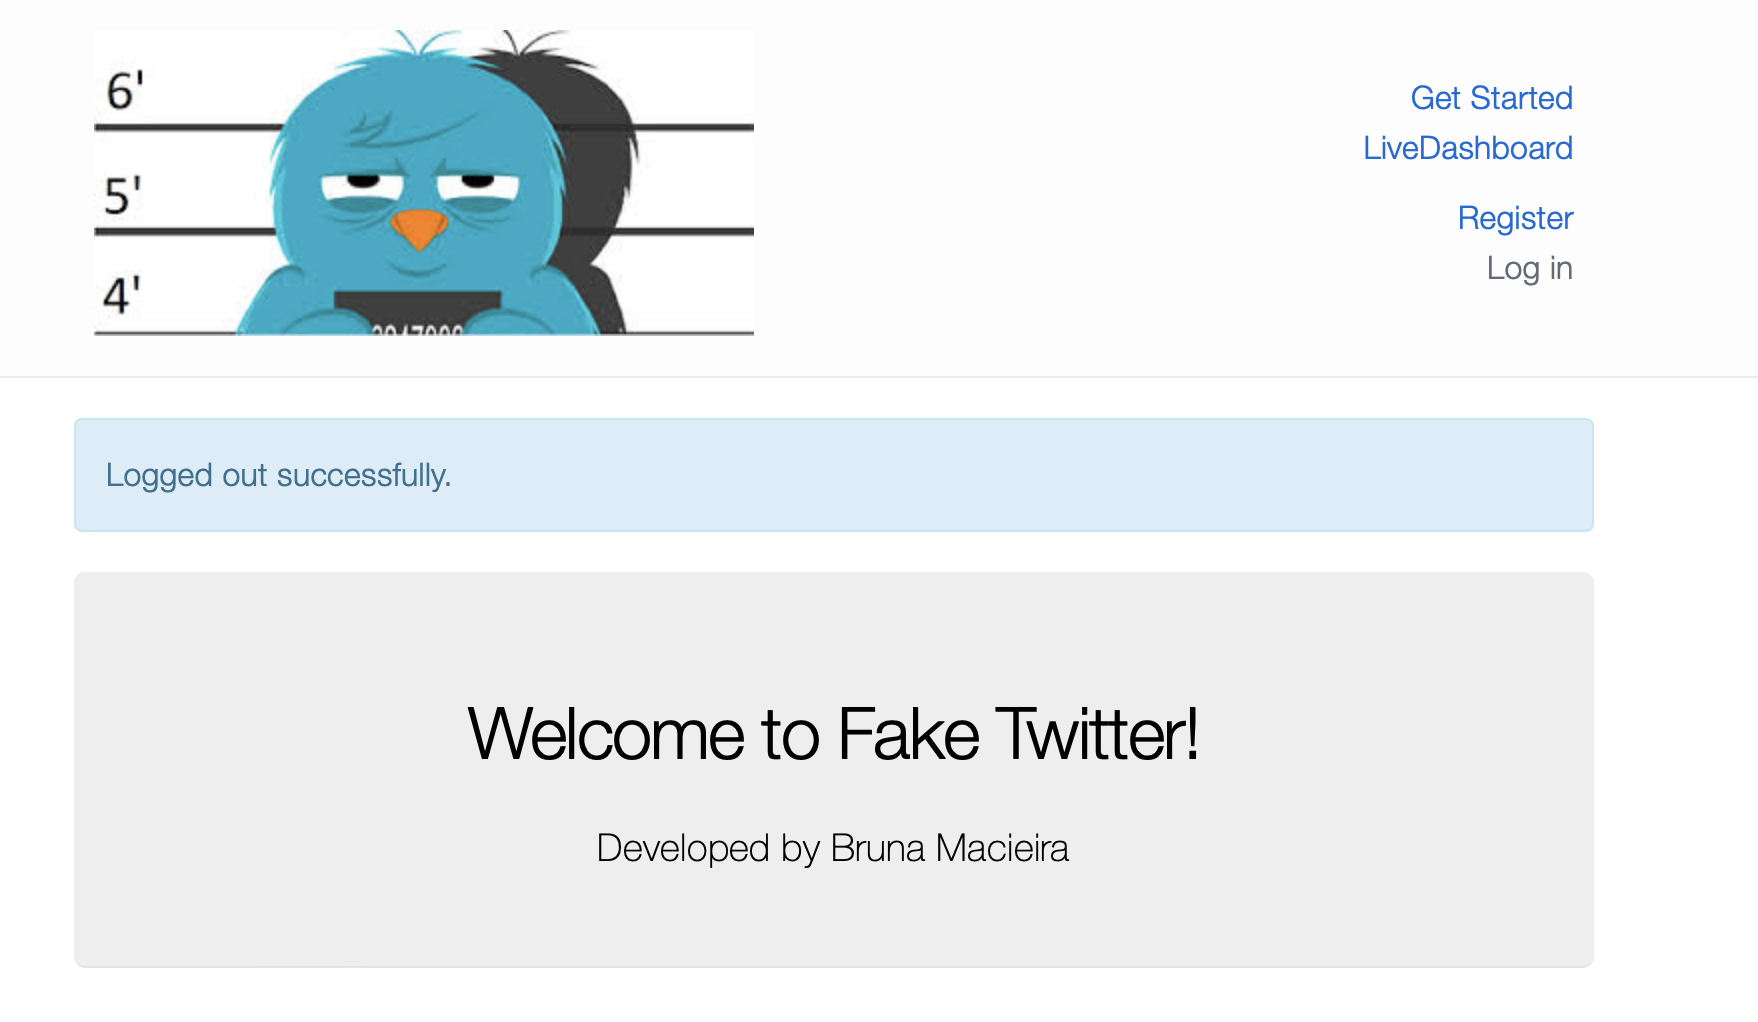
\includegraphics[width=\linewidth]{Documentation/figures/logout.png}
		\caption{Logout}
		\label{fig:logout}
	\end{minipage}

\end{figure}



Users' information, like posts, email and so on, can be checked on tools like PG-Admin (see section \ref{post}). Regarding a tip given by a Yarilabs employee, \href{https://eggerapps.at/postico2/}{\textit{Postico}}\footnote{For a further understanding of Postico, please check: https://eggerapps.at/postico2/} was used.

\begin{figure}[htbp]
	\centering
	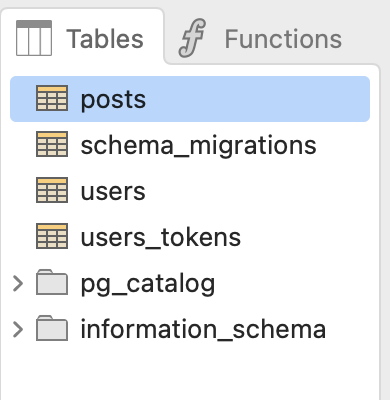
\includegraphics[scale=0.5]{Documentation/figures/postico.png}  % largura percentual
	\caption{Postico's data}
	\label{fig:postico}
\end{figure}


\section{Tentacat} \label{tentacat}

\textit{Tentacat} is a \textit{GitHub wrapper} for Elixir. It allows Elixir developers to seamlessly integrate their applications with GitHub's extensive functionality and data.

With Tentacat, various operations can be performed on GitHub repositories, issues, pull requests, organizations, users, and more. It simplifies the process of authenticating with the GitHub API, making requests, and handling responses, providing a convenient interface for building GitHub-related functionality into Elixir applications.

Tentacat leverages the power of Elixir's concurrency model and functional programming paradigm to offer efficient and reliable interactions with the GitHub API. It provides a set of expressive and intuitive functions to query and manipulate GitHub resources, making it easier to retrieve information, create or update repositories, manage issues, and perform other GitHub-related tasks programmatically.

Some key features and benefits of Tentacat include:

\begin{itemize}
    \item \textit{GitHub API Integration}: Tentacat seamlessly integrates with the GitHub API, allowing developers to interact with GitHub's vast ecosystem of features and data.
    \item \textit{Authentication}: Tentacat provides authentication mechanisms, including personal access tokens and OAuth, to securely access the GitHub API on behalf of users or applications.
    \item \textit{Resource Operations}: Tentacat offers a rich set of functions to perform operations on GitHub resources. Developers can create, read, update, and delete repositories, manage issues and pull requests, work with organizations and users, and more.
    \item \textit{Error Handling}: Tentacat handles API errors and provides meaningful error messages and exceptions, making it easier to handle and recover from potential issues.
    \item \textit{Concurrent Requests}: Built on top of Elixir's concurrency model, Tentacat allows developers to make concurrent requests to the GitHub API, improving performance and responsiveness of applications.
    \item \textit{Extensibility}: Tentacat is designed to be extensible, allowing customization and extend its functionality as per the application's requirements.
    \cite{tentacat}
\end{itemize}

Tentacat can be a valuable asset in Elixir development toolkit and it sure was when it came to Dharma Network.

\begin{figure}[htbp]
	\centering
	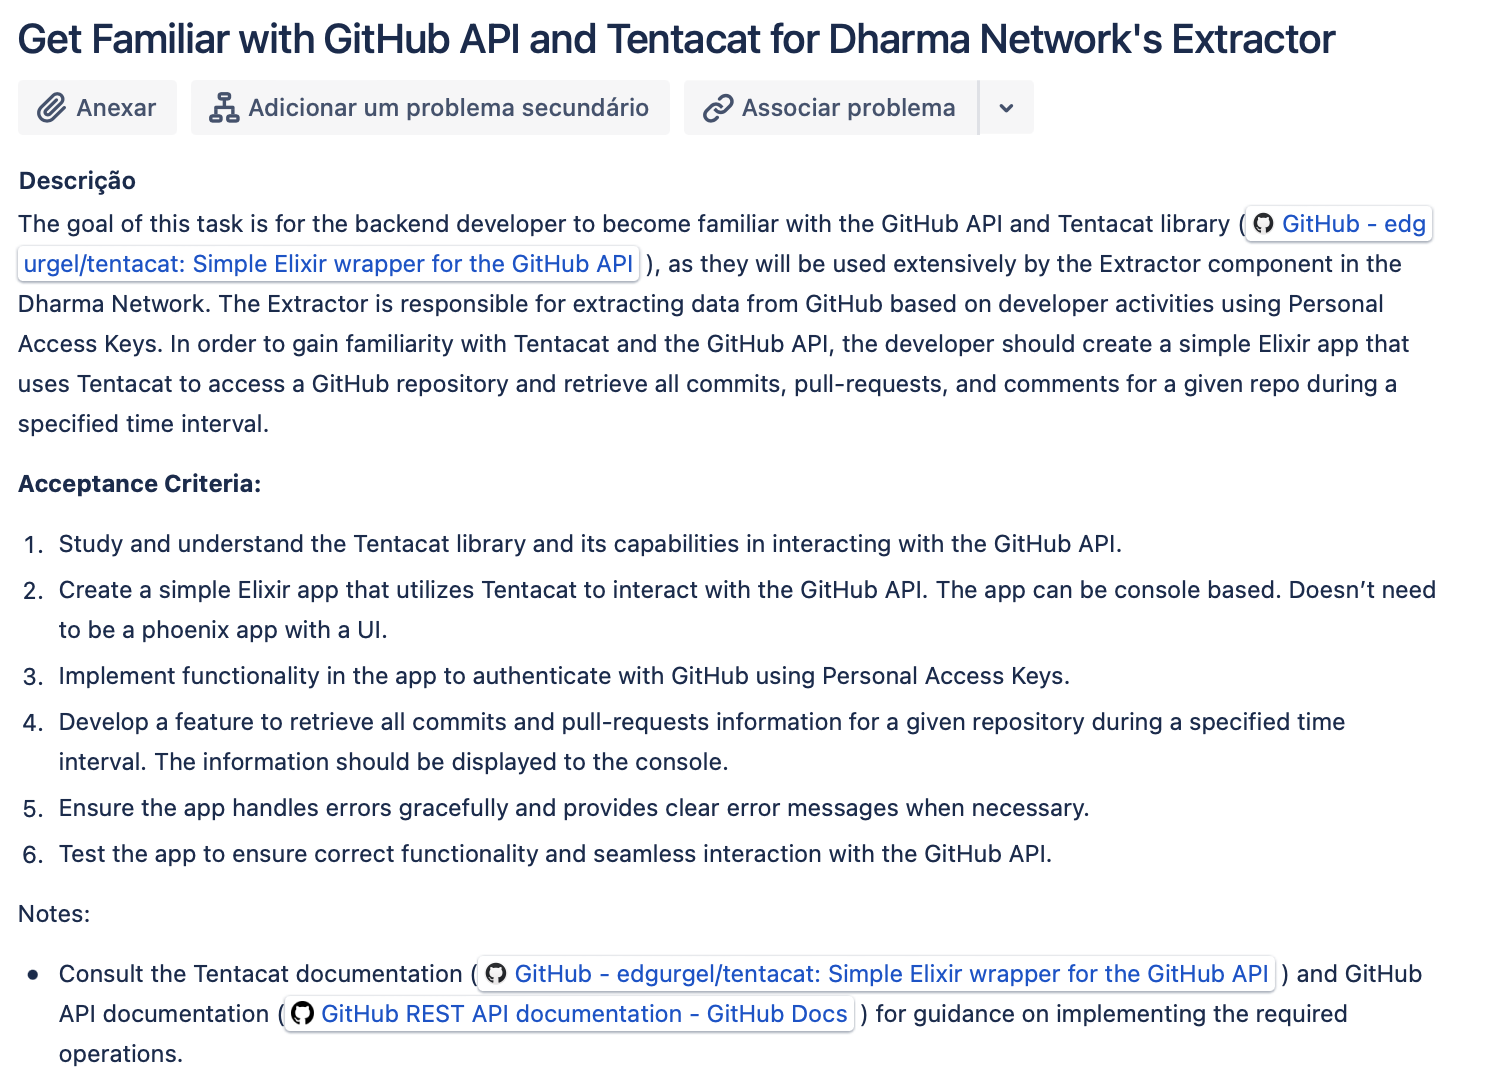
\includegraphics[scale=0.5]{Documentation/figures/ticket.png}  % largura percentual
	\caption{Tentacat's ticket}
	\label{fig:ticket}
\end{figure}

As seen on the figure \ref{fig:ticket}, it was up for the developer to become familiar with GitHub API (see \ref{github}), since it's a key resource to be consumed by Dharma Network.

This component, in similarity to the previous study objects, took a vast learning period, as it was of extreme importance.\newline

Since there's not a lot of resources online about this tool, the available ones were scrupulously analyzed. The main resources were the \href{https://github.com/edgurgel/tentacat}{\textit{Tentacat source code}}\footnote{To check Tentacat's source code, please check: https://github.com/edgurgel/tentacat} and \href{https://hexdocs.pm/tentacat/readme.html}{\textit{Tentacat Hex files}}\footnote{To check Tentacat's Hex files, please check: https://hexdocs.pm/tentacat/readme.html}. \newline

Once the basics of Tentacat and GitHub API were understood, a project named \texttt{tentahub} (Tentacat + GitHub) was created.

\begin{figure}[htbp]
	\centering
	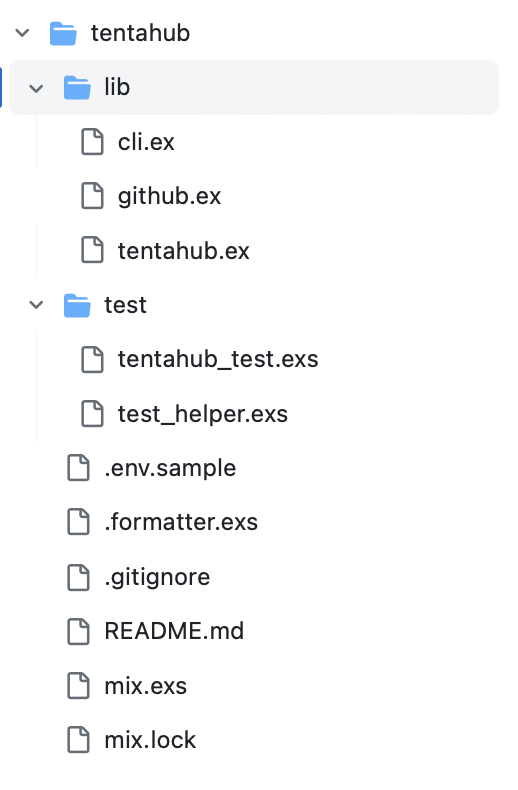
\includegraphics[scale=0.5]{Documentation/figures/tentahub.png}  % largura percentual
	\caption{Tentacat's files}
	\label{fig:tent}
\end{figure}

As seen on image \ref{fig:tent}, the project's main folder is called \texttt{lib}. This folder contains 3 files, responsible for: connecting to the GitHub API, extracting the data and running the application. Also, the file \texttt{env.sample} contains then necessary user information to fetch the GitHub data, which is confidential, and is why, before running the program, the command {
\newcommand{\shellcmd}[1]{\\\indent\indent\texttt{\footnotesize\# #1}\\}
  \shellcmd{cp .env.sample .env}
}should be ran, in order to create an editable file where confidential information can be stored.\newline

Then, the command {
\newcommand{\shellcmd}[1]{\\\indent\indent\texttt{\footnotesize\# #1}\\}
  \shellcmd{mix guardian.gen.secret}
} should be compiled in order to generate a JWT secret, necessary for the execution of the application.\newline

That information should be stored here, substituting the information between brackets:

\begin{lstlisting}[language=Erlang, caption={.env.sample}]
export GITHUB_TOKEN=<your-token>
export GITHUB_OWNER=<repository-owner>
export GITHUB_REPO=<repository-name>
export SINCE_DATE=<start-date>
export UNTIL_DATE=<end-date>
\end{lstlisting}

Analyzing the \texttt{tentahub} project, it's shown:

\begin{lstlisting}[language=Erlang, caption={github.ex}]
    defmodule GitHub do
  def get_commits(client, owner, repo, since, until) do
    filters = [since: since, until: until, per_page: 100]
    Tentacat.Commits.filter(client, owner, repo, filters)
  end

  def get_pull_requests(client, owner, repo, since, until) do
    filters = [state: "all", sort: "created", direction: "asc", since: since, until: until, per_page: 100]
    Tentacat.Pulls.filter(client, owner, repo, filters)
  end

  def get_comments(client, owner, repo, since, until) do
    Tentacat.Issues.Comments.list_all(client, owner, repo)
  end
end
\end{lstlisting} 

\begin{lstlisting}[language=Erlang, caption={tentahub.ex}]
    defmodule Tentahub do
  def run do
    Cli.run()
  end
end
\end{lstlisting}


\begin{lstlisting}[language=Erlang, caption={cli.ex}]
    defmodule Cli do
  def run do
    token = System.get_env("GITHUB_TOKEN")
    owner = System.get_env("GITHUB_OWNER")
    repo = System.get_env("GITHUB_REPO")
    since = System.get_env("SINCE_DATE")
    until = System.get_env("UNTIL_DATE")

    client = Tentacat.Client.new(%{access_token: token})

    commits = GitHub.get_commits(client, owner, repo, since, until)
    pull_requests = GitHub.get_pull_requests(client, owner, repo, since, until)
    comments = GitHub.get_comments(client, owner, repo, since, until)

    IO.puts "-----------------------Commits:------------------------------"
    IO.inspect commits

    IO.puts "-----------------------Pull requests:------------------------"
    IO.inspect pull_requests

    IO.puts "-----------------------Comments:-----------------------------"
    IO.inspect comments
  end
end
\end{lstlisting}

Although it might seem a simple application, the testing took awhile, since the correct information wasn't being retrieved.\newline

While doing this project, a better insight was uncovered regarding the structure of Github API. For instance, to retrieve specific information from pull requests \label{issue}, like to filter them by \texttt{since} date, the module \texttt{Pulls} is not enough; after some research, it was found that the module \texttt{Issues} was just right, since a pull request is always an issue, but an issue might not always be a pull request. Plus, it allows the filtering by \texttt{since} date.\newline

With the cessation of this project, we took a step closer to the main project.


\section{GitHub API} \label{github}

The GitHub API is a powerful application programming interface that allows developers to interact with the resources and data of the GitHub platform. As a leading platform for source code hosting and development collaboration, GitHub provides a rich set of APIs that enable developers to automate workflows, integrate with other tools, and build applications that leverage GitHub's functionality.\newline

With the GitHub API, developers can perform a wide range of operations, such as creating and managing repositories, accessing and manipulating issues and pull requests, retrieving user information, and much more. The API can programmatically interact with GitHub's features and integrate them into applications, tools, or scripts.\newline

The GitHub API follows the principles of REST (Representational State Transfer) and provides endpoints that return data in JSON format. It supports various authentication methods, including personal access tokens and OAuth, ensuring secure access to the API's capabilities.\newline

By leveraging the GitHub API, developers gain enhanced control and flexibility in managing their repositories, automating repetitive tasks, integrating with external services, and gaining insights into their development processes.\newline

When it comes to its usage in Dharma Network, it's a key resource, since the entire algorithm of the platform depends on it (as for the first release).\newline

As seen above (see section \ref{tentacat}), it was inserted onto the \texttt{tentahub} application, in order to collect data from a GitHub repository. 

The connection and filtering was accomplished by following the \href{https://docs.github.com/pt/rest/quickstart?apiVersion=2022-11-28}{\textbf{GitHub documentation}}\footnote{To check GitHub API's documentation, please check: https://docs.github.com/pt/rest/quickstart?apiVersion=2022-11-28}.

\section{Bug Hunting on Durga}\label{bug}

Following the training of such concepts, it was time to follow for the main project: Dharma Network. \newline
Dharma Network is divided into 3 categories: \textit{Rudra}, the web application frontend; \textit{Durga}, the backend services; and \textit{Algodex}, the Algorand SDK developed by Dharma Network. The exploited one in this section will be \textit{Durga}, the backend project.\newline

The first interaction with Durga was meant to understand its structure and components, which will be presented next chapter (see chapter \ref{chap:chap4}). \newline
One easy way to better understand the program and what it retrieves is by running the code. However, that was not possible.\newline

Dharma Network's project had been untouched for a year, which, with all the upgrades on the dependencies and languages, led to its break.\newline

Upon encountering this issue, the team invested time to uncover its cause. The answer was found in the ErlPort dependency.\newline

\href{https://github.com/erlport/erlport}{\textit{ErlPort}}\footnote{For a further understanding of ErlPort, please check: https://github.com/erlport/erlport} serves as a crucial interface between the Elixir components and the Python workers executing the Algorand Python SDK, which performs cryptographic functions not yet implemented in Algodex.

Updating ErlPort was necessary to prevent project compromise, but the process posed a risk to other dependencies. The team proceeded cautiously, opting for a manual code update to mitigate this risk.\newline

Another important consideration was the version of Python in use. If the version was more recent than what the existing code was built upon, adjustments were required to ensure compatibility and prevent further issues.\newline

After identifying the problematic code snippets and performing the necessary updates, the code was ready for execution, clearing the path for further project development.




\chapter{Dharma Network}\label{chap:chap4}

\\Dharma Network introduces a groundbreaking approach to mining and rewards distribution. By implementing Proof-of-Real-Work and utilizing Algorand Standard Assets, the network ensures secure and transparent mining processes. The Minter contract, Dharma Scriber and Dharma Oracles play vital roles in facilitating the issuance and verification of Dharm tokens, while organization escrows and the treasury account manage funding rounds and liquidity.\\

As previously indicated, the spotlight of this chapter is \textit{Durga}, the backend project of the Dharma Network. Durga provides various services, such as interactions with the Algorand blockchain, data importers and source workers. To facilitate a high degree of modularity and separation of concerns, Durga is organized as an \textit{Elixir umbrella application}.

This Elixir umbrella structure allows Durga to be broken down into independent microservices. Each one is encapsulated as a separate Elixir application and can be individually maintained, developed or replaced. The design of these applications follows a specific convention such that each one can be swapped out with another implementation that respects the same API.\newline

Currently, Durga consists of six distinct applications: \textit{Algodex}, \textit{Durga\_API}, \textit{EventBus}, \textit{Extractor}, \textit{Flux} and \textit{Generator} (some of these components are not yet specified on Dharma Network's whitepaper).

\begin{itemize}
    \item Algodex is in charge of interaction with the Algorand blockchain, effectively bridging the gap between the Dharma Network and Algorand's decentralized protocol.
    \item Durga\_API holds the main business logic. It is developed as a Phoenix application and furnishes the API required for the frontend interface, \textit{Rudra}.
    \item Flux engages with the \href{https://www.influxdata.com}{\textit{InfluxDB}}\footnote{InfluxDB is an open-source time series database (TSDB). For more information, please check: https://www.influxdata.com} to store time-series data about token prices and trades. Its operations are critical for providing a historic context to token-related activities.
    \item Extractor, the component that was the main focus of the tasks assigned for this work, is tasked with extracting data from GitHub. In the future, it is expected to handle automated activity tracking from various other sources as well.
    \item EventBus serves as a message broker, implemented in Elixir using the Elixir Registry. It offers the flexibility to be replaced anytime by other more robust message brokers such as RabbitMQ or Kafka.
\end{itemize}

Some of the displayed information can't be consulted on any source; it's yet only available for the team of Dharma Network.\newline

The subsequent sections will delve into the intricate interactions between the Extractor, EventBus and the Durga application as a whole. This discussion will illuminate the advantages of a decoupled architecture, a key characteristic that gives the Dharma Network its scalability and flexibility.\newline

Dharma Network's backend architecture, designed around the principle of separation into independent applications, serves two fundamental purposes: it facilitates ease of maintenance by potential separate teams in the future; it also sets the foundation for seamless scalability when required.\newline

The presented diagram \ref{durga} was developed on the framework \href{https://www.drawio.com}{Draw.io}\footnote{For more information on Draw.io, please consult: https://www.drawio.com} and it describes the relationship between Extractor's entities and the workflow of Durga:\newline

\begin{figure}[htbp]
	\centering
	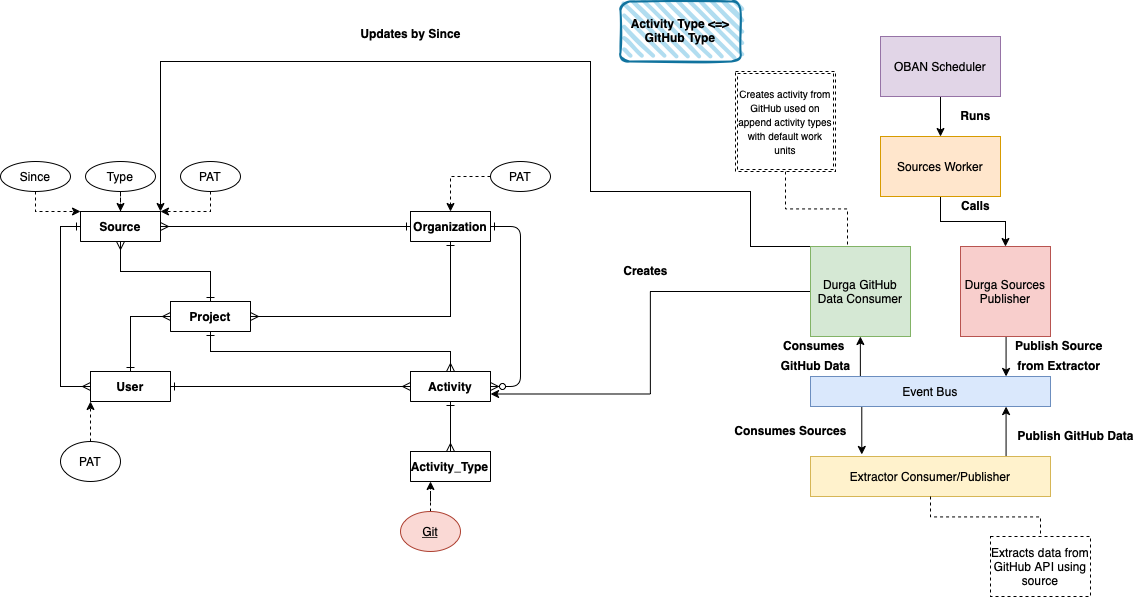
\includegraphics[scale=0.4]{Documentation/figures/diagram.png}  % largura percentual
	\caption{Entity-Relation and Workflow Diagram for Durga}
	\label{durga}
\end{figure}

\textbf{Key Components of the GitHub Data Extraction Life Cycle}

\begin{enumerate}
    \item \textit{Application Extractor}: The Application Extractor serves a vital function within the system, interacting directly with the GitHub API to fetch necessary data. It operates based on a publisher/consumer mechanism, subscribing to source events from the event bus and subsequently publishing GitHub data events. The interplay between subscription and publication establishes a fluid data pipeline from GitHub to Durga API app.
    \item  \textit{Durga GitHub Data Consumer}: This component acts as a subscriber to GitHub data events, transforming them into corresponding activity entries within the Durga API app. It identifies matches between the incoming GitHub data and valid activity types and associates them with the corresponding users through their GitHub handlers. One of its critical tasks is to update the \texttt{since} attribute on the sources, performed after successfully acknowledging the associated GitHub data for each source.
    \item \textit{Event Bus}: The Event Bus plays a critical role in the communication between the various components of the system. It is responsible for transmitting messages, which must adhere to a specific, enforced format to ensure the system accepts them. To facilitate the creation of new message types, a payload format must be defined. This task involves creating new \texttt{structs} for every accepted message type, ensuring data consistency, and enabling seamless communication across the system. 
    \item \textit{Sources Walker}: This worker already existed. It is responsible for checking the \texttt{since} attribute to ascertain the last update time for each source and then publishing a source event on the Event Bus. This regular crawling ensures that all sources are consistently monitored and any new activities are promptly identified and sent for further processing.
\end{enumerate}

The choice of an event bus architecture promotes fluid communication between applications that operate independently. These independent or 'decoupled' applications communicate through messages and remain agnostic to each other's internal workings. This design choice significantly simplifies scaling processes from a vertical and horizontal perspective. For example, if the workload related to data extraction experiences a surge - a likely scenario given that automated activity tracking constitutes a significant portion of Dharma Network's operations - multiple instances of the Extractor workers can be spawned effortlessly. These workers interconnected through the message bus, can efficiently distribute the workload among themselves and publish the results back to the same message bus.\newline

The Dharma Network team decided to adopt a decoupled architecture with a long-term vision in mind. By decoupling the applications, they could eliminate unnecessary dependencies and isolate potential faults, enhancing the system's overall resilience and flexibility. Furthermore, the modular approach fosters parallel development efforts, allowing teams to focus on a single component or service without being hindered by changes in others.\newline

In summary, the team's decision to choose a decoupled architecture was determined by the need for scalability, maintainability, resilience and development efficiency, which are vital for the ongoing success and growth of the Dharma Network.

\section{Development on Durga}

During the work on Durga, the main tasks that were assigned involved working within the Extractor and EventBus applications and creating a consumer within the Durga application. The work revolved around creating a complete lifecycle for data extraction from GitHub, beginning in Durga, proceeding through the Extractor, and then returning to Durga.

\subsection{Environment Variables}

The first official Dharma Network function to perform was to update the README.md. After the discovery of the crash of the program, it was necessary to update the README.md, so new developers could follow the rules. Information such as what Python version was compatible and the code lines that needed an update were added.\newline

Later, the implementation of environment variables was necessary. This feature had already been implemented on another project, as seen on section \ref{tentacat}, so the logic had already been taught.\newline

\textit{Environment variables} are variables set outside of the program and it's made up of a name/value pair. The whole point is to keep that information confidential.\newline

As for its implementation on Durga, they were set the following way: \newline

\begin{lstlisting}[language=erlang, caption={Environment Variables Configuration on .env.sample}]
# Remember to not leave any spaces between KEY and VALUE

 export JWT_SECRET=somekey

 export DEFAULT_PASS=anypassword

 # Username for the database
 export DATABASE_USERNAME=myusername

 # Password for the database
 export DATABASE_PASSWORD=mypassword

 # Name of the database
 export DATABASE_NAME=myapp_dev

 # Hostname for the database
 export DATABASE_HOST=host

 # Port for the database
 export DATABASE_PORT=port
\end{lstlisting}

\begin{lstlisting}[language=erlang, caption={Database configuration on dev.exs}]

 # Configure your database
 config :durga_api, DurgaApi.Repo,
   adapter: Ecto.Adapters.Postgres,
   username: System.get_env("DATABASE_USERNAME" || "database_name"),
   password: System.get_env("DATABASE_PASSWORD" || "database_password"),
   hostname: System.get_env("DATABASE_HOST" || "localhost"),
   database: System.get_env("DATABASE_NAME" || "developer_dev"),
   port: System.get_env("DATABASE_PORT" || "port_number"),
   stacktrace: true,
   show_sensitive_data_on_connection_error: true,
   pool_size: 15
\end{lstlisting}

This way, a developer can insert their information and it won't be stored when committing something on GitHub.\newline

\subsection{Extractor and Event Bus}

Once that was secured, it was time to work on what would be the most important feature developed and a key component of the entire project: the Extractor.\newline

The \textit{Extractor} followed the same lines of the Tentacat project (on section \ref{tentacat}). The solution was to develop a system that would extract the information requested by the user.\newline

This section already had some developed code, so the first interaction was not in terms of development, but of debugging. While debugging, it was clear to see that a significant portion of the provided code did not retrieve the expected information- or any information at all. Once the errors were specified, it was time to alter the existing code.\newline

Since the Extractor also had important information that was being stored on the code, environment variables were added. The Extractor needs information such as: \newline

\begin{lstlisting}[language=erlang, caption={Environment Variables Setup on extractor\_github.ex}]
token = System.get_env("GITHUB_TOKEN")
id = System.get_env("ID")
source_type = System.get_env("SOURCE_TYPE")
owner = System.get_env("GITHUB_OWNER")
user = System.get_env("GITHUB_USER")
repo = System.get_env("GITHUB_REPO")
since = System.get_env("SINCE_DATE")

\end{lstlisting}

As for the extraction of the GitHub information, it was made the following way:\newline

\begin{lstlisting}[language=erlang, caption={Commits extraction of extractor\_github.ex}]
@doc """
Shows every commit since given date, by all users
"""
def commits(token, id, org, repo, since) do
  client = Tentacat.Client.new(%{access_token: token})

  {_, commits, _} = Tentacat.Commits.filter(client, org, repo, %{
    since: since,
    per_page: 100
  })

  commits =
    commits
    |> Enum.filter(fn %{"parents" => parents} ->
      Enum.count_until(parents, 2) < 2
    end)
    |> Enum.map(&extract_commit/1)

  %{
    id: id,
    data: commits,
    source_type: :commits
  }
end
\end{lstlisting}

A client object is created using the \texttt{Tentacat} library (see \ref{tentacat}). The client is initialized with an access token.

It calls the \texttt{Tentacat.Commits.filter} function to retrieve a list of commits from a specified organization (\texttt{org}) and repository (\texttt{repo}). The \texttt{since} parameter specifies the starting date for the commits to retrieve, as the \texttt{per\_page} parameter limits the number of commits to be fetched to 100. If the filter wasn't selected, the default value would be 30. 

The result of this function call is a tuple containing three values, but the second value (commits) is of interest.

The \texttt{commits} list is then filtered using the texttt{Enum.filter function}. It checks each commit's "parents" field and keeps only those commits that have less than 2 parents. In other words, it \textit{filters out merge commits and keeps only the regular commits}.

The filtered commits are then transformed using the \texttt{Enum.map} function and a custom function \texttt{extract\_commit/1} is applied to each commit. The result is a new list of extracted commit data.

Finally, a map is constructed with the id, the filtered and extracted commits, and a \texttt{source\_type} field set to \texttt{:commits}. The map represents the result of the function.\newline


\begin{lstlisting}[language=erlang, caption={Pull requests extraction of extractor\_github.ex}]
@doc """
Shows every pull request since given date by a user (if specified) or all users (if null)
"""
def pull_requests(token, id, org, repo, since, user \\ nil) do
  client = Tentacat.Client.new(%{access_token: token})
  filters = %{state: "all", sort: "created", direction: "desc", creator: user, since: since}

  {_, pulls, _} = Tentacat.Issues.filter(client, org, repo, filters)

  pulls =
    Enum.filter(pulls, fn %{"user" => %{"login" => username}} ->
      is_nil(user) or username == user
    end)
    |> Enum.map(&extract_pull_request/1)

  %{
    id: id,
    data: pulls,
    source_type: :pull_requests
  }
end
\end{lstlisting}

 It creates a client using the \texttt{Tentacat.Client.new} function, passing the GitHub access token. Then, it defines the filters map containing the desired filter criteria, such as the state (can be open, closed or all), sort order (can be created, updated or comments), direction (can be ascending or descending), creator (the user that created the issue), and since date (timestamp in \texttt{ISO 8601} format: \textit{YYYY-MM-DDTHH:MM:SSZ}).\newline

 The \texttt{Tentacat.Issues.filter} function (see information on \ref{issue} to understand why we use \texttt{Issue} instead of \texttt{Pulls}) is invoked to retrieve the pull requests from the specified GitHub organization (\texttt{org}) and repository (\texttt{repo}) using the given filters. The result is stored in the pulls variable.\newline

The \texttt{Enum.filter} function is used to filter the pull requests based on the user parameter. If user is not \texttt{nil}, it only keeps the pull requests where the username matches the specified user. Otherwise, it keeps all pull requests. The filtered pull requests are then passed to the \texttt{Enum.map} function, which applies the \texttt{extract\_pull\_request/1} function to each pull request in order to extract the desired data.\newline

Finally, the function returns a map containing the id, data, and \texttt{source\_type} keys. The id is set to the provided id parameter, the data field holds the filtered and extracted pull requests stored in the pulls variable, and the \texttt{source\_type} is set to \texttt{:pull\_requests} to indicate the type of data retrieved.\newline

\begin{lstlisting}[language=erlang, caption={Reviews extraction of extractor\_github.ex}]
@doc """
Shows every review since given date and by given user (if specified) or all users (if null)
"""
def reviews(token, id, org, repo, since, user \\ nil) do
  client = Tentacat.Client.new(%{access_token: token})

  filters = %{sort: "created", direction: "desc", since: since}
  {_, comments, _} = Tentacat.Pulls.Comments.filter_all(client, org, repo, filters)

  reviews =
    Enum.filter(comments, fn %{"user" => %{"login" => username}} ->
      is_nil(user) or username == user
    end)
    |> Enum.map(&extract_review/1)

  %{
    id: id,
    data: reviews,
    source_type: :reviews
  }
end
\end{lstlisting}

It initializes the client using the \texttt{Tentacat.Client.new} function with the provided GitHub access token. The filters map is defined, specifying the sort order, direction, and since date for the comments.\newline

The \texttt{Tentacat.Pulls.Comments.filter\_all} function\footnote{This function was used because a review is considered if a pull request has two or more comments; if it only has one, it is considered a comment, so that information doesn't need to be retrieved.}\label{review} is called to retrieve all comments from the pull requests in the given GitHub organization (\texttt{org}) and repository (\texttt{repo}) based on the provided filters. The result is stored in the comments variable.\newline

The \texttt{Enum.filter} function is used to filter the comments based on the user parameter. If user is not \texttt{nil}, it only keeps the comments where the username matches the specified user. Otherwise, it keeps all comments. The filtered comments are then passed to the \texttt{Enum.map} function, which applies the \texttt{extract\_review/1} function to each comment in order to extract the desired data.\newline

Finally, the function returns a map containing the id, data, and \texttt{source\_type} keys. The id is set to the provided id parameter, the data field holds the filtered and extracted reviews stored in the reviews variable, and the \texttt{source\_type} is set to \texttt{:reviews} to indicate the type of data retrieved.\newline

\begin{lstlisting}[language=erlang, caption={Definition of private extraction functions of extractor\_github.ex}]
defp extract_commit(%{} = val) do
  val
end

defp extract_pull_request(%{} = val) do
  val
end

defp extract_review(%{} = val) do
  val
end
\end{lstlisting}

These extraction functions take a map as input and binds it to the variable val. The pattern \texttt{\%{} = val} matches any map. In this case, the functions don't perform any additional logic or transformation and simply return the input map val. They are used as helper functions.\newline

The EventBus was also implemented the following mode:\newline

\begin{lstlisting}[language=erlang, caption={Registry and Topics on event\_bus.ex}]
  @registry EventBus.Registry
  @topics [:source, :data]
\end{lstlisting}

\texttt{@registry} is a module attribute that holds the name of the registry used for event subscriptions. \texttt{@topics} is a module attribute that defines the list of supported topics.\newline

\begin{lstlisting}[language=erlang, caption={GenServer on event\_bus.ex}]
def start_link(_opts) do
  GenServer.start_link(__MODULE__, %{}, [{:name, __MODULE__}])
end
\end{lstlisting}

The \texttt{start\_link} function is the entry point for starting the \texttt{GenServer} process. It initializes the server state with an empty map \%{} and registers it with the name EventBus (the name of the module).\newline

\begin{lstlisting}[language=erlang, caption={Initialize state on event\_bus.ex}]
def init(state) do
  {:ok, state}
end
\end{lstlisting}

The \texttt{init} callback is called when the process is started and initializes the server state. In this code, it simply returns \texttt{\{:ok, state\}}.\newline

\begin{lstlisting}[language=erlang, caption={Subscribe to event topic on event\_bus.ex}, label={lst:unsub}]
def subscribe(key) do
  if Enum.member?(@topics, key) do
    {:ok, _} = Registry.register(EventBus.Registry, key, [])
    :ok
    case Registry.lookup(@registry, key) do
      [{pid, _}] ->
        {:ok, pid}
      [] ->
        {:ok, pid} = GenServer.start_link(__MODULE__, [], name: key)
        Registry.register(@registry, key, pid)
        {:ok, pid}
    end
  else
    :error
  end
end
\end{lstlisting}

The \texttt{subscribe} function is used to subscribe to a specific event topic. It takes a key parameter, which represents the topic to subscribe to. If the key is a member of the \texttt{@topics} list, it registers the topic in the \texttt{EventBus.Registry} and starts a new \texttt{GenServer} process for that topic if it doesn't already exist. It returns \texttt{:ok} if the subscription is successful, or \texttt{:error} if the key is not a supported topic.\newline

\begin{lstlisting}[language=erlang, caption={Unsubscribe to event topic on event\_bus.ex}]
def unsubscribe(key) do
  if Enum.member?(@topics, key) do
    Registry.unregister(@registry, key)
  else
    :error
  end
end
\end{lstlisting}

The \texttt{unsubscribe} function is used to unsubscribe from a specific event topic. It works the same way as the unsubscribe \ref{lst:unsub} does.\newline

\begin{lstlisting}[language=erlang, caption={Publish message on event\_bus.ex}]
def publish(:source, %EventBus.Messages.Source{} = payload) do
  publish_message(:source, payload)
end
def publish(:data, %EventBus.Messages.Data{} = payload) do
  publish_message(:data, payload)
end
\end{lstlisting}

The \texttt{publish} functions are used to publish messages to the event bus. They take a topic (\texttt{:source} or \texttt{:data}) and a payload as parameters. They call the private function \texttt{publish\_message} to handle the publishing of the message.\newline

\begin{lstlisting}[language=erlang, caption={Publish message's subscribers on event\_bus.ex}]
defp publish_message(key, payload) do
  Registry.dispatch(@registry, key, fn entries ->
    for {pid, _} <- entries, do: send(pid, {:publish, key, payload})
  end)
end
\end{lstlisting}

The \texttt{publish\_message} function retrieves the list of subscribers for the given key from the \texttt{EventBus.Registry} and sends the \texttt{\{:publish, key, payload\}} message to each subscriber process.\newline

\begin{lstlisting}[language=erlang, caption={Handle\_info on event\_bus.ex}]
def handle_info({:publish, key, payload}, state) do
  Logger.debug("Received message on topic #{inspect(key)} with payload: #{inspect(payload)}")
  case key do
    :source ->
      Logger.info("Received data from source: #{inspect(payload)}")
      {:noreply, state}
    :data ->
      Logger.info("Received data from data: #{inspect(payload)}")
      {:noreply, state}
    _ ->
      Logger.warn("Unsupported message: key=#{inspect(key)} payload=#{inspect(payload)}")
      {:noreply, state}
  end
end
\end{lstlisting}

The \texttt{handle\_info} callback is called when the server receives an asynchronous message. It handles messages of the form \texttt{\{:publish, key, payload\}}. It logs a debug message indicating the received message's topic and payload. Then, it matches the key to either \texttt{:source} or \texttt{:data} and logs an info message with the received payload. If the key doesn't match any known topic, it logs a warning message. Finally, it returns \texttt{\{:noreply, state\}} to indicate that no further action is required.\newline

Overall, the EventBus module provides a way to subscribe, unsubscribe and publish messages to different event topics, allowing communication between different processes in the application.\newline

When it comes to the connection with the Event Bus, the following was implemented:\newline

\begin{lstlisting}[language=erlang, caption={GenServer on extractor.ex}]
  def start_link(_opts) do
    GenServer.start_link(__MODULE__, %{}, [{:name, __MODULE__}])
  end
\end{lstlisting}

The \texttt{start\_link} function is the entry point for starting the \texttt{GenServer} process. It is responsible for initializing the server state and starting the process. In this case, it starts the Extractor process with an initial state of \%{} (an empty map) and registers it with the name Extractor (the name of the Module).\newline

\begin{lstlisting}[language=erlang, caption={Initialize state on extractor.ex}]
@impl true
def init(_state) do
  EventBus.subscribe(:source)
  {:ok, []}
end
\end{lstlisting}

The \texttt{init} callback is implemented as part of the \texttt{GenServer} behavior. It is called when the process is started and initializes the server state. In this code, it subscribes to the \texttt{:source} event on the EventBus and returns \texttt{\{:ok, []\}} as the initial state.\newline

\begin{lstlisting}[language=erlang, caption={Handle\_info for :source on extractor.ex}]
@impl true
def handle_info({:publish, :source, payload}, %{source: _source}) do
  GenServer.cast({:via, Registry, EventBus.Registry}, {:publish, :source, payload})

  {:noreply, state}
end
\end{lstlisting}

The \texttt{handle\_info} callback is called when the process receives an asynchronous message that is not handled by other specific message handlers. It handles the \texttt{\{:publish, :source, payload\}} message when the server state contains a key \texttt{:source}. It uses \texttt{GenServer.cast} to send a \texttt{\{:publish, :source, payload\}} message to the registered process via the Registry and EventBus.Registry. The return value \texttt{\{:noreply, state\}}indicates that no reply is sent to the sender of the message.\newline

\begin{lstlisting}[language=erlang, caption={Handle\_info for :data on extractor.ex}]
@impl true
def handle_info({:publish, :data, payload}, %{data: _data}) do
  GenServer.cast({:via, Registry, EventBus.Registry}, {:publish, :data, payload})

  {:noreply, state}
end
\end{lstlisting}

Similar to the previous \texttt{handle\_info} callback, this function handles the \texttt{\{:publish, :data, payload\}} message when the server state contains a key \texttt{:data}. It casts a \texttt{\{:publish, :data, payload\}} message to the registered process via the Registry and EventBus.Registry and returns \texttt{\{:noreply, state\}}.\newline

\begin{lstlisting}[language=erlang, caption={Handle\_info for key on extractor.ex}]
@impl true
def handle_info({:publish, key, payload}, state) do
  Logger.warn("Unsupported message: key=#{inspect(key)} payload=#{inspect(payload)}")

  {:noreply, state}
end
\end{lstlisting}

This is a fallback \texttt{handle\_info} callback that handles any other \texttt{\{:publish, key, payload\}} messages that are not explicitly matched by previous handlers. It logs a warning message indicating that an unsupported message was received, including the key and payload. It returns \texttt{\{:noreply, state\}}.\newline

This code handles incoming messages by either forwarding them to the registered process or logging a warning for unsupported messages.\newline

Amongst the development of this project, extensive testing and debugging were conducted to ensure its quality and reliability.\newline

\subsection{Publisher and Consumer}

The next step that wasn't fully completed was the creation of a publisher/consumer.\newline

A \textit{publisher} is a participant or entity responsible for generating and sending data or messages to a decentralized network or protocol.
The publisher is typically the source or originator of the information and initiates the process of sharing it with others.
They may publish data or messages through various means, such as posting on a decentralized platform, submitting transactions to a blockchain network or broadcasting messages to a peer-to-peer network.
The publisher may have specific intentions or objectives for sharing the data, such as disseminating news, providing updates or contributing to a decentralized application.\newline

As for the \textit{consumer}, it  is a participant or entity that receives and consumes data or messages from a decentralized network or protocol.
The consumer is interested in accessing or utilizing the information published by the publishers.
They retrieve data or messages from the network, typically by subscribing or requesting specific types of data they are interested in.
The consumer may process, analyze or use the received information for various purposes, such as displaying content to users, performing calculations or triggering specific actions.\newline

In decentralized systems, the publisher and consumer roles can be fulfilled by different participants or even automated processes. For example, in a decentralized messaging protocol, individual users can act as both publishers and consumers, sending and receiving messages to and from the network. Similarly, in a decentralized data marketplace, data providers act as publishers, offering their data for sale, while data buyers act as consumers, purchasing and utilizing the data.\newline

The objectives of this publisher are:

\begin{itemize}
    \item The publisher writes to the EventBus
    \item The publisher has its own API that can be called by other modules in the application
    \item Other modules can successfully publish extraction requests to Extractor.Github via the new publisher
    \item Extractor.Github successfully receives and processes the extraction requests sent by the new publisher.
\end{itemize}


As seen on figure \ref{durga}, Durga has an \texttt{Activity Type}, which will be fetched from GitHub by the consumer as follows:

\begin{lstlisting}[language=erlang, caption={Create Activity Type on activity\_consumer.ex}]
   defp create_commit_activities(<activity>) do
     activity_type = ActivityTypes.get_activity_type_by!(%{name: "github", description: "<description>"})
     [...]
\end{lstlisting}

\begin{lstlisting}[language=erlang, caption={Get Activity Type on activity\_types.ex}]
def get_activity_type_by!(params), do: Repo.get_by(ActivityType, params)
\end{lstlisting}

This way, it knows that the source is Github, since Dharma Network is planning on having multiple sources, like GitLab and others.\newline

The decoupled and modular architecture of the system was invaluable in this process. It allowed us to focus on specific system components, reducing dependencies on other parts and enhancing productivity. This practical experience provided a clear understanding of the benefits of such an architecture, further affirming the validity of the above design choices.\newline




 



\chapter{Analysis of the results}\label{chap:chap5}

This chapter contains a discussion of the results of the platform evaluation, as well as the program that was firstly shown and the program that ended up being developed.\newline

\section{Testing}

Effective backend testing is crucial for ensuring the reliability, functionality and security of the Dharma Network project.\newline

During the development of this project, the approaches used for backend testing in the Dharma Network were manual testing and unit testing. By examining the benefits and limitations of each approach, we can assess their effectiveness in ensuring the quality of the backend components.\newline

\subsection{Manual Tests}
Manual testing involves the systematic execution of test cases by human testers to validate the behavior and functionality of the backend system. In the context of the Dharma Network, manual testing plays a significant role in uncovering potential issues, verifying system responses and evaluating the overall user experience.\newline
\begin{comment}
    Some of the \textbf{benefits of Manual Testing} are:

\begin{itemize}
    \item \textit{Flexibility:} Manual testing allows testers to adapt and explore different test scenarios based on their knowledge and intuition. It enables the identification of edge cases and unexpected behaviors that may not be covered by automated tests.
    \item \textit{User Perspective:} Manual testing provides testers with an opportunity to evaluate the system from the perspective of end-users. It helps in validating the user interface, user interactions, and the overall usability of the backend system.
    \item \textit{Comprehensive Validation:} Manual testing enables testers to perform a comprehensive assessment of various functional and non-functional aspects, such as data validation, error handling, security vulnerabilities, and performance under real-world conditions.
\end{itemize}

However, some limitations of Manual Testing are:

\begin{itemize}
    \item \textit{Time-Consuming:} Manual testing can be time-consuming, especially when the system has a large codebase or frequent updates. Each test case needs to be executed manually, which may limit the number of tests that can be performed within a given timeframe.
    \item \textit{Human Error:} Manual testing is susceptible to human error. Testers may overlook certain scenarios or make mistakes during test execution, potentially leading to undetected issues or false results.
    \item \textit{Limited Test Coverage:} Due to time constraints and the human factor, it may not be possible to cover all possible test scenarios manually. This can result in gaps in test coverage and leave certain parts of the backend system untested.
\end{itemize}
\end{comment}

\subsection{Unit Tests}
Unit testing involves the creation of automated tests for individual units or components of the backend system. In the context of the Dharma Network, unit tests focus on verifying the behavior and correctness of specific functions, methods or classes.\newline
\begin{comment}
    Benefits of Unit Tests:

\begin{itemize}
    \item \textit{Automation:} Unit tests can be automated, allowing for faster and more frequent execution compared to manual testing. This enables developers to catch regressions early and maintain the stability of the backend system.
    \item \textit{Targeted Testing:} Unit tests provide targeted testing at the granular level, allowing for the identification of specific issues within isolated components. This helps in isolating and debugging problems, leading to more efficient troubleshooting.
    \item \textit{Test Coverage:} Unit tests facilitate higher test coverage by systematically examining individual components. Developers can create multiple test cases to cover various scenarios, ensuring a thorough examination of the backend system.
\end{itemize}

Limitations of Unit Tests:

\begin{itemize}
    \item \textit{Limited Scope:} Unit tests focus on individual units or components, meaning that they may not capture the interactions and dependencies between different parts of the backend system. Integration testing is required to validate the interactions and collaborations between these units.
    \item \textit{Incomplete System Validation:} Unit tests alone cannot provide a complete validation of the entire backend system. While they ensure the correctness of individual units, they may not uncover issues that arise from the integration of these units.
\end{itemize}
\end{comment}

To ensure a robust backend, a combination of manual testing and unit tests is recommended. Manual testing can focus on user experience, while unit tests can ensure the correctness and stability of individual components. The synergy between manual testing and unit tests contribute to the overall quality and success of the Dharma Network project.\newline

Here's an example of some of the tests performed:

\textbf{Test 1:}
\begin{enumerate}
    \item Leave empty values on the environment variables to see if they used the default ones
\end{enumerate}

\textbf{Test 2:}
\begin{enumerate}
    \item Introduce the default variables
    \item Introduce the information to retrieve- \texttt{commits}
    \item Compare retrieved information with information displayed on GitHub
\end{enumerate}

\textbf{Test 3:}
\begin{enumerate}
    \item Introduce the default variables
    \item Introduce the information to retrieve- reviews
    \item Compare retrieved information with the reviews on GitHub, keeping in mind the definition of review seen on section \ref{review}
\end{enumerate}

\textbf{Test 4:}
\begin{enumerate}
    \item Introduce the default variables
    \item Introduce the information to retrieve
    \item That information will have some empty fields, such as \texttt{user}, so it retrieves the information related to the entire team on that \texttt{since} date
    \item Compare retrieved information with the information on GitHub
\end{enumerate}

\section{Analysis of the project}

To begin the analysis, it is essential to understand the project's objectives. These objectives serve as the guiding principles that shape the project's direction and determine its success.\newline

As far as the objectives for this project, they have changed throughout the time.

\subsection{Initial vs. Final Sprint Distribution}\label{sprint}

The Sprint Distribution was one of the first things discussed, presented as pioneer plan by the company, during the first meeting, on January 11th 2023. On this meeting, Bruna and Emanuel dialogued about the languages and frameworks necessary for the project, as well as needed hardware, such as the MacBook Pro utilized during its development.\newline

A few weeks later, when the institutional protocols were signed and the internship was ready to start,  the first planning and distribution was presented (see figure \ref{sup_sch}).\newline

A Google Docs file with the entire period  and activities of the internship distributed by weeks was presented (see figure \ref{sup_days}).\newline

 \begin{figure}[htbp]
	\centering
	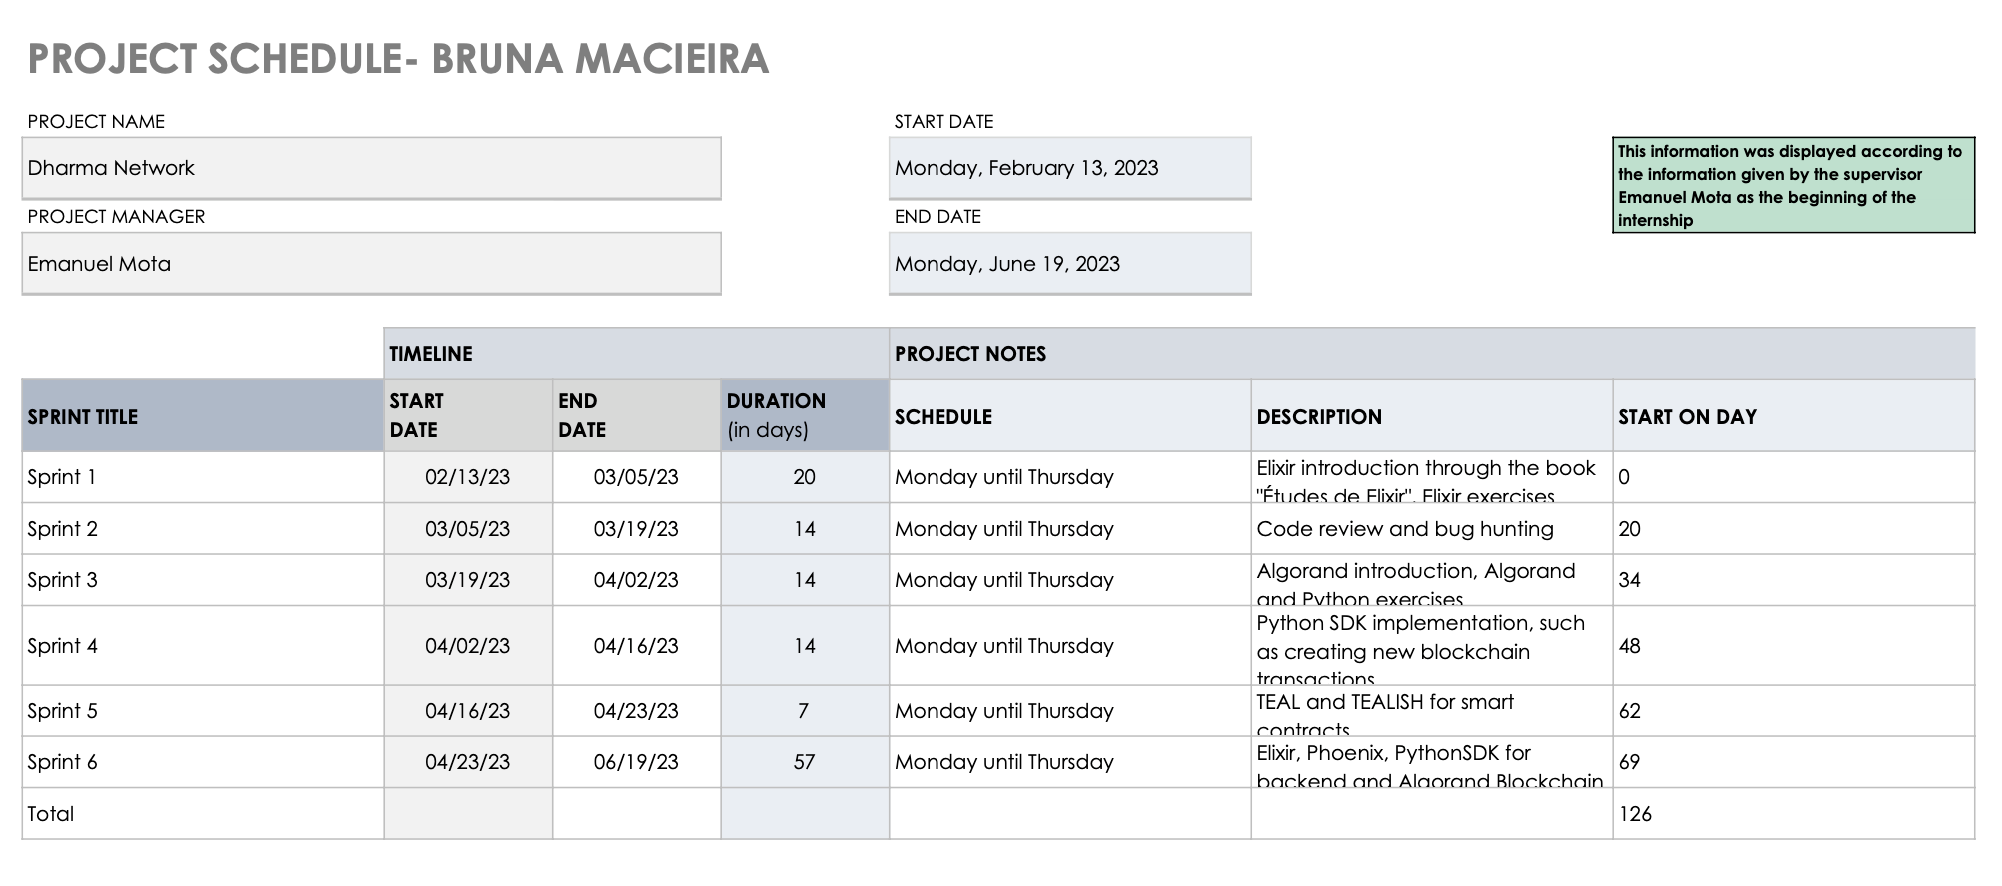
\includegraphics[scale=0.4]{Documentation/figures/sup_sch.png}  % largura percentual
	\caption{Intern's Initial Schedule}
	\label{sup_sch}
\end{figure}

 \begin{figure}[htbp]
	\centering
	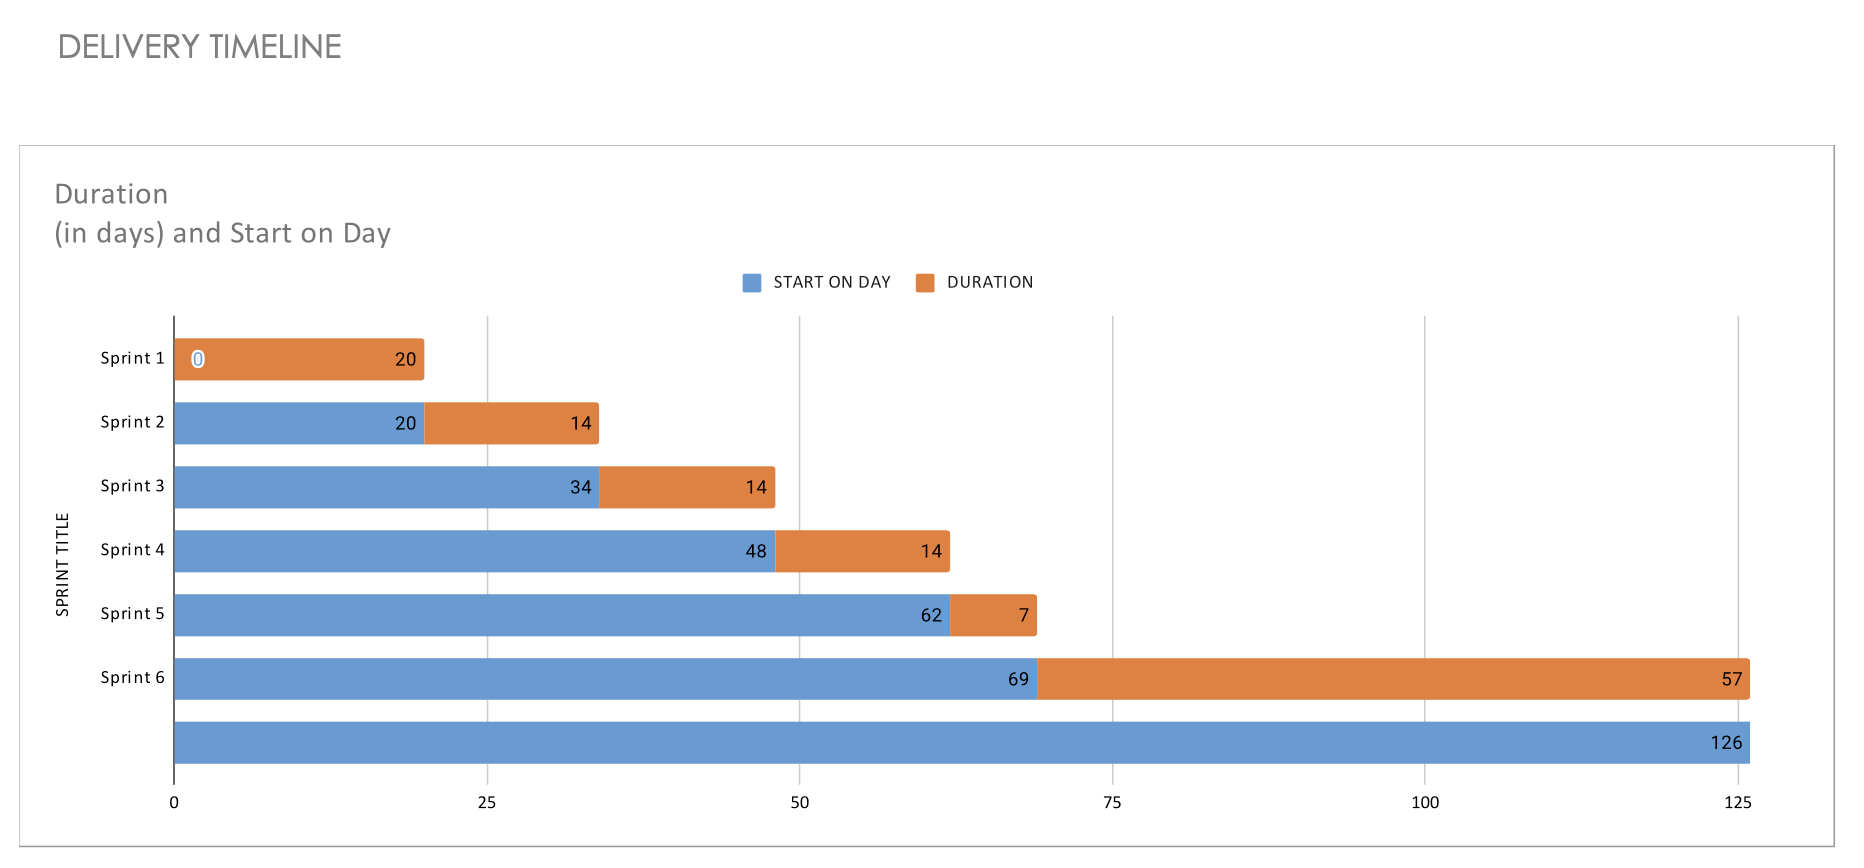
\includegraphics[scale=0.4]{Documentation/figures/sup_days.png}  % largura percentual
	\caption{Intern's Initial Sprint Distribution}
	\label{sup_days}
\end{figure}


However, due to the shortage of professionals working for Dharma Network and the need to advance the project, more experienced workers of the company developed the blockchain code, such as Smart Contracts and others.\newline

As a result, the project was developed according to the following guidelines on figures \ref{act_sch} and \ref{act_days}:\newline

 \begin{figure}[htbp]
	\centering
	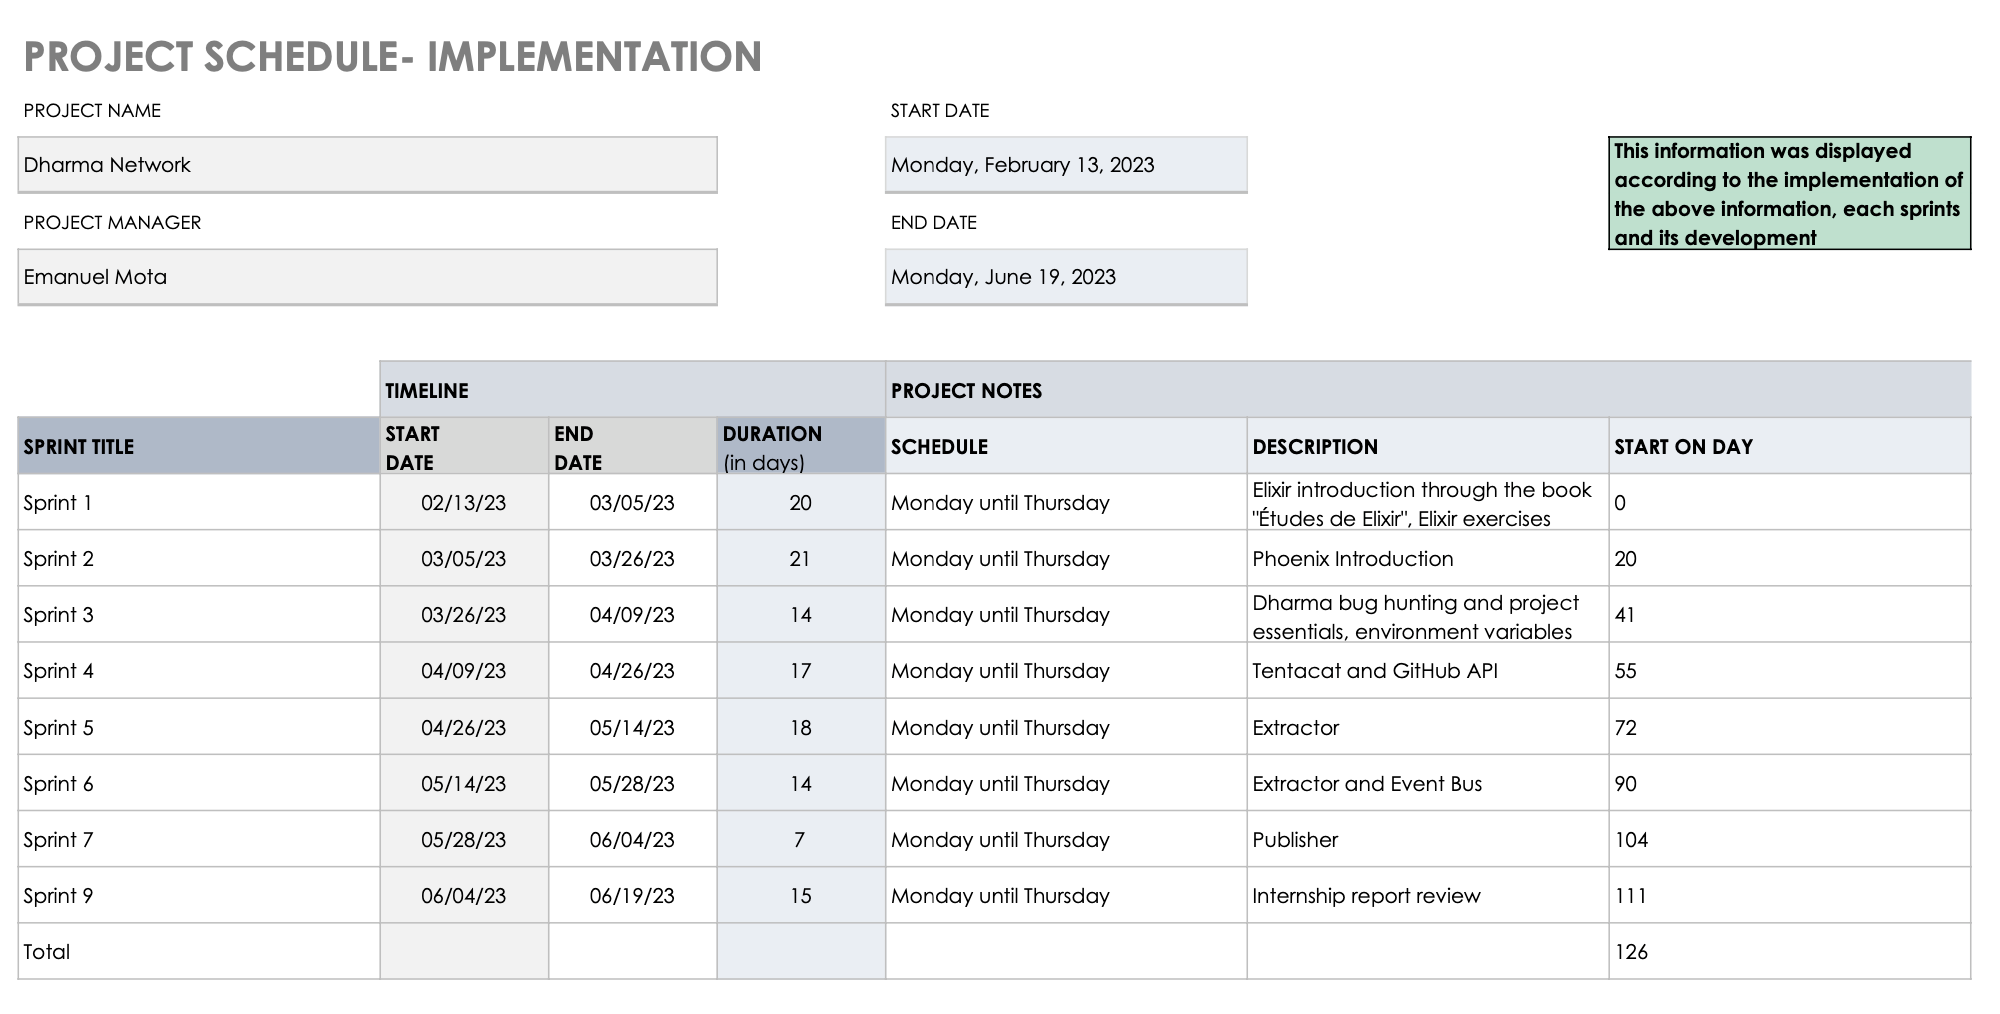
\includegraphics[scale=0.4]{Documentation/figures/act_sch.png}  % largura percentual
	\caption{Intern's Final Schedule}
	\label{act_sch}
\end{figure}

 \begin{figure}[htbp]
	\centering
	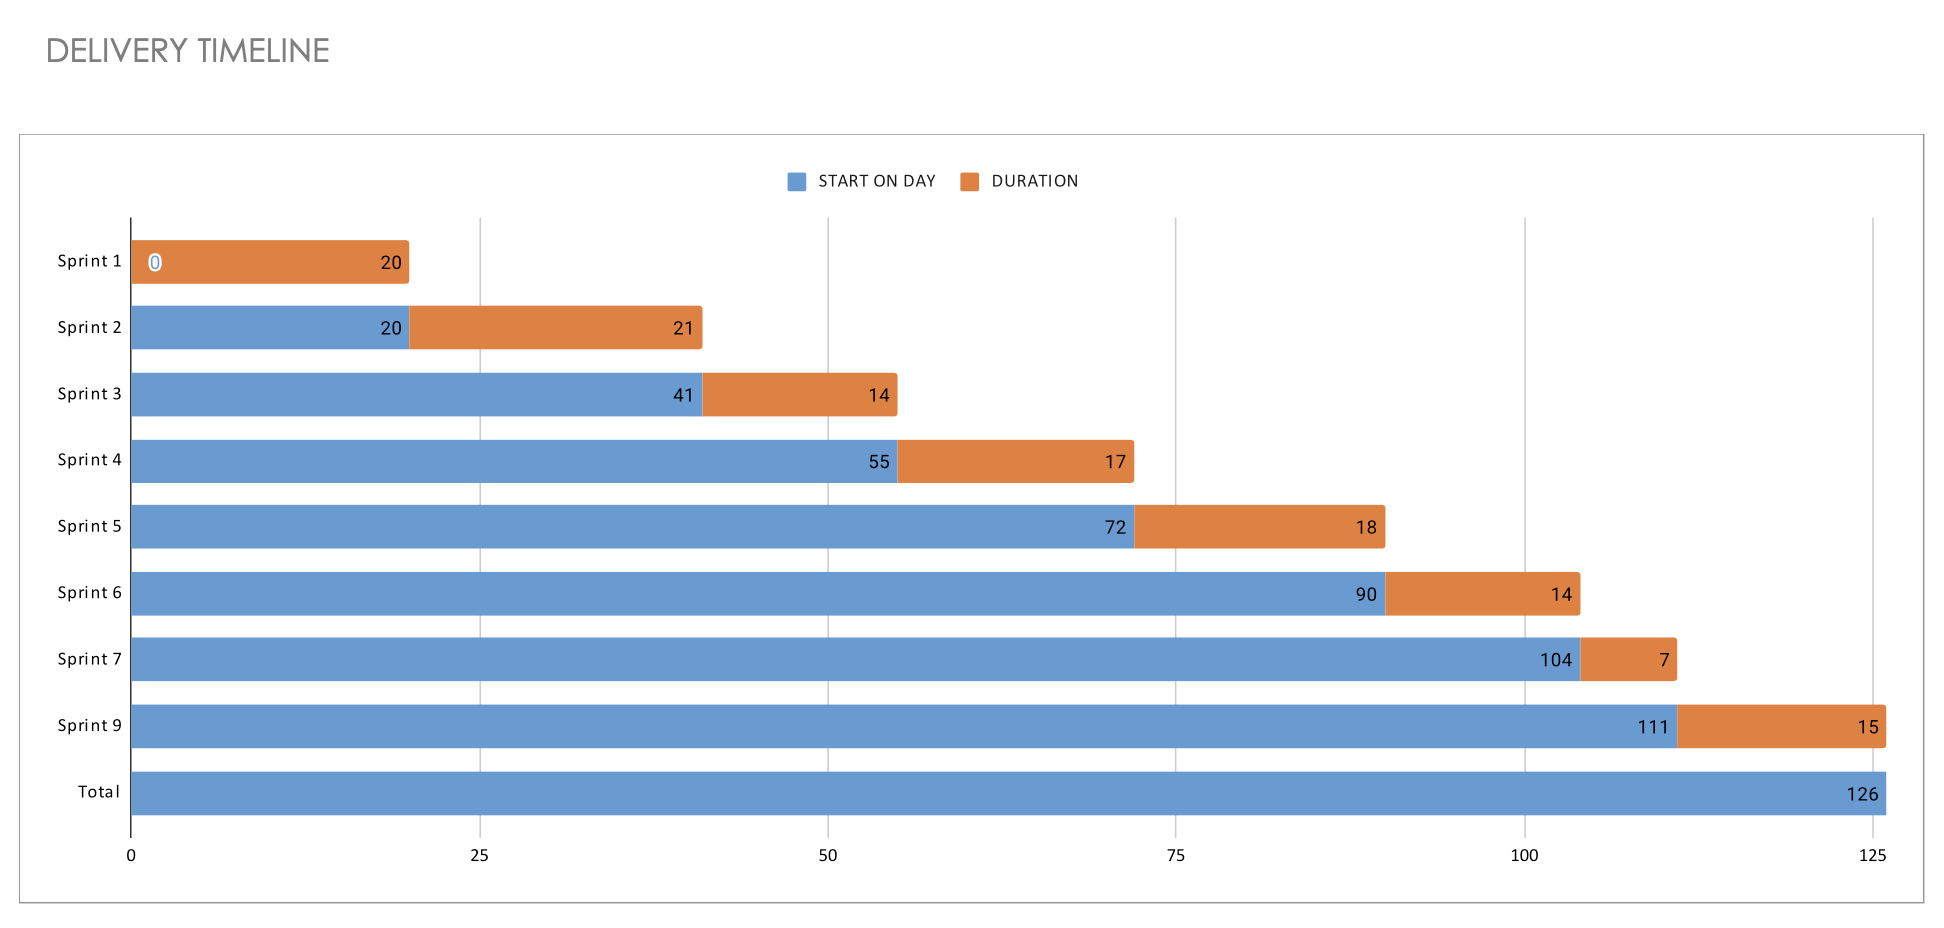
\includegraphics[scale=0.4]{Documentation/figures/act_days.png}  % largura percentual
	\caption{Intern's Final Sprint Distribution}
	\label{act_days}
\end{figure}

Figure \ref{sch} presents the hour counting of the internship and project distribution:


\begin{figure}[htbp]
	\centering
	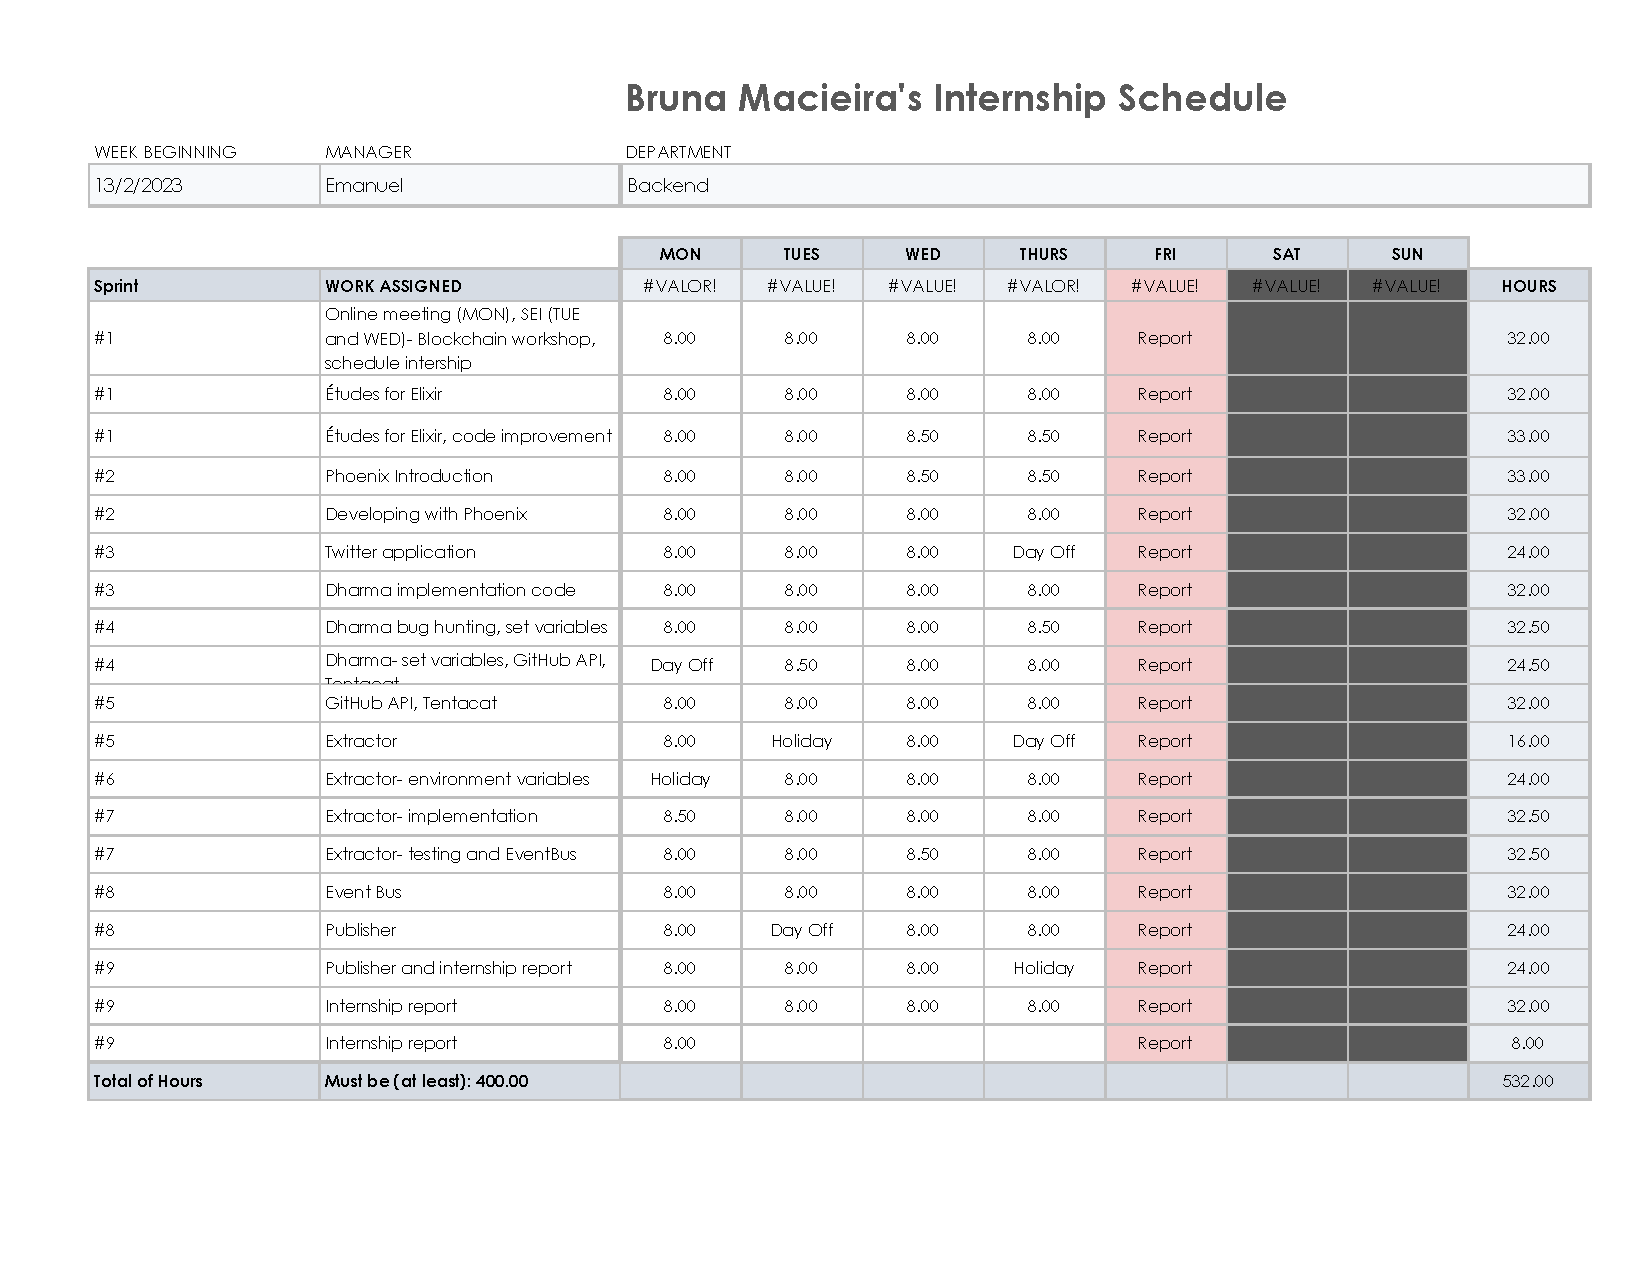
\includegraphics[scale=0.5]{Documentation/figures/Work_Hours - Work Schedule.pdf}  % largura percentual
	\caption{Intern's Internship Schedule and Hour Counting}
	\label{sch}
\end{figure}

\subsection{Final Analysis of the Project}

The blockchain components were built, but not by its original team. The backend components, however, were and continue to be developed by the original team.\newline

As far as the \textit{Proof of Real Work} of Dharma, it was implemented successfully, but it's not completed, since the publisher/consumer duo is not yet finished.\newline

The success of the Dharma Network project relies on continuous improvement and adaptation to evolving technological advancements, user demands and industry standards.
\chapter{Conclusions and future work} \label{chap:chap6}

In this final chapter, we will analyze the development of the project so far and draw conclusions based on the findings. We will also discuss future work and potential areas for improvement.

\section{Achievement of goals}

Working on this project has been an incredibly rewarding experience, as it has provided an opportunity to gain skills and knowledge that were previously thought to be attainable only through a master's degree. The project has allowed for personal growth and the development of essential technical skills.\newline

Throughout the project, there were moments of self-doubt and the feeling of being inadequate for the task at hand. However, overcoming challenges and successfully resolving issues, such as the bug encountered in section \ref{bug}, provided a sense of accomplishment and confidence in the project's progress.\newline

Additionally, the project has facilitated the improvement of collaboration skills, particularly in working with version control systems like GitHub. The ability to effectively manage and collaborate on code repositories is a valuable skill in the modern software development landscape.\newline

Given that the project deviated from the original sprint planning, it becomes challenging to definitively assess the achievement of the goals. However, considering the work undertaken, it is apparent that significant progress was made towards attaining the goals and the project served as an invaluable catalyst for personal and professional development.\newline

\section{Future work}

\\As Dharma Network progresses, future work will focus on several key areas. The establishment of a Dharma Network Foundation will provide legal support and transition towards a Decentralized Autonomous Organization (DAO). The Dharma DAO will enable token holders to participate in governance and decision-making processes. Furthermore, the expansion of liquidity pools, fee adjustments, and grants for projects aligned with the Dharma Network's vision will be explored in later phases.\\

Moving forward with Dharma Network, there are several areas that warrant further attention and future work. These include:

\begin{enumerate}
    \item \textit{Establishing a Dharma Network Foundation:} Creating a legal entity to support the Dharma Network will provide a solid foundation for governance and facilitate the transition towards a Decentralized Autonomous Organization (DAO). The DAO structure will enable token holders to participate in decision-making processes and shape the future direction of the project.
    \item \textit{Expanding Liquidity Pools and Fee Adjustments:} The project should explore strategies to increase liquidity pools within the Dharma Network. This can be achieved through partnerships, incentivizing liquidity providers, and adjusting transaction fees to maintain a healthy and sustainable ecosystem.
    \item \textit{Grants for Aligned Projects:} Offering grants and support to projects aligned with the Dharma Network's vision will foster innovation and growth within the ecosystem. This will encourage developers and entrepreneurs to build on the platform and contribute to its expansion.
\end{enumerate}

In conclusion, future work should focus on governance, liquidity expansion and fostering a vibrant ecosystem of projects within the Dharma Network.

\section{The Future of DeFi}

The future of decentralized finance holds immense potential for reshaping the global financial landscape and addressing income inequality. By providing accessible, transparent and inclusive financial services, DeFi has the power to empower individuals and communities that have been historically marginalized. However, several challenges and considerations must be addressed to ensure the long-term success and sustainability of the DeFi ecosystem.\newline

Technological barriers, regulatory frameworks and infrastructure limitations remain as hurdles that need to be overcome to achieve widespread adoption and inclusivity. Efforts must be made to bridge the digital divide and provide education and awareness about DeFi to underserved communities. Collaboration between governments, financial institutions and technology innovators is crucial to harness the full potential of decentralized finance in tackling global income inequality.\newline

The governance structures within DeFi projects need careful attention to ensure accountability, transparency and fairness. Clear mechanisms for decision-making and community involvement are vital to protect the interests of participants and maintain the integrity of the network. Additionally, addressing potential risks associated with the gamification of finance and promoting responsible market behavior will contribute to the long-term stability of the DeFi ecosystem \cite{oecd}.\newline

Despite these challenges, the transformative power of decentralized finance should not be underestimated. As we navigate the evolving DeFi landscape, it is essential to prioritize innovation, collaboration, and responsible development. By addressing these challenges and fostering an inclusive and sustainable DeFi ecosystem, we can ensure that the benefits of decentralized finance are shared by all, contributing to a more equitable and inclusive financial future.\newline


\begin{comment}
    However, challenges remain. Technological barriers, regulatory frameworks and infrastructure limitations, such as poor or no access to the Internet, must be addressed to ensure widespread adoption and inclusivity. Moreover, efforts must be made to bridge the digital divide and provide education and awareness about DeFi to underserved communities. Collaboration between governments, financial institutions and technology innovators is crucial to harness the full potential of decentralized finance in tackling global income inequality.

Decentralized finance and cryptocurrencies have the potential to reshape the global financial landscape and address the persistent issue of income inequality. By providing accessible, transparent, and inclusive financial services, DeFi can empower individuals and communities that have been historically marginalized. While challenges exist, the transformative power of decentralized finance should not be underestimated. As we navigate this evolving landscape, it is essential to prioritize innovation, collaboration, and responsible development to ensure that the benefits of DeFi are shared by all.
\end{comment}

Moreover, one of the significant challenges faced by the decentralized finance industry is the carbon emissions associated with the mining processes. As the environmental impact of blockchain networks becomes more apparent, addressing carbon footprints has become a pressing concern. In this regard, the next significant step for Dharma Network could be to explore ways of making the mining process of their token carbon-neutral.\newline

The significance of addressing carbon emissions in the blockchain space becomes evident when compared to the energy consumption of entire countries. For instance, Bitcoin consumes around 130 terawatt-hours (TWh) of energy annually, which is comparable to the energy consumption of countries like Sweden (131 TWh), Norway and Argentina (both around 125 TWh). It is nearly triple the energy consumption of Portugal, which is approximately 48 TWh per year \cite{ns}.\newline

Algorand's energy consumption is known to be relatively low compared to other blockchain networks. According to the CTO of Algorand Foundation, Algorand uses only 80 kW of energy and incorporates carbon offsetting measures into its operations, making it one of the most eco-friendly blockchain networks available \cite{daddy, tel}.\newline

What about the carbon footprint of Dharma Network? Although it's unknown, Dharma Network is built on top of the Algorand blockchain, so it's clear to say that Dharma Network can also be considered a low carbon footprint project. 


\section{Conclusion}

In conclusion, Dharma Network represents an innovative and disruptive solution in the realm of decentralized finance. By combining the power of the Algorand blockchain, robust backend services and a community-driven governance structure, Dharma Network strives to democratize access to financial services and foster a truly decentralized and inclusive ecosystem.\newline

Dharma Network has the potential to empower employees by embracing the ethos that "(...) graduate worker or master's degree holder, we are all workers" (José Teixeira, DST's CEO, in \textit{"É ou Não É"}, RTP). In this paradigm, the traditional barriers that differentiate individuals based on their educational backgrounds are diminished, as the focus shifts to valuing the contributions and skills of every worker. By providing equal opportunities for participation and leveraging the power of blockchain technology, Dharma Network enables individuals to harness their potential and compete on a level playing field. As José Teixeira, DST's CEO, aptly stated, "(...) the freer individuals are, the more competitive they tend to be", which also brings an advantage to the company, since "(...) we use resources because it brings a competitive advantage" (José Teixeira, DST's CEO, in \textit{"É ou Não É"}, RTP). With Dharma Network, employees can leverage their skills, tap into a decentralized financial ecosystem and capitalize on resources to gain a competitive advantage in the global marketplace. \newline

\begin{comment}
    There are certain issues that may occur with such projects:

\begin{enumerate}
    \item \textbf{Lack of Accountability:}\newline

    \textit{Problem:}
    
    The decentralized nature of DeFi projects can lead to a lack of accountability for those launching open protocols. Initial VC (Venture Capital\footnote{Venture Capital is a form of private equity and financing that investors provide to businesses they believe to have long-term growth}) funders and core developers often retain governance tokens, but the size of their holdings may not be transparent to users or regulators \cite{oecd}.

    \textit{Dharma Network's solution:}

    \item \textbf{Community Splits and Forks:}\newline

    \textit{Problem:}

     Contentious decisions within the community can result in network splits and forks. In proof-of-work systems, like Bitcoin and Ethereum, miners with majority control can influence transaction validation and the future direction of the chain. It may be unclear how protocol changes affecting existing contracts are decided by the community \cite{oecd}.

    \textit{Dharma Network's solution:}

    \item \textbf{Gamification of Finance:}\newline

    \textit{Problem:}

     The gamification of DeFi platforms can attract inexperienced investors, potentially leading to irrational trading and reliance on unsound financial advice. These issues relate to consumer protection and may impact market behavior and financial stability. Loss of confidence in DeFi could affect traditional financial systems \cite{oecd}.

    \textit{Dharma Network's solution:}
\end{enumerate}
\end{comment}







%%----------------------------------------
%% Final materials
%%----------------------------------------

%% Bibliography
%% Comment the next command if BibTeX file not used
%% bibliography is in ``myrefs.bib''
\PrintBib{myrefs}

%% comment next 2 commands if numbered appendices are not used
\appendix
\chapter{Group organisation dossier} \label{groupdossier}

\section{Internal Rules}

\subsection{Scope}
The purpose of this document is to provide a comprehensive overview of the internship experience by documenting and showcasing the activities, projects and achievements of the intern, Bruna Macieira. It aims to capture the collective efforts and individual contributions of the intern throughout the internship period. The dossier will serve as a valuable resource for the organization, supervisors and the intern herself.

\subsection{Meetings}

\begin{itemize}
\item Team meetings are scheduled to be held daily, unless otherwise notified in advance.

\item In case of more significant commitments, meetings can be rescheduled accordingly.

\item Extraordinary meetings may be scheduled as needed.

\item Notices will be issued solely for extraordinary meetings.

\item Concise meeting minutes are used to summarize the discussed topics.
\end{itemize}


\section{Calendar- Sprint Distribution and Daily Records}

The following figure (see \ref{fig:cal} and \ref{fig:cap}) is divided into sprints and each day has a record about what was made on that day. The records can be seen \href{https://docs.google.com/spreadsheets/d/1pNtDSX2snoRg8GJPjER8w_auBMuyReotaNJmS4W0FGc/edit#gid=649548965}{here}.

\begin{figure}[htbp]
	\centering
	
	\begin{minipage}[b]{0.55\textwidth}
		\centering
		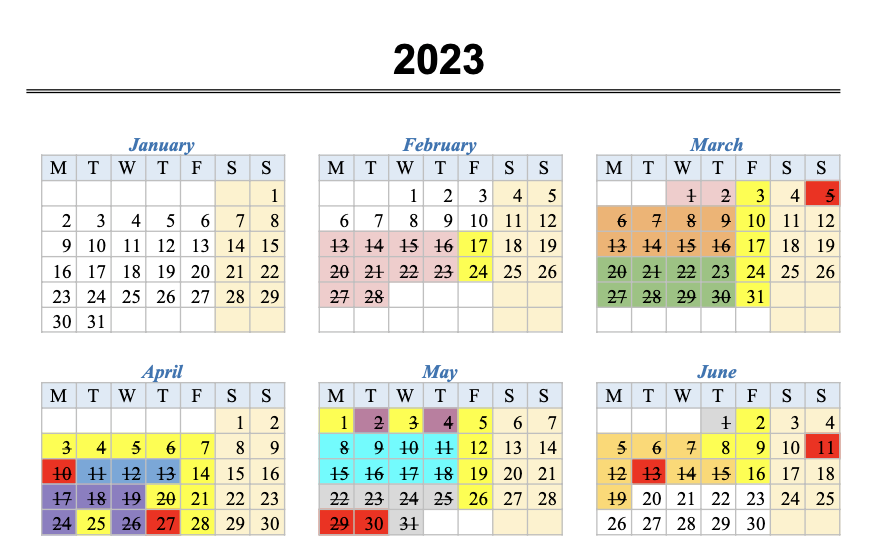
\includegraphics[width=\linewidth]{Documentation/figures/cal.png}
		\caption{Calendar with Sprint Distribution and Daily Records}
		\label{fig:cal}
	\end{minipage}
	\hfill
	\begin{minipage}[b]{0.40\textwidth}
		\centering
		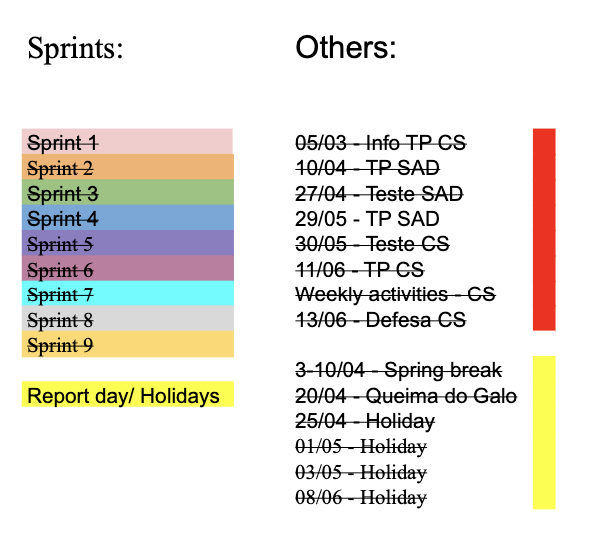
\includegraphics[width=\linewidth]{Documentation/figures/leg.png}
		\caption{Calendar's caption}
		\label{fig:cap}
	\end{minipage}

\end{figure}

\noindent \rule{\linewidth}{0.4pt}
\newline


%% Index
%% Uncomment next command if index is required
%% don't forget to run ``makeindex thesis'' command
%\PrintIndex


\end{document}
